%
% LaTeX template for prepartion of submissions to PLDI'15
%
% Requires temporary version of sigplanconf style file provided on
% PLDI'15 web site.
%
%% \documentclass[pldi]{sigplanconf-pldi15}
%old header
%\documentclass[preprint,10pt, numbers]{sigplanconf}

% new 2019 header
%\documentclass[sigplan,10pt,review,anonymous]{acmart}\settopmatter{printfolios=true,printccs=false,printacmref=false}

% removing "review" from new header
%\documentclass[sigplan,10pt,anonymous]{acmart}\settopmatter{printfolios=true,printccs=false,printacmref=false}

% The above is legacy from the old PLDI submissions
% Below I'm trying out the OOPSLA format

%% For double-blind review submission, w/o CCS and ACM Reference (max submission space)
\documentclass[acmsmall,anonymous]{acmart}\settopmatter{printfolios=true,printccs=false,printacmref=false}

%% Journal information
%% Supplied to authors by publisher for camera-ready submission;
%% use defaults for review submission.
\acmJournal{PACMPL}
\acmVolume{1}
\acmNumber{OOPSLA} % CONF = POPL or ICFP or OOPSLA
\acmArticle{1}
\acmYear{2019}
\acmMonth{1}
\acmDOI{} % \acmDOI{10.1145/nnnnnnn.nnnnnnn}
\startPage{1}

\setcopyright{none}
\bibliographystyle{ACM-Reference-Format}
\citestyle{acmauthoryear}   %% For author/year citations


%
% the following standard packages may be helpful, but are not required
%

\usepackage[utf8]{inputenc}
\usepackage[T1]{fontenc}
%\usepackage[tbtags]{amsmath} %\usepackage{amsmath}
\usepackage{mathtools}
\usepackage{mathpartir}
\usepackage{listings}          % format code
\usepackage{stmaryrd}
\usepackage{relsize}
\usepackage{setspace}
\usepackage[small,compact]{titlesec}

\usepackage{amssymb}
\usepackage{savesym}
\savesymbol{bigtimes}
\usepackage{mathabx}
\restoresymbol{ABX}{bigtimes}
\usepackage{wasysym}
%% \usepackage{SIunits}            % typset units correctly
\usepackage{courier}            % standard fixed width font
\usepackage[scaled]{helvet} % see www.ctan.org/get/macros/latex/required/psnfss/psnfss2e.pdf
\usepackage{url}                  % format URLs
\usepackage{enumitem}      % adjust spacing in enums
% known bug: http://tex.stackexchange.com/questions/1522/pdfendlink-ended-up-in-different-nesting-level-than-pdfstartlink
%\usepackage{tikz}
\long\def\beginpgfgraphicnamed#1#2\endpgfgraphicnamed{\includegraphics{#1}}
%% \usetikzlibrary{arrows.meta, positioning, decorations.pathmorphing, fit}
%% \pgfrealjobname{autoquack}
\usepackage{fancybox}
\usepackage{multicol}
\usepackage{semantic}
\newcommand{\triple}[3]{\{#1\}\,#2\,\{#3\}}
\newcommand{\doi}[1]{doi:~\href{http://dx.doi.org/#1}{\Hurl{#1}}}   % print a hyperlinked DOI
\usepackage{mathtools}
\usepackage{tablefootnote}
%\usepackage{placeins}

\newcommand\hide[1]{}

\newcommand{\scon}{\mathbin{\varstar}}
\newcommand{\ocon}{%
  \mathbin{\mbox{$\mathrlap{\cup}\hspace*{.15em}
      \raisebox{.01em}[0ex][0ex]{$\scon$}$\hspace*{.07em}}}}
\newcommand{\wand}{%
 \mathrel{\mbox{$\hspace*{-0.03em}\mathord{-}\hspace*{-0.66em}
     \mathord{-}\hspace*{-0.36em}\mathord{\scon}$\hspace*{-0.005em}}}}
\newcommand{\septraction}{%
  \mathrel{\mbox{$\hspace*{-0.03em}\mathord{-}\hspace*{-0.66em}
  \mathord{-}\hspace*{-0.155em}\mathord{\ocircle\hspace*{-.66em}\scon}$\hspace*{0.05em}}}}
\newcommand{\magicwand}{\wand}
\newcommand{\defeq}{\mathbin{\stackrel{\Delta}{=}}}

\newcommand{\bigocon}{
  \raisebox{-0.3ex}{\resizebox{0.75em}{!}{$\scon$}} \hspace{-4.3ex} \bigcup}
\newcommand{\medocon}{
  \raisebox{-0.3ex}{\resizebox{0.63em}{!}{$\scon$}} \hspace{-2.05ex} \bigcup}

%\input mathlig
  \mathlig{--*}{\mathrel{\magicwand}}
  \mathlig{--o}{\mathrel{\septraction}}
  \mathlig{|->}{\mathrel{\mapsto}} % tight points-to
  \mathlig{<=>}{\mathrel{\Leftrightarrow}} % equivalence of expressions
  \mathlig{==>}{\mathrel{\Rightarrow}} % meta implication
  \mathlig{-|-}{\mathrel{\mathrlap{\dashv} \hspace{5pt} \vdash}} % entails

\hide{
  \mathlig{||-}{\mathbin{\Vdash}}
  \mathlig{<==>}{\mathrel{\Longleftrightarrow}} % equivalence
  \mathlig{--->}{\mathrel{\longrightarrow}} % transitions
  % 3 chars
  %\mathlig{::=}{\mathrel{\Coloneqq}}
  \mathlig{-->}{\mathrel{\rightarrow}} % set function space
  \mathlig{<->}{\mathrel{\leftrightarrow}}
  \mathlig{-|}{\dashv}
  \mathlig{--`}{\mathrel{\rightharpoonup}} % partial function
  \mathlig{===}{\mathrel{\equiv}} % syntactic equality
  \mathlig{=/=}{\mathrel{\not\equiv}} % not syntactic equality
  \mathlig{|/-}{\nvdash} % not entailment
  \mathlig{|/=}{\nvDash} % not forces
  \mathlig{|||}{\mathrel{|}} % grammar
  \mathlig{||=}{\VDash}
  \mathlig{||-}{\Vdash}
  % 2 chars
  \mathlig{==}{\mathrel{\stackrel{\smash{\scriptscriptstyle\mathrm{def}}}{=}}}
% \mathlig{==}{\mathrel{\triangleq}}
}
  \mathlig{/|}{\mathbin{\wedge}} % additive conjunction
  \mathlig{|/}{\mathbin{\vee}} % additive disjunction
  \mathlig{|-}{\mathrel{\vdash}} % entails
  \mathlig{|=}{\vDash} % models
\hide{
  \mathlig{/=}{\mathrel{\neq}} % non-equality expression
  \mathlig{<=}{\mathord{\leq}} % less than or equal expression
  \mathlig{=>}{\mathrel{\Rightarrow}} % implication
  \mathlig{|>}{\vartriangleright}
  \mathlig{<|}{\vartriangleleft}
  \mathlig{[|}{\llbracket} % open double bracket
  \mathlig{|]}{\rrbracket} % close double bracket
  \mathlig{->}{\mathord{\rightarrow}} % field dereference
  \mathlig{<-}{\mathord{\leftarrow}} % assignement
}

  \mathlig{**}{\mathbin{\ocon}}
  \mathlig{*}{\mathbin{\scon}}

%\usepackage{common}
%\usepackage{seplog}


% inline code
\makeatletter
\newlength{\@mli}
\newcommand{\mli}[1]{%
  \settowidth{\@mli}{\lstinline/#1/}
  \hspace{-.5ex}\begin{minipage}[t]{\@mli}\lstinline/#1/\end{minipage}}
\makeatother
\newcommand{\li}[1]{\ifmmode\mbox{\mli{#1}}\else\mbox{\lstinline/#1/}\fi}

\newcommand{\tx}[1]{\text{#1}}
\newcommand{\p}[1]{\ensuremath{\mathsf{#1}}} % predicate font
\newcommand{\m}[1]{\ensuremath{\mathit{#1}}} % math font
\newcommand{\ramify}{\mbox{\lightning}}
\newcommand{\infrulestyle}[1]{\textsc{#1}}
\newcommand{\infrule}[4]{\inferrule*[lab=\infrulestyle{#1},right=$\mathrlap{#4}$]{#2}{#3}}
\newcommand{\RuleS}[4]{\infrulestyle{#1}\frac{#2}{#3} \textit{#4}}
\newcommand{\Rule}[3]{\[\RuleS{#1}{\begin{array}{c} #2 \end{array}}{#3}{}\]}
\newcommand{\MV}{\ensuremath{\mathsf{ModVar}}}
\newcommand{\FV}{\ensuremath{\mathsf{FreeVar}}}
\newcommand{\pguards}[1]{\llbracket #1 \rrbracket}


\lstset{%
  language=C,
  morecomment=[n][{\color{red!80!black}}]{/*}{*/},
  morecomment=[l][{\color{red!80!black}}]{//},
  sensitive=true,
  mathescape=true,
  showlines=true,
  basicstyle=\normalfont\smaller\tt,
  keywordstyle=\color{blue},
  numbers=left,
  numberstyle=\tiny,
  numbersep=5pt,
  boxpos=t,
}


%\lstset{language=C,basicstyle=\small,mathescape=true,columns=fullflexible}


\begin{document}
\special{papersize=8.5in,11in}
\setlength{\pdfpageheight}{\paperheight}
\setlength{\pdfpagewidth}{\paperwidth}
%\conferenceinfo{CONF 'yy}{Month d--d, 20yy, City, ST, Country}
%\copyrightyear{20yy}
%\copyrightdata{978-1-nnnn-nnnn-n/yy/mm}
%\copyrightdoi{nnnnnnn.nnnnnnn}

%
% any author declaration will be ignored  when using 'plid' option (for double blind review)
%

%\title{The Ramifications of Mechanizing Verification}
\title{Certifying Graph-Manipulating C Programs \\ via Localizations within Data Structures}
%\authorinfo{Shengyi Wang$^{*}$ \qquad Qinxiang Cao$^{+}$ \qquad Asankhaya Sharma$^{*}$ \qquad Aquinas Hobor$^{\dagger,*}$}
%{}
%{School of Computing$^{*}$ and Yale-NUS College$^{\dagger}$, National University of Singapore; Princeton University$^{+}$}
%\authorinfo{} {} {}

\begin{abstract}
We develop powerful and general techniques to mechanically verify realistic programs that
manipulate heap-represented graphs and related data structures with intrinsic sharing.
We construct a modular and general setup for reasoning about abstract mathematical graphs
and use separation logic to define how such abstract graphs are represented concretely in
the heap.  {\color{magenta}We upgrade Hobor and Villard's theory of ramification 
to support existential
quantifiers in postconditions and to smooth the treatment of modified program variables
so that we can use it to verify real graph-manipulating C code.}
{\color{blue}I wonder if this should be shortened for the abstract... 
``We make {\color{magenta}two} improvements to Hobor and 
Villard's theory of ramification 
and use our improved version to verify real graph-manipulating C code.''}  
We demonstrate the generality
and power of our techniques by integrating them into the Verified Software Toolchain and
certifying the correctness of seven graph-manipulating programs written in 
CompCert C, including
a 400-line generational garbage collector for the CertiCoq project.  
While doing so, we identify
two places where the C semantics is too weak to define generational 
garbage collectors of the
sort used in the OCaml runtime.  Our proofs are entirely machine-checked.
%We connect our development to two large verification tools, and HIP/SLEEK, and use these tools to mechanically verify several canonical graph algorithms. %
\end{abstract}

\keywords{keyword1, keyword2, keyword3}  %% \keywords are mandatory in final camera-ready submission

\maketitle

\section{Introduction}
\label{sec:intro}

Dijkstra's eponymous shortest-path algorithm~\cite{Dijk} finds
the cost-minimal paths from a distinguished \emph{source} vertex
source to all reachable vertices in a finite directed graph.

The algorithm is classic and ubiquitous, appearing widely in textbooks
and in real routing protocols. Further, the algorithm has been in
use for over $60$ years, suggesting, for all practical purposes,
that its safety and correctness have been verified by decades of application.

Recent efforts [cite Mizar, cite ACL2, cite Coq] have implemented the algorithm
in proof assistants and formally proved claims about its behavior.
However, because they operate entirely within idealized formal checkers,
these works inadvertently gloss over certain classes of issues
that routinely crop up in real-world settings.

In this paper we verify a~C~implementation of Dijkstra's
one-to-all shortest path algorithm. We implement
textbook~C~code [cite CLRS], import it into Coq [cite VST],
and state and prove a correctness claim in Coq [cite VST, cite RamifyCoq].
We expose a subtle overflow issue in the code, and address the issue
via a nontrivial refinement in the precondition of the algorithm.

The paper is organized as follows:
\vspace{-1em}
\begin{itemize}
    \item[\S\ref{sec:overview}] We briefly present and explain
    our~C~implementation of Dijkstra's algorithm.
    \item[\S\ref{sec:verification}] We present our specification
    and our most important loop invariant.
    \item[\S\ref{sec:overflow}] We explain the critical overflow issue
    in the code, and propose a fix by refinining the specification.
\end{itemize} 

\section{Localizations yield a tidy union-find}
\label{sec:orientation}

\paragraph{Mark example.} In Qinxiang's new format.

\newcommand{\tx}[1]{\text{#1}}
\newcommand{\p}[1]{\ensuremath{\mathsf{#1}}} % predicate font
\newcommand{\m}[1]{\ensuremath{\mathit{#1}}} % math font
\let\ramify\lightning

\begin{figure}
  \begin{lstlisting}
struct Node {
  int  _Alignas(16) m;
  struct Node * _Alignas(8) l;
  struct Node * r; };

void mark(struct Node * x) { // $\{\p{graph}(\tx{x},\gamma)\}$
  struct Node * l, * r; int root_mark;
  if (x == 0) return;
// $\{\p{graph}(\tx x,\gamma) /| \exists m,l,r.~ \gamma(\tx{x}) = (m,l,r)\}$
// $\{\p{graph}(\tx x,\gamma) /| \gamma(\tx{x}) = (m,l,r)\}$
// $\searrow \{\tx x|-> m,l,r \}$
      root_mark = x -> m;
// $\swarrow \{\tx x|-> m,l,r /| m = \tx{root\_mark} \}$
// $\{\p{graph}(\tx x,\gamma) /| \gamma(\tx{x}) = (m,l,r) /| m = \tx{root\_mark}\}$
  if (root_mark == 1) return;
// $\{\p{graph}(\tx x,\gamma) /| \gamma(\tx{x}) = (0,l,r) \}$
// $\searrow \{\tx x|-> 0,l,r /| \gamma(\tx{x}) = (0,l,r)\}$
      l = x -> l;
      r = x -> r;
      x -> m = 1;
// $\swarrow \{\tx x|-> 1,\tx{l},\tx{r} /| \gamma(\tx{x}) = (0,\tx{l},\tx{r}) /| \exists \gamma'.~ \m{mark1}(\gamma, \tx{x}, \gamma')\}$
// $\{\exists \gamma'.~ \p{graph}(\tx x,\gamma') /| \gamma(\tx{x}) = (0,\tx{l},\tx{r}) /| \m{mark1}(\gamma, \tx{x}, \gamma')\}$
// $\{\p{graph}(\tx x,\gamma') /| \gamma(\tx{x}) = (0,\tx{l},\tx{r}) /| \m{mark1}(\gamma, \tx{x}, \gamma')\}$
// $\searrow \{\p{graph}(\tx l, \gamma')\}$
      mark(l);
// $\swarrow \{\exists \gamma''.~ \p{graph}(\tx l, \gamma'') /| \m{mark}(\gamma', \tx{l}, \gamma'')\}$
// $\left\{\!\!\!\begin{array}{l@{}}\exists \gamma''.~ \p{graph}(\tx x,\gamma'') /| \gamma(\tx{x}) = (0,\tx{l},\tx{r}) /| \null \\ \m{mark1}(\gamma, \tx{x}, \gamma') /| \m{mark}(\gamma', \tx{l}, \gamma'')\end{array}\right\}$
// $\left\{\!\!\!\begin{array}{l@{}}\p{graph}(\tx x,\gamma'') /| \gamma(\tx{x}) = (0,\tx{l},\tx{r}) /| \null \\ \m{mark1}(\gamma, \tx{x}, \gamma') /| \m{mark}(\gamma', \tx{l}, \gamma'')\end{array}\right\}$
// $\searrow \{\p{graph}(\tx r, \gamma'')\}$
      mark(r);
// $\swarrow \{\exists \gamma'''.~ \p{graph}(\tx r, \gamma''') /| \m{mark}(\gamma'', \tx{r}, \gamma''')\}$
// $\left\{\!\!\!\begin{array}{l@{}}\exists \gamma'''.~ \p{graph}(\tx x,\gamma''') /| \gamma(\tx{x}) = (0,\tx{l},\tx{r}) /| \null \\ \m{mark1}(\gamma, \tx{x}, \gamma') /| \m{mark}(\gamma', \tx{l}, \gamma'') /| \m{mark}(\gamma'', \tx{r}, \gamma''')\end{array}\right\}$
} // $\{\exists \gamma'''.~ \p{graph}(\tx x,\gamma''') /| \m{mark}(\gamma, \tx{x}, \gamma''')\}$
\end{lstlisting}
%% \vspace{-8pt}
\caption{Clight code and proof sketch for bigraph mark. {\color{magenta} The steps that induce
  ramifications are indicated with $\ramify_i$, where the associated ramification entailment is equation number $i$.}} %whose numbers point with their associated ramification entailment reference.}
%\vspace{-19pt}
\label{fig:markgraph}
\end{figure}


%\section{Localizations in HIP/SLEEK}
%\label{sec:hipsleek} % CHECK THIS!
%\label{sec:hipsleekmark}

%HIP/SLEEK is a toolset for verifying programs using separation logic~\cite{chin:hipsleek}.  As compared to VST, H/S has a heavier focus on automation: \emph{e.g.}, users need only specify loop invariants and the pre/postconditions of methods, rather than describing each program point.  H/S has two interlocking components.  HIP applies Hoare rules using forward reasoning to verify programs, \emph{i.e.} each entailment is of the form $P |- Q * R$, where the heap from the antecedent~$P$ is matched with the consequent $Q$ and a frame/residue $R$. To check these separation logic entailments and calculate~$R$, HIP calls SLEEK.  SLEEK handles spatial operators such as~$*$ and $|->$ before handing any remaining pure entailments to a variety of external solvers such as Z3.  One of H/S's distinguishing features is support for user-defined recursive predicates.  HIP/SLEEK has been used to verify programs manipulating data structures like lists, arrays, and trees.

\begin{figure}[t]
\lstset{otherkeywords={data,relation,rlemma,abstract,axiom,self,null,or}}
  \begin{lstlisting}
$\label{code:hipdatanode}$data node { int val; node left; node right; }

$\label{code:hipstartrelation}$relation lookup(abstract G, node x,
  int d, node l, node r).
$\label{code:hipmark1relation}$relation update(abstract G, node x, int d,
  abstract G1).
$\label{code:hipmarkrelation}$relation mark(abstract G, node x, abstract G1).
relation
  subset_reach(abstract G, node x, abstract G1).
relation
$\label{code:hipendrelation}$ eq_notreach(abstract G, node x, abstract G1).

$\label{code:hipaxiom}$axiom lookup(G,x,1,l,r) ==> mark(G,x,G).
$\label{code:hipmarkramconnect}$axiom mark(G,x,G1) & lookup(G,y,v,l,r) ==>
  subset_reach(G,x,G1) & eq_notreach(G,x,G1) &
$\label{code:hipmarkramconnectend}$  lookup(G1,y,_,l,r).
// ... other $\color{red!80!black}\tx{axioms elided ...}$

$\label{code:hipbegingraphdef}$graph<G> == self = null or
 self::node<v,l,r> U* l::graph<G> U* r::graph<G>
$\label{code:hipendgraphdef}$ & lookup(G,self,v,l,r);

$\label{code:hipbeginlemma}$rlemma "subgraphupdate_l" l::graph<G1> *
 (l::graph<G> --@ (x::node<v,l,r> U*
 (l::graph<G> U* r::graph<G>))) &
 subset_reach(G,l,G1) & eq_notreach(G,l,G1)
 & lookup(G,x,v,l,r) & lookup(G1,x,v1,l,r)
  -> x::node<v1,l,r> U*
$\label{code:hipendlemma}$   (l::graph<G1> U* r::graph<G1>);
// ... other ramification lemmas elided ...

void mark(node x)
requires x::graph<G> $\label{code:hipmarkstart}$
ensures x::graph<G1> & mark(G,x,G1); { $\label{code:hipmarkend}$
  node l, r;
  if (x == null) return;
  else {
    if (x.val == 1) return; $\label{ifcondmark}$
    l = x.left;
    r = x.right;
    x.val = 1;
    mark(l);$\label{beforemarkleft}$
    mark(r);
} } $\label{code:hipmarkstop}$
\end{lstlisting}
%% \vspace{-8pt}
\vspace{-2ex}
\caption{Bigraph marking in HIP/SLEEK}
\vspace{-2ex}
\label{fig:hipmarkgraph}
\lstset{deletekeywords={data,relation,rlemma,abstract,axiom,self,null,or}}
\end{figure}

Figure~\ref{fig:hipmarkgraph} gives most of the HIP/SLEEK file used to verify \li{mark} (we have elided about 15 lines to save space).  We specify the pre- and postcondition of \li{mark} in line~\ref{code:hipmarkstart} and~\ref{code:hipmarkend}) respectively; notice that this is the same specification we verified in VST in Figure~\ref{fig:markgraph}.  It is quite unusual for H/S to verify the full functional correctness of an algorithm since its focus on heavier automation tends to trade off proving very exact specifications (\emph{e.g.} H/S proofs about lists usually treat their values as multisets instead of sequences).  We do not give H/S any ``hints'' at intermediate program points.

Line~\ref{code:hipdatanode} defines the recursive data structure \li{node} and lines~\ref{code:hipbegingraphdef}--\ref{code:hipendgraphdef} use H/S's normal user-defined recursive predicate feature to define the \li{graph} predicate.
H/S uses the keyword \li{self} to refer to the object being defined; in other words H/S's definition is very close to the fold/unfold relationship given as equation~\eqref{eqn:bigraphintrofoldunfold} in Figure~\ref{fig:markgraph} and we can justify its soundness as in \S\ref{sec:goodgraph}.  H/S uses the \li{::} operator for $|->$ and to provide the root pointer for a recursive predicate, \li{U*} for $**$ and automatically quantifies free variables existentially.  H/S does not need alignment restrictions because it enjoys a Java-like memory model with objects and fields: \emph{i.e.} it is not possible to have a pointer pointing into the ``middle'' of a record.  The last line of the \li{graph} predicate definition~(\ref{code:hipendgraphdef}) includes the \li{lookup} abstract relation.  In Figure~\ref{fig:markgraph}, this would be written $\gamma(\li{self})= (v,l,r)$.

To implement ramifications in HIP/SLEEK we extended its lemma system~\cite{NguyenC08}.
Normal lemmas in H/S are user defined, automatically checked, and automatically
applied in program verifications.  In contrast, our new lemmas are still user defined and still automatically applied in program verifications, but \textbf{not} automatically checked, so we call them \emph{externally verified lemmas}; their key advantage is that they can be much more complex.

The first step to adding such lemmas is to add abstract relations; the relations used by the \li{mark} verification are in lines~\ref{code:hipstartrelation}--\ref{code:hipendrelation}.  We have already met \li{lookup}; lines~\ref{code:hipmark1relation} and~\ref{code:hipmarkrelation} are how H/S models \m{mark1} and \m{mark}, respectively.  Users do not provide any definitions for these relations, but we do give H/S some axioms for how they behave: \emph{e.g.} line~\ref{code:hipaxiom} tells H/S that if the root of a graph is marked then we can consider the whole graph marked.  This axiom is used on line~\ref{ifcondmark} to safely \li{$\tx{return}$} once we encounter an already-marked \li{node}.  Users also provide spatial ramification rules as in lines~\ref{code:hipbeginlemma}--\ref{code:hipendlemma}.  %H/S only supports first order quantification so these are a little unpleasant to state, being essentially very concrete versions of the ramification library~(\S\ref{sec:ramifylib}).

\begin{figure}[t]
\lstset{deletekeywords={union},otherkeywords={Module,Type,Prop,Parameter,Axiom,End,forall},numbers=none}
  \begin{lstlisting}
Module Type Mgraphmark.
 ...
 Parameter G : Type.
 Parameter node : Type.
 Parameter graph : node -> G -> formula.
 Parameter mark : G -> node -> G -> formula.
 ...
 Axiom axiom_3 : forall l r x G,
   valid (imp (lookup G x true l r) (mark G x G)).
 ...
 Axiom subgraphupdate_l : forall G v G1 x v1 l r,
  valid (imp (and (star (graph l G1)
  (mwand (graph l G) (union (ptto_node x v l r)
  (union (graph l G) (graph r G)))))
  (and (subset_reach G l G1) (and
  (eq_notreach G l G1) (and (lookup G x v l r)
  (lookup G1 x v1 l r)))))
  (union (ptto_node x v1 l r) (union (graph l G1)
  (graph r G1)))).
 ...
End Mgraphmark.
\end{lstlisting}
%% \vspace{-8pt}
\lstset{deletekeywords={Module,Type,Prop,Parameter,Axiom,End,forall}}
\vspace{-2ex}
\caption{Coq \li{$\tx{Module Type}$} generated by HIP/SLEEK}
\vspace{-2ex}
\label{fig:hipcoqfile}
\end{figure}

The lemmas and axioms that HIP/SLEEK has used in the verification still need to be checked.  Accordingly, HIP/SLEEK generates a Coq file with a \li{Module Type} specifying them.  The \li{Module Type} generated for \li{mark} is given in Figure~\ref{fig:hipcoqfile} to illustrate this process.  To obtain a complete verification for \li{mark}, users must build a Coq \li{Module} that satisfies \li{Mgraphmark} using definitions for the abstract relations that they think are reasonable (in particular, for the \li{mark} relation, since it is used in the specification of the algorithm).

\subsection{Automatic localizations in HIP/SLEEK}

HIP/SLEEK reasons about graph algorithms using three key ideas.  First, H/S uses fold/unfold relationships whenever it needs to reason about a recursive predicate during the entailment checking that occurs during forward reasoning. For example, to check the dereference in line \ref{ifcondmark}, the \li{x::graph<G>} predicate is unfolded to reach\footnote{We will write predicates in a more conventional mathematical style rather than the ASCII format used by H/S.}
\begin{align*}
\exists m,l,r.~ & \gamma(\li{x}) \! = \! (m,l,r) /| \null \\
& \li{x} \! |-> \! m,l,r ** \p{graph}(l, \gamma) ** \p{graph}(r, \gamma)
\end{align*}

% (\emph{e.g.} $\li{x} \mapsto m,l,r$)
Second, once HIP/SLEEK realizes that its forward reasoning needs to isolate a predicate that is $**$-shared, it uses the existential wand ``septraction'' operator~$\septraction$~(defined in Figure~\ref{fig:seplogsem}) to reach the strongest post condition.  The existential wand $--o$ is simpler to introduce than the universal one $--*$ during forward reasoning because H/S already knows $G_1$ and $L_1$ when it needs to calculate a residual frame~$R$.  For example, the precondition at line~\ref{beforemarkleft} is
\[
\begin{array}{l}
\gamma(\li{x}) = (0,\li{l},\li{r}) /| \m{mark1}(\gamma,\li{x},\gamma') /| \null \\
\quad \li{x} |-> 1,\li{l},\li{r} ** \p{graph}(\li{l}, \gamma') ** \p{graph}(\li{r}, \gamma')
\end{array}
\]
and since H/S knows the call to \li{mark(l)} requires $\p{graph}(\li{l}, \gamma')$, it can calculate the frame residue $R$ as $Q --o P$ since\footnote{We omit pure conjuncts \emph{e.g.} $\m{mark1}(\gamma,\li{x},\gamma')$ from both $P$ and $R$.}
\begin{gather*}
\overbrace{\li{x} |-> 1,\li{l},\li{r} ** \p{graph}(\li{l}, \gamma') ** \p{graph}(\li{r}, \gamma')}^P |- \overbrace{\p{graph}(\li{l}, \gamma')}^Q * \null \\
\underbrace{\Big(\!\p{graph}(\li{l}, \gamma') \! --o \! \big(\li{x} \! |-> \! 1,\!\li{l},\!\li{r}  **  \p{graph}(\li{l},\! \gamma')  **  \p{graph}(\li{r}, \!\gamma')\big)\!\Big)}_{R}
\end{gather*}
Note that $P |- Q * (Q --o P)$ is \textbf{not} a tautology since not every $P$ has a $Q$ ``hiding inside it''.  However, H/S's unfold of \p{graph} makes it clear that $\p{graph}(l, \gamma)$ \textbf{is} inside the premise of the entailment $P$, so H/S is justified calculating this $R$. %in calculating the frame $R$.

To calculate the postcondition of line~\ref{beforemarkleft}, H/S $*$-combines the residue~$R$ with the postcondition of \li{mark(l)} to reach: %, \emph{i.e.}: % to reach% $\p{graph}(\li{l}, \gamma') /| \m{mark}(\gamma,\li{l},\gamma')$, to reach
\begin{gather*}
\big(\p{graph}(\li{l}, \gamma'')  /|  \m{mark}(\gamma',\li{l},\gamma'')\big)  *  \gamma(\li{x})  =  (0,\li{l},\li{r})  /| \null\\
\m{mark1}(\gamma,\li{x},\gamma') /| \Big(\p{graph}(\li{l}, \gamma') --o \\ \big(x |-> 1,\li{l},\li{r} ** \p{graph}(\li{l}, \gamma') ** \p{graph}(\li{r}, \gamma')\big)\Big)
\end{gather*}
%
%, where $\gamma'$ is the mathematical graph after the \texttt{mark(l)} recursive call.

The final step is to use lemmas to eliminate $\septraction$. After line~\ref{beforemarkleft} H/S uses the lemma from lines~\ref{code:hipbeginlemma}--\ref{code:hipendlemma}:
\[
\begin{array}{@{}l@{}}
\bigg(\!\Big(\!\p{graph}(l, \gamma) --o \big(x |-> m,l,r ** \p{graph}(l, \gamma) \ocon \p{graph}(r, \gamma)\big)\!\Big) \\
~ \null * \p{graph}(l, \gamma') \! /| \! \m{subset\_reach}(\gamma,l,\!\gamma') \! /| \! \m{eqnot\_reach}(\gamma,l,\!\gamma') \\
~ \null /| \gamma(x)=(m,l,r) /| \gamma'(x)=(m1,l,r)\bigg) => \\
\quad \qquad \big(x \mapsto m1,l,r \ocon \p{graph}(l, \gamma') \ocon \p{graph}(r, \gamma')\big)
\end{array}
\]
This lemma does not mention $\m{mark}$ explicitly, allowing it to be reused in other algorithms.  The connection between the \m{mark}, \m{subset\_reach}, and \m{eqnot\_reach} relations is given by the axiom on lines~\ref{code:hipmarkramconnect}--\ref{code:hipmarkramconnectend}; other (elided) lemmas connect \m{mark1} as well.  H/S must apply all of them, guided by structural matching, to eliminate the $--o$ to reach the following relatively pleasant-looking postcondition of line~\ref{beforemarkleft}
\[
\begin{array}{l}
\gamma(\li{x}) = (0,\li{l},\li{r}) /| \m{mark1}(\gamma,\li{x},\gamma') /| \m{mark}(\gamma',\li{l},\gamma'') /| \null \\
\quad \li{x} |-> 1,\li{l},\li{r} ** \p{graph}(\li{l}, \gamma'') ** \p{graph}(\li{r}, \gamma'')
\end{array}
\]
H/S now continues the verification with \li{mark(r)}.

\paragraph{Other examples in H/S.} In the future we would like to get other examples such as \li{span} and \li{copy} to go through.  The largest issue is the requirement in H/S that each predicate have a ``root pointer,'' (\li{self} in lines~\ref{code:hipbegingraphdef}--\ref{code:hipendgraphdef}).  This prevents us from defining notions such ``set of spatial graphs'', which have sets of root pointers rather than a single such pointer.  Without such notions it is quite difficult to find a proof for our other examples, even with only pen and paper.  Unfortunately, this requirement is deeply ``baked in'' to H/S and will require substantial effort to modify; see \S\ref{sec:future}.


\section{Linking Existentials in Localizations}
\label{sec:localizations}
Here we upgrade the \infrulestyle{Ramify} rule in two important respects.  The first is the treatment of modified program variables.  Although prosaic, a robust treatment of modified variables is essential to verifying programs of any length.  The second is better handling of existential variables in the postconditions of localization blocks, which occur frequently when using relations in specifications.  For example, in lines~\ref{code:beforemarkl}--\ref{code:aftermarkl} of Figure~\ref{fig:markgraph} we must ``extract'' the existentially-quantified~$\gamma''$ from inside the localization block to outside it.  Moreover, rather surprisingly, robust treatment of modified program variables requires extraction of existential quantifiers from localization blocks.  Accordingly, we develop the \infrulestyle{Ramify-PQ} rule that can robustly handle both modified \underline{p}rogram variables as well as existential \underline{q}uantifiers.

Hobor and Villard noted that their \infrulestyle{Ramify} rule handled modified program variables poorly~\cite{hobor:ramification} and proposed two solutions: using ``variables as resource''~\cite{bornat:var} and making local program transformations.  While these solutions are reasonable in a pen-and-paper context, both fall well short in mechanized ones.  Neither VST nor HIP/SLEEK use variables as resource, nor do they have modules to reason about program equivalence; moreover, most other mechanized verification systems do not support these solutions either~\cite{Beckert:2007,DistefanoP08,bengtson:charge}.  We want a solution that is widely applicable to tools as they actually exist today; in~\S\ref{sec:development} we will see that our modifications to VST and H/S are approximately 1.4\% of their respective (sizable) codebases.

\subsection{Modified program variables}
\label{sec:freevars}

\infrulestyle{Frame}'s side condition ``$F \text{ ignores } \MV(c)$'' can be defined in two ways.
In the more traditional syntactic style, it means that $\FV(F) \cap \MV(c) = \emptyset$.
By ``syntactic style'' we mean that the side condition is written using a function $\FV(F)$ that takes an arbitrary formula and returns the set of free variables within that formula.  To define this $\FV(F)$ function
we need a fixed inductive \textbf{syntax} for formulas.  In contrast, in this paper we follow a ``semantic style'' in which formulas are not given a fixed syntax in advance but can be defined \textbf{semantically} on the fly using an appropriate model~\cite{appel:programlogics}.  In a semantic style, the side condition on the frame rule is defined as:
\[
\begin{array}{ll}
\sigma \stackrel{S}{\cong} \sigma' & \stackrel{\Delta}{=} ~~ \sigma \text{ and } \sigma' \text{ coincide everywhere except } S\\
P \text{ ignores } S & \stackrel{\Delta}{=} ~~ \forall \sigma, \sigma'.~ \sigma \stackrel{S}{\cong} \sigma' => \null \\
& \qquad ~~ (\sigma |= P) <=> (\sigma' |= P)
\end{array}
\]
That is, we consider two program states $\sigma$ and $\sigma'$ equivalent up to program variable set $S$ when they agree everywhere except on the values of $S$ (typically, a state $\sigma$ is a pair of a heap $h$ and program variables $\rho$).  A predicate $P$ ignores $S$ when its truth is independent of all program variables in $S$.  %{\color{magenta} Notice both the syntactic and semantic styles use the $\MV(c)$ function defined via straight
 recursive case analysis on program syntax; programming languages typically do have a fixed syntactic structure.}


Now consider using ramification to verify this program:
\vspace{-1ex}
\begin{lstlisting}
// $\{ \tx{x} = 5 /| A \} \searrow \{\tx{x} = 5 /| B \}$
      ...; x = x + 1; ...;
// $\{ \tx{x} = 6 /| D \} \swarrow \{\tx{x} = 6 /| C \}$
\end{lstlisting}
\vspace{-1ex}
Suppose that other (elided) lines of the program make localization desirable, even though it is overkill for a single assignment.  The key issue is that the program variable {\li{x}} appears in all four positions in the ramification entailment
\vspace{-1ex}
\[
\overbrace{(\li{x} \! = \! 5 /| A)}^{G_1} \vdash \overbrace{(\li{x} \! = \! 5 /| B)}^{L_1} * \big(\overbrace{(\li{x} \! = \! 6 /| C)}^{L_2} --* \overbrace{(\li{x} \! = \! 6 /| D)}^{G_2}\big)
\vspace{-1ex}
\]
One problem is that $L_2 --* G_2$ does \textbf{not} ignore the modified program variable \tx{x}, preventing us from applying \infrulestyle{Ramify}.  Intuitively, the side condition on the \infrulestyle{Ramify} rule is a bit too strong since it prevents us from mentioning variables in the postconditions that have been modified by code $c$.

We could try to weaken the side condition in \infrulestyle{Ramify} to $\big(\FV(G_2) \cap \MV(c)\big) \subseteq \FV(L_2)$, the idea being that information about modified program variables mentioned in the local postcondition $L_2$ can be carried to the global postcondition $G_2$.  Unfortunately, this idea is unsound because \li{x} cannot simultaneously be both~5 and~6, \emph{i.e.} the above entailment is vacuous.  A better idea is: % the following :
\[
\infrule{Ramify-P (Program variables)}
{\{ L_1 \} ~ c ~ \{L_2 \} \\
 G_1 \vdash L_1 * \pguards{c}  (L_2 --* G_2)}
{\{ G_1 \} ~ c ~ \{ G_2 \}}{}
\vspace{-1.5ex}
\]
The ramification entailment now incorporates a new (universal/boxy) modal operator $\pguards{c}$.  The intuitive meaning of $\pguards{c}$ is that program variables modified by command $c$ can change value inside its scope.    Note that it is vital that $L_2$ appears as the antecedent of a (spatial) implication since the change in program variables is universally quantified.  This means that if we want to say anything specific about modified program variables in the global postcondition $G_2$ then we had better say something about them in the local postcondition $L_2$.

Let us return to our earlier entailment:
\[
\begin{array}{l}
(\li{x} = 5 /| A) \vdash (\li{x} = 5 /| B) * \null \\
~~ \pguards{\li{...; x = x + 1; ...;}} \big((\li{x} = 6 /| C) --* (\li{x} = 6 /| D)\big)
\end{array}
\]
Since \li{x} is modified, its value can change from the first line, in which \li{x} must be 5, to the second, in which \li{x} must be 6.

Here is the definition of $\pguards{c}$, writing $\langle c \rangle$ for $\MV(c)$:
\vspace{-1ex}
\[
%\begin{array}{lcl}
%\langle c \rangle & \stackrel{\Delta}{=} & \MV(c) \\
\sigma |= \pguards{c} P ~~ \stackrel{\Delta}{=} ~~ \forall \sigma'.~ (\sigma \stackrel{\langle c \rangle}{\cong} \sigma') => (\sigma' |= P)% ~~~~ \text{where $\mathsf{MV}(c)$ is $\MV(c)$}\\
%\end{array}
\vspace{-1ex}
\]
In other words, $\pguards{c}$ is exactly the universal modal operator~$\Box$ over the relation that considers equivalent all states that differ only on program values modified by $c$.  Since $\stackrel{\langle c \rangle}{\cong}$ is an equivalence relation, $\pguards{c}$ forms an S5 modal logic.

Note that \infrulestyle{Ramify-P} has no free variable side condition, which is unnecessary because $\forall P.~ \pguards{c}P \text{ ignores } \MV(c)$.  However, in practice this side condition reappears because to actually prove a ramification entailment containing $\pguards{c}$ one typically applies the following \infrulestyle{Solve Ramify-P} rule:
\[
\infrule{Solve Ramify-P}
{G_1 |- L_1 * F \\
F |- L_2 --* G_2
%{\color{magenta} F |- L_2 --* G_2}
%F * L_2 |- G_2
}
{G_1 \vdash L_1 * \pguards{c}  (L_2 --* G_2)}{F \textrm{ ignores } \MV(c)} \qquad \qquad \qquad \qquad
\vspace{-2ex}
\]
We can handle the $\pguards{c}$ by breaking apart the single entailment into a pair.  Using two entailments allows modified program variables to change between the preconditions and postconditions\footnote{Entailment procedures for separation logic may prefer to use $F * L_2 |- G_2$ as the second premise of \infrulestyle{Solve Ramify-P} because it is free from $--*$.}.  To connect the pair, we must choose a suitable predicate~$F$ that ignores modified variables in~$c$.

With \infrulestyle{Ramify-P} and \infrulestyle{Solve Ramify-P} we can prove the \infrulestyle{Frame} rule with its canonical side condition as follows:
\vspace{-2ex}
\[
\infrule{}{\raisebox{1.4ex}{$\infrule{}{P * F |- P * F \\ F |- Q --* (Q * F)}
{\raisebox{-4pt}[0pt][0pt]{$P * F |- P * \pguards{c}\big(Q --* (Q * F)\big)$}}
{\hspace{-1.1ex}\raisebox{0.9ex}{$\begin{array}{c}F \text{ ignores} \\ \MV(c)\end{array}$}}$}
\\ \{P\}~c~\{Q\}}
{\{P * F\}~c~\{Q * F\}}
{}
\vspace{-2ex}
\]
This justifies our point in \S\ref{sec:localizations} that our new localization notation can also be used for frames.

Choosing $F$ in a concrete setting is a little delicate.  For our example, we can just replace\footnote{In a semantic setting, substitution is defined with a modal operator rather than textual replacement, but the net effect is the same.}~\li{x} with~$6$ in $L_2 --* G_2$:
\[
F ~~ \defeq ~~ (6 = 6 /| [\li{x} |-> 6]C) --* (6 = 6 /| [\li{x} |-> 6]D)
\]
The first premise of \infrulestyle{Solve Ramify-P} is
\[
\begin{array} {l}
\li{x} = 5 /| A ~ |- ~ (\li{x} = 5 /| B) * \null \\ \qquad \big((6 = 6 /| [\li{x} |-> 6]C) --* (6 = 6 /| [\li{x} |-> 6]D)\big)
\end{array}
\]
This entailment is the key proof that our localization was sound.  To solve it we first substitute away the remaining program variables (\emph{e.g.} replace \li{x} with 5) to obtain a program-variable-free and modality-free entailment and then apply our ramification library (\S\ref{sec:ramifylib}); as previously explained we sometimes use $\ramify(n)$ to explicitly reference a library lemma.

Meanwhile, the second premise looks like this:
\vspace*{-0.75ex}
\begin{equation}
\label{eqn:sndpremisetauto}
\begin{array}{l}
(6 = 6 /| [\li{x} |-> 6]C) --* (6 = 6 /| [\li{x} |-> 6]D) ~ |- ~ \\ \qquad (\li{x} = 6 /| C) --* (\li{x} = 6 /| D)
\end{array}
\vspace*{-0.75ex}
\end{equation}
Although it may not be readily apparent, this is in fact a tautology using $(P * Q |- R) <=> (P |- Q --* R)$.

%: introduce the $L_2$ premise of the right $--*$ to the left side of the entailment and, since the clause $\li{x} = 6$ is now on the left, substitute it everywhere.
\iffalse
This strategy is sufficient to handle all of the localization blocks in Figure~\ref{fig:markgraph}.  For example, in lines~\ref{code:markbeforetripleramify}--\ref{code:markaftertripleramify}, choose $F \defeq \null$
\vspace*{-0.75ex}
\[
\begin{array}{@{}l@{}}
\big(\li{x} |-> 1,-,l,r /| \gamma(\li{x}) = (0,l,r) /| \exists \gamma'.~ \m{mark1}(\gamma, \li{x}, \gamma')\big) \\ \null --* \big(\exists \gamma'.~ \p{graph}(\li{x},\gamma') /| \gamma(\li{x}) = (0,l,r) /| \m{mark1}(\gamma, \li{x}, \gamma') \big)
\end{array}
%// $\{\exists \gamma'.~ \p{graph}(\tx x,\gamma') /| \gamma(\tx{x}) = (0,\tx{l},\tx{r}) /| \m{mark1}(\gamma, \tx{x}, \gamma')\}$
\vspace*{-0.75ex}
\]
Note the use of the metavariables $l$ and $r$ rather than \li{l} and \li{r} in $F$, added to the metacontext in lines~\ref{code:globalbeforerootmarkwithex}--\ref{code:globalbeforerootmark} using Floyd's \infrulestyle{Existential extraction} rule~\cite{floydlogic}:
\vspace*{-0.75ex}
\[
\infrule{Existential extraction}
{\forall x.~ \big(\{ P \} ~ c ~ \{Q \}\big)}
{\{ \exists x. P \} ~ c ~ \{ \exists x.~ Q \}}{}
\vspace*{-0.75ex}
\]
Pen and paper Hoare proofs are often a little casual with existentials, \emph{e.g.} omitting line~\ref{code:globalbeforerootmarkwithex}; we wrote it because we wanted to be clear that the metavariables $l$ and $r$ were properly ``in scope'' over the localization blocks.
\fi

%Conversely, we can also prove \infrulestyle{Ramify-P} from \infrulestyle{Frame} and \infrulestyle{Consequence}:

\subsection{Existential quantifiers in postconditions}
\label{sec:existentials}

What happens when we \textbf{cannot} calculate a substitution using globally-scoped metavariables?  Consider the following: %example:
\vspace*{-3.5ex}
\begin{lstlisting}
// $\{ A \} \searrow \{ B \}$
      ...; x = malloc(sizeof(int));
      if (x == 0) then y = 0 else y = 1; ...;
// $\label{toycode:localpost}\swarrow \{ \big((\tx{x} |-> {-} /| \tx{y} = 1) |/ (\tx{x} = 0 /| \tx{y} = 0)\big) * C \}$
// $\label{toycode:globalpost}\{ (\tx{y} = 1 /| D_1) |/  (\tx{y} = 0 /| D_2) \}$
\end{lstlisting}
\vspace*{-1.5ex}
Within a localization block we call the nondeterministically specified function \li{malloc} and use the program variable~\li{y} as a flag to keep track of whether the allocation succeeded.  Call the postconditions in lines~\ref{toycode:localpost} and~\ref{toycode:globalpost} just above $L_2$ and $G_2$. %respectively.

Now the choice of $F$ is not very straightforward because we do not know the values to substitute for \li{x} or \li{y}:
\vspace*{-1.5ex}
\begin{equation}
\label{eqn:unclearsubst}
[\li{x} |-> ?][\li{y} |-> ?] (L_2 --* G_2)
%\begin{array}{@{}l@{}}
%\Big(\big((? |-> {-} /| ? = 1) |/ (? = 0 /| ? = 0)\big) * [\li{x} |-> ?][\li{y} |-> ?]C\Big) \\
%--* \! (? = 1 \! /| \! [\li{x} |-> ?][\li{y} |-> ?]D_1) \! |/ \! (? = 0 \! /| \! [\li{x} |-> ?][\li{y} |-> ?]D_2)
%\end{array}
\vspace*{-1.5ex}
\end{equation}

We proceed as follows.  First, rewrite the postconditions in lines~\ref{toycode:localpost} and~\ref{toycode:globalpost} just above to introduce fresh existentially-quantified  variables $x$ and $y$ and bind them to \li{x} and \li{y}:
\begin{lstlisting}[firstnumber=4]
//   $\;\{ L_2 \}$
// $\label{code:L2p}\swarrow \{\exists x,y. ~ x = \tx{x} /| y = \tx{y} /| [\tx{x} |-> x][\tx{y} |-> y] L_2 \}$
// $\label{code:G2p}\{\exists x,y. ~ x = \tx{x} /| y = \tx{y} /| [\tx{x} |-> x][\tx{y} |-> y] G_2\}$
// $\{ G_2 \}$
\end{lstlisting}
Call these equivalent postconditions $L_2'$ and $G_2'$ (lines~\ref{code:L2p}\&\ref{code:G2p}).


%\begin{lstlisting}[firstnumber=4]
%// $\swarrow \left\{\begin{array}{@{}l@{}l@{}} \exists x,y.~ & x \! = \! \tx{x} /| y \! = \! \tx{y} /| \big((x |-> \! {-} /| y \! = \! 1) {|/} (x \! = \! 0 /| y \! = \! 0)\big) \\ & * \, [\tx{x} |-> x] [\tx{y} |-> y] C \end{array} \right\}$
%// $\left\{\begin{array}{@{}l@{}l@{}} \exists x,y. ~ x = \tx{x} /| y = \tx{y} /| \big(&(y = 1 /| [\tx{x} |-> x] [\tx{y} |-> y]D_1) |/  \null \\ & (y = 0 /| [\tx{x} |-> x] [\tx{y} |-> y]D_2)\big) \end{array}\right\}$
%\end{lstlisting}

%\[
%\begin{array}{@{}l@{}}
%\forall x, y. \Big(\!\big((x \! |-> \! {-} \! /| \! y \! = \! 1) \! |/ \! (x \! = \!0 /| y \! = \! 0)\big) \! * \! [\li{x} \! |-> \! x][\li{y} \! |-> \! y]C\Big) \\
%--* \! (y \! = \! 1 \! /| \! [\li{x} |-> x][\li{y} |-> y]D_1) \! |/ \! (y \! = \! 0 \! /| \! [\li{x} \! |-> \! x][\li{y} \! |-> \! y]D_2)
%\end{array}
%\]
Next apply \infrulestyle{Ramify-P} and \infrulestyle{Solve Ramify-P} with $F \defeq \null$
\vspace*{-0.75ex}
\[
\forall x, y.~ [\tx{x} |-> x][\tx{y} |-> y](L_2 --* G_2)
\vspace*{-0.75ex}
\]
In other words, replace the ``?'' from \eqref{eqn:unclearsubst} with universally-quantified metavariables $x$ and $y$ scoped over the entire $--*$.

Now consider the first premise of \infrulestyle{Solve Ramify-P}:
\[
\begin{array}{@{}l|l@{}}
G_1 \! |- \! L_1 \! * \! F & A |- B * \forall x, y.~ [\tx{x} |-> x][\tx{y} |-> y](L_2 --* G_2)
\end{array}
\]
This is essentially the same ramification entailment we had before, and so the general strategy is to apply the ramification library~\S\ref{sec:ramifylib}.  The second premise is more interesting:
\[
\begin{array}{@{}l|l@{}}
F |- & \big(\forall x, y.~ [\tx{x} |-> x][\tx{y} |-> y](L_2 --* G_2) \big) |- \null \\
(L_2' --* & ~~ (\exists x,y.~ x = \tx{x} /| y = \tx{y} /| [\tx{x} |-> x][\tx{y} |-> y] L_2) --* \null \\
G_2') & \quad (\exists x,y. ~ x = \tx{x} /| y = \tx{y} /| [\tx{x} |-> x][\tx{y} |-> y] G_2)
\end{array}
\]
Like equation~\eqref{eqn:sndpremisetauto}, this turns out to also be a tautology, albeit a more complicated one.
Since $L_2$ and $G_2$ are equivalent to $L_2'$ and $G_2'$, we can therefore verify the specification all the way from $A$ to $G_2$ despite the presence of the existentially-quantified modifications to the program variables \li{x} and \li{y}.

We package all of this reasoning into the following rule:
\[
\infrule{Ramify-PQ (Program variables and Quantifiers)}
{\{ L \} ~ c ~ \{ \exists x.~ L_2 \} \\
 G_1 \vdash L_1 * \pguards{c} \big(\forall x.~ (L_2 --* G_2)\big) }
{\{ G_1 \} ~ c ~ \{ \exists x.~ G_2 \}} {}
\]
Essentially \infrulestyle{Ramify-PQ} allows us to shift existential variables from the local context to the global one in a smooth way, especially in conjunction with the following rule:
\[
\infrule{Solve Ramify-PQ}
{G_1 |- L_1 * F \\
F |- \forall x.~ (L_2 --* G_2)
%{\color{magenta} F |- L_2 --* G_2}
%F * L_2 |- G_2
}
{G_1 \vdash L_1 * \pguards{c}  \big(\forall x.~ (L_2 --* G_2)\big)}{\begin{array}{c}F \textrm{ ignores} \\ \MV(c)\end{array}} \qquad \qquad \quad
\]
%Since we use a relational style to verify graph algorithms (\emph{e.g.} in Figure~\ref{fig:markgraph}), existentials appear frequently and a smooth treatment is very helpful in practice.  To make this point a little more clearly
We were more explicit about existentials in \emph{e.g.} lines~\ref{code:beforemarkl}--\ref{code:aftermarkl} than is typical so that we could prove that we handle them correctly.  Fortified by the \infrulestyle{Ramify-PQ} rule, we could reasonably-albeit-less-formally have \emph{e.g.} written line~\ref{code:postmark1} as: \begin{lstlisting}[firstnumber=25]
// $\swarrow \{\p{graph}(\tx l, \gamma'') /| \m{mark}(\gamma', \tx{l}, \gamma'')\}$
\end{lstlisting}
and omitted line~\ref{code:aftermarkl} entirely.

%\ref{code:postmark1}]

Although our technique to handle modified program variables is rather intricate, it is done mechanically by our \li{localize} and \li{unlocalize} tactics, which use \infrulestyle{Ramify-PQ}.
% since it is the most general rule.

\subsection{Soundness of our rules}

In Appendix~B\hide{\ref{apx:ruleproofs}} we sketch the soundness proofs for \infrulestyle{Ramify-P} and \infrulestyle{Ramify-PQ}.  \infrulestyle{Ramify-P} requires only \infrulestyle{Frame} and \infrulestyle{Consequence} to prove, along with some basic properties of $\pguards{c}$.  \infrulestyle{Ramify-PQ} is built on top of \infrulestyle{Ramify-P} with some complicated logical maneuvers.  Systems of separation logic that do not wish to add $\pguards{c}$ to their logical formulae might consider adding a rule that packages the \infrulestyle{Ramify-PQ} and \infrulestyle{Solve Ramify-PQ} rules together.

\subsection{Forward ramification}

As we saw in \S\ref{sec:hipsleek}, the forward style of reasoning employed by HIP/SLEEK uses the existential wand $--o$ to express ramifications instead of the more typical universal wand $--*$.  The standard $--*$ form of ramification is weaker, but the strongest postcondition style using $--o$ can also get the job done without too much extra work since:
\vspace*{0.25ex}
\[\infrulestyle{WandToEwand}~~~~~~~~~~~~~~~~~~~~~~~~~~~~~~~~~~~~~~~~~~~~~~~~~~~~~~~~~~~~~~~~~~~~~~~\]
\vspace*{-8ex}
\[
~~~~~~~~\infrule{}
{G_1 |- L_1 * (L_2 --* G_2)}
{(L_1 --o G_1) * L_2 |- G_2}
{\m{precise}(L_1)}
\vspace*{-1.5ex}
\]
\[
\begin{array}{@{}l@{}l@{}}
\m{precise}(P) ~ \defeq ~ & (\sigma_1 |= P) => (\sigma_2 |= P) => \\
& ~~ (\sigma_1 \oplus \sigma_1' \! = \! \sigma) => (\sigma_2 \oplus \sigma_2' \! = \! \sigma) => \sigma_1 \! = \! \sigma_2
\end{array}
\]
In \S\ref{sec:ramifylib} we will discuss the ``supplemental'' spatial libraries, which ensures
the preciseness of our key predicates.



\section{A framework for graph theory}
\label{sec:mathgraph}

In order to verify the functional correctness of graph
algorithms, we need to first reason about mathematical graphs.
Our graph library is powerful and expressive, allowing 
us to verify realistic algorithms that work in an end-to-end
system. One of its strengths is its modularity, 
which allows us to intuitively reuse and compose our proofs when
mechanising our verifications. In this section, we present our 
mathematical graph framework with an emphasis on this modularity. 
{\color{magenta} We continue to use Union-Find from 
\S\ref{sec:orientation} as our motivating example.}

% saving old version just in case...
\hide{As will be shown in \S\ref{sec:development}, our mathematical
graph constructions comprise a considerable fraction of our
codebase. Indeed, as discussed in \S\ref{sec:related},
25 years of research into mechanized graph theory can
be summarized as ``it is a little tricky''. 
First, as demonstrated in \S\ref{sec:orientation},
our development is expressive and powerful enough to verify realistic
algorithms---that is, it actually works in an end-to-end system.
Second, we have taken considerable care to develop a modular and
general-purpose framework for such mathematical graphs to allow
such verifications to be mechanized without undue pain.
Accordingly, in this section we will present our framework
at a high level to communicate the overall architecture rather
than focusing on the nitty-gritty details.} % end hide

\subsection{Structure of the mathematical graph framework}\label{sec:mathinfra}

\begin{figure}[t]
\centering
%\beginpgfgraphicnamed{variousgraph}
\begin{tikzpicture}
[->/.style={thick,arrows={-Stealth}},
-->/.style={thick,arrows={-Stealth}, decorate, decoration={snake, amplitude=.4mm,segment length=2mm,post length=2mm}},
   realG/.style={shape=rectangle, rounded corners=4pt, draw, fill=gray!40},
   propG/.style={shape=rectangle, rounded corners=4pt, draw}]
\node[realG] (PG) at (0, 0) {\small PreGraph};
\node[realG] (LG) [right=0.8 of PG] {\small LabeledGraph};
\node[realG] (GG) [right=2 of LG] {\small GeneralGraph};
\draw [double, ->] (PG) -- (LG) node [pos=0.5, above] {\small Label} ;
\draw [double, ->] (LG) -- (GG) node (SC) [pos=0.5, above, align=center]
{\small Soundness \\ \small Condition};
\node[propG] (Prop) [below=0.6 of SC] {\small Property};
\node[propG] (PropL) [below=0.4 of Prop] {\small Property Lemmas};
\node[propG] (PGL) [below=2 of PG, align=center] {\small PreGraph \\\small Lemmas};
\node[propG] (LGL) [below=2 of LG, align=center] {\small LabeledGraph \\\small Lemmas};
\node[propG] (GGL) [below=2 of GG, align=center] {\small GeneralGraph \\\small Lemmas};
\draw [double, ->] (PGL) to (LGL);
%% \draw [double, ->] (LGL) to (GGL);
\draw [->] (PG) to (PGL);
\draw [->] (Prop) to (PropL);
\draw [-->] (Prop) to (SC);
\coordinate [left=0.2 of LG.south] (LGs1);
\coordinate [left=0.2 of LGL.north] (LGLn1);
\draw [->] (LGs1) to (LGLn1);
\coordinate [right=0.2 of LG.south] (LGs2);
\coordinate [right=0.2 of LGL.north] (LGLn2);
\draw [->] (LGs2) |- (Prop);
\draw [double, ->] (LGLn2) |- (PropL);
\coordinate [right=0.2 of GG.south] (GGs);
\coordinate [left=0.2 of GGL.north] (GGLn1);
\coordinate [right=0.2 of GGL.north] (GGLn2);
\draw [double, ->] (PropL) -| (GGLn1);
\draw [->] (GGs) to (GGLn2);
\node [draw, thick, rectangle, dashed, fit=(Prop) (PropL)] {};
\node (legend1) [below right=0.2 and -0.3 of PGL] {\small Depends};
\coordinate[left=0.8 of legend1]  (l1);
\draw [->] (l1) to (legend1);
\node (legend2) [right=1 of legend1] {\small Inherits};
\coordinate[left=0.8 of legend2]  (l2);
\draw [double, ->] (l2) to (legend2);
\node (legend3) [right=1 of legend2] {\small Instantializes};
\coordinate[left=0.8 of legend3]  (l3);
\draw [-->] (l3) to (legend3);
\end{tikzpicture}
%\endpgfgraphicnamed
\vspace{1ex}
\caption{Structure of the Mathematical Graph Library}\label{fig:graphs}
\end{figure}


Figure~\ref{fig:graphs} shows the architecture of our mathematical graph library. 
\hide{The most basic kind of graph is PreGraph, out of which we build 
LabeledGraph, and which in turn are used
to build GeneralGraphs.  Each kind has some lemmas and also inherits the lemmas of the 
previous kind.  The dashed box represents a ``plugin'' system for attaching arbitrary 
properties to LabeledGraphs (\ref{subsec:graphplugins}). %and will be discussed later. 
%We will consider each in turn.
} % end hide

\begin{figure}[t]
\centering
\beginpgfgraphicnamed{pregraphexp}
\begin{tikzpicture}
[vad/.style={circle, fill=black, inner sep=0pt, minimum size=4pt},
 inv/.style={circle, draw=black, thick, inner sep=0pt, minimum size=4pt},
 ->/.style={thick, arrows={-Stealth}}]
\node[vad] (n1) at (0, 0) {};
\node[vad] (n2) at (1, 1) {};
\node[inv] (n3) at (1, -1) {};
\node[vad] (n4) at (-2,2) {};
\node[vad] (n5) at (-2,-2) {};
\node[vad] (n6) at (-3,0) {};
\node[vad] (n7) at (3,1.5) {};
\node[inv] (n8) at (3,-1.5) {};
\node[vad] (n9) at (3.5, 1) {};
\node[inv] (n10) at (3.5, 0.5) {};
\node at (3.5, 1) [right=1.5pt] {\small Valid node};
\node at (3.5, 0.5) [right=1.5pt] {\small Invalid node};
\node at (3.5, 0) [right=1.5pt] {\small Valid edge};
\node at (3.5, -0.5) [right=1.5pt] {\small Invalid edge};
\draw[->] (n1) to (n2);
\draw[->,dashed] (n1) to (n3);
\draw[->,dashed] (n3) to (n5);
\draw[->] (n2) to (n3);
\draw[->] (n2) to (n7);
\draw[->] (n2) to (n8);
\draw[->,dashed] (n3) to (n8);
\draw[->] (n4) to (n1);
\draw[->] (n1) to (n5);
\draw[->] (n2) to (n4);
\draw[->] (n1) to [bend left=20] (n6);
\draw[->] (n6) to (n5);
\draw[->] (n8) to [bend left=20] (n7);
\draw[->] (n4) to [bend right=35] (n1);
\draw[->] (3.0, 0) -- (3.6, 0);
\draw[->,dashed] (3.0, -0.5) -- (3.6, -0.5);
\end{tikzpicture}
\endpgfgraphicnamed
\vspace{1ex}
\caption{A PreGraph with valid and invalid vertices and edges.}\label{fig:pregraph}
\end{figure}
% move to its own file?

\vspace{-0.75ex}
\iftrue
\paragraph{PreGraph.} A PreGraph is a hextuple $(VT, ET, V, E, s, d)$, where $VT$ 
and $ET$ are the underlying carrier sets of vertices and edges, and $V$ and $E$, 
subsets $VT$ and $ET$ respectively, introduce the notion of \emph{validity} in the 
graph. In Figure \ref{fig:pregraph}, valid vertices are in $V$ and 
invalid vertices are in $VE \smallsetminus V$. Importantly, 
both kinds of vertices are legally part 
of the PreGraph. Finally, $s$ and $d$ are functions that map 
an edge to its source and destination respectively; {\color{magenta}this model means 
that PreGraphs are directed rather than undirected.} 
With an eye to flexibility, we make no further 
requirements of a legal PreGraph, not even a specific notion 
of how the four sets are related.
Indeed, the PreGraph in Figure \ref{fig:pregraph} contains invalid 
vertices and edges in an arbitrary configuration.

Many graph concepts such as \emph{path}, \emph{reachability}, and \emph{subgraph} are 
defined on PreGraphs. In \S\ref{fig:find} we saw \emph{reachable}, written 
$\m{a} \mathrel{{\stackrel{\gamma~}{\leadsto^{1}}}} \m{b}$. It is 
defined as 

$$\m{a} \mathrel{{\stackrel{\gamma~}{\leadsto^{1}}}} \m{b} \defeq a, b \in V(\gamma) /| \exists e.~ e \in E(\gamma) /| s (e,\gamma) = a /| 
d (e,\gamma) = b.$$ 
The reflexive, transitive closure on \emph{reachable} is written 
$\m{a} \mathrel{{\stackrel{\gamma~}{\leadsto^{\star}}}} \m{b}$, and 
$\neg (\m{a} \mathrel{{\stackrel{\gamma~}{\leadsto^{\star}}}} \m{b})$ 
is written $\m{a} \mathrel{{\stackrel{\gamma~}{\not\leadsto^{\star}}}} \m{b}$.
{\color{blue} I think the definition is rather simple and doens't deserve so much space.
How about just ``...written $\m{a} \mathrel{{\stackrel{\gamma~}{\leadsto^{1}}}} \m{b}$.
It means that a and b are in $V(\gamma)$ and that there exists a edge (in $E(\gamma)$)
that goes from a to b.''}

PreGraph's ability to reason about missing vertices and edges is convenient when 
verifying real programs. Suppose some $\gamma$ satisfied some stronger notion of
``well-formed'', in the sense that valid vertices have only valid edges and 
vice versa. Could we then subtract some vertices and edges from it and reason about the 
resulting structure? This is precisely what we needed to do in \ref{fig:find}, where
we argued for a condition of congruence on 
$\gamma \smallsetminus (v \in \gamma \mid \m{x} 
\mathrel{{\stackrel{\gamma~}{\leadsto^{\star}}}} \m{v})$. 
A strong notion of well-formedness may have stopped us short at this point, 
declaring the structure ill-formed because of the dangling edges 
pointing to recently-removed vertices. 
A PreGraph is more accommodating, since
it produces a fresh PreGraph after this selective subtraction 
and then allows us to go ahead and reason about congruence as we need to.

\hide{
For example, consider the difference of two graphs, $\gamma_1
- \gamma_2$.  Even if both of these graphs are ``well-formed'' to begin with, in the 
sense that valid vertices have only valid edges and vice versa, their difference 
may not be since there may be dangling edges pointing to the 
now-removed vertices of $\gamma_2$.} % end hide

\hide
{In \S\ref{sec:spacegraph} we will tie a mathematical graph $\gamma$ to 
a spatial graph predicate
$\p{graph}(x, \gamma)$.   As we will see, a $\p{graph}$ ``owns'' only the
spatial portion of $\gamma$ that is reachable
from $x$ even though $\gamma$ may have other valid vertices.
} % end hide
\fi
%%%%%%%%%%%%%%%%%%%%%%%%%%%%%%%%%%%%%%%%%%%%%%%%%%
%%%%%% Edit 1: Qinxiang's proposal ends
%%%%%%%%%%%%%%%%%%%%%%%%%%%%%%%%%%%%%%%%%%%%%%%%%%
%%%%%% Edit 1: Original version starts
%%%%%%%%%%%%%%%%%%%%%%%%%%%%%%%%%%%%%%%%%%%%%%%%%%
\iffalse
\paragraph{Pregraphs.} A PreGraph is a hextuple $(V, E, \phi_V, \phi_E, s, d)$,
where $V$ and $E$ are the underlying carrier set of vertices and edges.  
Not every $v \in V$ or $e \in E$ is actually ``in'' the graph, so we provide 
the predicates $\phi_V$ and $\phi_E$ to classify vertices and edges as 
\emph{valid} (in) or not (out).  Finally, $s$ and $d : E -> V$ are functions that 
map an edges to their source and destination respectively; this model means that 
PreGraphs are directed rather than undirected.  By design, there are no requirements 
for \emph{e.g.} how the validities of edges and vertices relate.  As shown in 
Figure \ref{fig:pregraph}, a PreGraph can contain invalid nodes and edges in an 
arbitrary configuration.

Many graph concepts such as \emph{path}, \emph{reachability}, and \emph{subgraph} are 
defined on PreGraphs.  Wefor write $\gamma\models n_1 \xrightarrow{P} n_2$ to mean 
that there is a valid path from $n_1$ to $n_2$ such that each vertex in the path 
satisfies the predicate $P$.  The set of all reachable vertices from $v$, written $\p{
reachable}(\gamma,v)$, is then just $\{v' ~|~ \gamma\models v \xrightarrow{\top} v'\}$.
In \S\ref{sec:spacegraph} we will tie mathematical graphs $\gamma$ to a spatial graph 
predicate
$\p{graph}(x, \gamma)$.   As we will see, $\p{graph}$ ``owns'' only the
spatial portion of $\gamma$ that is reachable
from $x$ even though $\gamma$ may have other valid vertices.

The advantage of designing a graph type that can reason about missing vertices and 
edges is because concepts necessary to verify real programs require such flexibility.  
For example, consider the difference of two graphs, $\gamma_1 - \gamma_2$.  Even if 
both of these graphs are ``well-formed'' to begin with, in the sense that valid nodes 
have only valid edges and vice versa, their difference may not since there may be 
dangling edges pointing to the now-removed vertices of $\gamma_2$.
\fi
%%%%%%%%%%%%%%%%%%%%%%%%%%%%%%%%%%%%%%%%%%%%%%%%%%
%%%%%% Edit 1: Original version ends
%%%%%%%%%%%%%%%%%%%%%%%%%%%%%%%%%%%%%%%%%%%%%%%%%%


\vspace{-0.75ex}
%% Anshuman's proposal 
\iftrue
\paragraph{LabeledGraph.}
A LabeledGraph is a PreGraph with the addition of \emph{labels} on 
vertices, edges, and/or the graph as a whole. The need for such labels
is fairly clear; the bare structure of a graph can only 
contain so much information, and many classic graph problems 
such as graph coloring, shortest path, and network flow rely on 
additional information in the form of labels. In our architecture, a
LabeledGraph inherits any lemmas proved about its associated PreGraph. 
In addition, we can define additional lemmas that use labels, 
\emph{e.g.} the union-find graph has an integer label denoting \emph{rank}.
We could prove a lemma that running \texttt{find} does not alter
any vertex's rank. 
\hide{add string labels to edges and reason about a trie.}
\fi
% Anshuman's proposal ends

%%%%%%%%%%%%%%%%%%%%%%%%%%%%%%%%%%%%%%%%%%%%%%%%%%
%%%%%% Edit 2
%%%%%%%%%%%%%%%%%%%%%%%%%%%%%%%%%%%%%%%%%%%%%%%%%%
%%%%%% Edit 2: Qinxiang's proposal starts
%%%%%%%%%%%%%%%%%%%%%%%%%%%%%%%%%%%%%%%%%%%%%%%%%%
\iffalse
\paragraph{LabeledGraph.}
A LabeledGraph is a PreGraph with labels, e.g. the ``mark bit'' used in Figure~\ref{fig:markgraph} are labels.
\fi
%%%%%%%%%%%%%%%%%%%%%%%%%%%%%%%%%%%%%%%%%%%%%%%%%%
%%%%%% Edit 2: Qinxiang's proposal ends
%%%%%%%%%%%%%%%%%%%%%%%%%%%%%%%%%%%%%%%%%%%%%%%%%%
%%%%%% Edit 2: Original version starts
%%%%%%%%%%%%%%%%%%%%%%%%%%%%%%%%%%%%%%%%%%%%%%%%%%
\iffalse
\paragraph{LabeledGraph.}
Although many basic lemmas can be proved about PreGraphs, they are inadequate for real program verification.
When reasoning about the concrete graphs manipulated by various algorithms,
we usually need to add a notion of \emph{labels} on vertices and/or edges, such as
the ``mark bit'' used in Figure~\ref{fig:markgraph}, letting us define notions like ``the vertices reachable via an unmarked path''
on LabeledGraphs.
\fi
%%%%%%%%%%%%%%%%%%%%%%%%%%%%%%%%%%%%%%%%%%%%%%%%%%
%%%%%% Edit 2: Original version ends
%%%%%%%%%%%%%%%%%%%%%%%%%%%%%%%%%%%%%%%%%%%%%%%%%%

\vspace{-0.75ex}
\paragraph{GeneralGraph.}
PreGraphs and LabeledGraphs are quite universal, and allow us 
to state and prove useful lemmas that are true by virtue of the 
way the graphs were set up. However, when proving the correctness
of graph algorithms, we often need more specificity in our mathematical graphs
so that we may model the real program's restrictions more closely. 
For example, the graph used in Find earlier had the restriction 
that each vertex have exactly one out-edge. 
We achieve this using GeneralGraphs. 
A GeneralGraph augments a LabeledGraph by adding a 
``soundness condition'' plugin, indicated in 
Figure~\ref{fig:graphs} by a dashed border. 
This soundness condition can be arbitrarily complex, 
and can thus specify arbitrary restrictions on the graph. 
This is what makes GeneralGraphs truly versatile: 
it allows us to state algorithm-specific properties 
of any complexity on the graph, and then derive lemmas based on those properties.
Thankfully, we do not need to state these complicated soundness 
conditions afresh for each program that we verify. In the next section, 
we explain how to compose these out of smaller, reusable pieces.

\subsection{Composing Graph plugins}
\label{subsec:graphplugins}

We use Coq's typeclass system to manage our soundness plugins smoothly, 
benefiting from the \emph{compositionality} of the system. 
If we have two soundness properties, each with its associated proved lemmas, 
we can combine them, 
prove lemmas about their combination using known facts about 
the separate pieces,
and then treat the combination as a new plugin. 

Consider the following oft-used graph properties:
\begin{itemize}
\vspace{-1ex}
\item \p{FiniteGraph}: The validity sets $V$ and $E$ are finite.
%\vspace{-1ex}
\item \p{MathGraph}: invalid nodes are allowed to be destinations
of valid edges, thus allowing null values to represent unused nodes.
\hide{More subtly, consider that many real data structures use special null values to 
represent unused nodes.  The  property introduces this concept---
\emph{i.e.} some special invalid nodes are allowed to appear as 
destinations for valid edges.} % end hide
%\vspace{-1ex}
\item \p{BiGraph}: there are exactly two outgoing edges per node. 
\item \p{LstGraph}: the graph is list-like; loops are forbidden and 
nodes have one out-edge each.
\end{itemize}

\hide{
\begin{figure}[t]
\centering
\beginpgfgraphicnamed{graphproperty}
\begin{tikzpicture}
[->/.style={thick,arrows={-Stealth}},
   group/.style={shape=rectangle, draw, thick, dashed},
   propG/.style={shape=rectangle, rounded corners=4pt, draw}]
\node[propG] (PL12) at (0, 0) {\footnotesize Lemmas of Property 1 and 2};
\coordinate [left=1 of PL12.north] (PL12n1);
\coordinate [right=1 of PL12.north] (PL12n2);
\node[propG] (PL1) [above=0.5 of PL12n1, align=center] {\footnotesize Property 1 \\\footnotesize Lemmas};
\node[propG] (PL2) [above=0.5 of PL12n2, align=center] {\footnotesize Property 2 \\\footnotesize Lemmas};
\node[propG] (P1) [above=0.5 of PL1] {\footnotesize Property 1};
\node[propG] (P2) [above=0.5 of PL2] {\footnotesize Property 2};
\draw [->] (P1) to (PL1);
\draw [->] (P2) to (PL2);
\draw [double, ->] (PL1) to (PL12n1);
\draw [double, ->] (PL2) to (PL12n2);
\draw [->] (P1.west) to [bend right=45] (PL12.west);
\draw [->] (P2.east) to [bend left=45] (PL12.east);
\node (R1) [group, fit=(P1) (PL1)] {};
\node (R2) [group, fit=(P2) (PL2)] {};
\node (R3) [group, fit=(current bounding box)] {};
\node [propG] (P1P2) [above right=-1.1 and 1.2 of R3, align=left] {\footnotesize Property 1$/|$ \\\footnotesize Property 2};
\node [propG] (PL1PL2) [below=0.5 of P1P2, align=center] {\footnotesize Prop. 1 Lemmas \\\footnotesize Prop. 2 Lemmas \\\footnotesize Prop. 1$/|$2 Lemmas};
\draw [->] (P1P2) to (PL1PL2);
\node (R4) [group, fit=(P1P2) (PL1PL2)] {};
\node (EQ) [right=0 of R3] {\bf \Large $\mapsto$};
\end{tikzpicture}
\endpgfgraphicnamed
\vspace{1ex}
\caption{Combining plugins{\color{blue} [cut this?]}}\label{fig:properties}
\end{figure}
} % end hide

As a first step, we can prove many general, reusable lemmas
about these properties. However, these properties are still 
too general to model a real program. The next step is compose 
these plugins to arrive at a more specific set of restrictions 
that more closely models our particular graph. 
For instance, we can compose 
\p{LstGraph}, \p{MathGraph}, and \p{FiniteGraph} 
together into a new plugin called \p{LiMaFin}, which, incidentally, is the 
soundness condition used to verify Find in Figure~\ref{fig:find}.
In our verification of Mark~\ref{fig:markgraph}, we use a similar soundness condition
\p{BiMaFin}, which uses \p{BiGraph} instead of \p{LstGraph}. 
The commonalities and differences between \p{LiMaFin} 
and \p{BiMaFin} are readily apparent from their construction.
Composing plugins in this way is much more elegant than creating a
custom plugin for each new algorithm as it promotes the natural reuse of graph 
properties across algorithms.

{\color{blue} Maybe move this somewhere.} 
Coq also handles our notion of inherited 
lemmas seamlessly: in our verfication of Find, we 
work directly with a \p{LiMaFin} GeneralGraph, but, as 
we saw, we still use properties such as reachability 
and operations such as selective subtraction, which are defined on the 
embedded PreGraph, not the GeneralGraph. 
Coq handles the appropriate coercions with 
remarkable elegance.

%% We can apply our framework to define related structures such as DAGs and trees.
%% For example, a DAG has the additional property that for any $x$ and $y$,
%% if $x$ is reachable from $y$, then $x = y$ or $y$ is not reachable
%% from $x$.
%  Similarly, we define tree by saying that for any reachable node $n$ there is
%a unique path from the root to $n$.

\subsection{Reasoning about relations between graphs} %Using our framework to reasonApplication of the framework}

{\color{blue}Needs revised examples based on new Orientation.}

In Figure~\ref{fig:markgraph} we defined the relation 
$\m{mark}(\gamma, \tx x, \gamma')$
for the graph marking algorithm.  Similarly, we define $\m{span}$ for the 
spanning tree program
and $\m{copy}$ for the graph copy program.
These relations all capture how the graph has changed from before to after the program
execution.  By specifying $\m{copy}$ relationally
rather than functionally we avoid explicitly modeling how the memory 
allocator works, a major advantage.

As previously mentioned, we reuse $\m{mark}$ and its
related lemmas to prove facts about spanning tree and graph copy
because the latter two programs mark nodes as they work.
Accordingly, we can reuse facts such as the following:
%%%%%%%%%%%%%%%%%%%%%%%%%%%%%%%%%%%%%%%%%%%%%%%%%%
%%%%%% Edit 4
%%%%%%%%%%%%%%%%%%%%%%%%%%%%%%%%%%%%%%%%%%%%%%%%%%
%%%%%%%%%%%%%%%%%%%%%%%%%%%%%%%%%%%%%%%%%%%%%%%%%%
%%%%%% Edit 4: Qinxiang's proposal starts
%%%%%%%%%%%%%%%%%%%%%%%%%%%%%%%%%%%%%%%%%%%%%%%%%%
\[
\begin{array}{@{}l@{}}
\text{if } \gamma(x)=(0, v_1, \dots,v_n), \m{mark1}(\gamma, x, \gamma_1),
\text{ and } \forall i, \m{mark}(\gamma_i,v_i,\gamma_{i+1}) \text{ then } \m{mark}(\gamma,x,\gamma_{n+1}).
\end{array}
\]
%We prove this theorem sound for any LabeledGraph, not just
%\p{BiGraph}s (\emph{i.e.}, we do not assume only two neighbors).
%%%%%%%%%%%%%%%%%%%%%%%%%%%%%%%%%%%%%%%%%%%%%%%%%%
%%%%%% Edit 4: Qinxiang's proposal ends
%%%%%%%%%%%%%%%%%%%%%%%%%%%%%%%%%%%%%%%%%%%%%%%%%%


\section{Defining and reasoning about spatial graphs}
\label{sec:spacegraph}


\marginpar{\tiny \color{blue} We are interested in cutting \S\ref{sec:fixpointfail}. Needs massaging.}
To prove the functional correctness of graph-manipulating algorithms implemented in a real language, we need to connect the heap representation of graphs, the memory model of the programming language, and the mathematical properties of graphs from \S\ref{sec:mathgraph}.  The first of these turns out to be surprisingly subtle as we shall see in \S\ref{sec:fixpointfail} and \S\ref{sec:goodgraph}.  The main challenge for the others is to engineer a framework that is generic enough and modular enough to be useful in practice in a variety of settings; we cover it in~\S\ref{sec:ramifylib}.

\subsection{Recursive definitions yield poor \p{graph} predicates}\label{sec:fixpointfail}

\newcommand{\graphkt}{\p{graph}_T}
\newcommand{\grapham}{\p{graph}_A}


\marginpar{\tiny \color{blue} Crunch. Not our main point, just a lesson for the reader 
so we can make our point.}
{\color{magenta}Recursive predicates are ubiquitous in separation logic---so
much so that when one writes the definition of a predicate as
\mbox{$P$ ``$\defeq$'' $\ldots P \! \ldots$}, no one raises an eyebrow despite the
dangers of circularity in mathematics. Indeed, the vast majority of the time there
is no danger thanks to the magic of the Knaster-Tarski fixpoint
$\mu_{\mathsf{T}}$ \cite{tarski:fixpoint}.  Formally, one does not define $P$ directly, 
but rather defines a functional
\mbox{$F_P \defeq \lambda P.~ \ldots P \! \ldots$} and then defines $P$ itself as
\mbox{$P \defeq \mu_{\mathsf{T}} \, F_P$}.  
Assuming {\color{magenta}(as one typically does without comment)} 
that $F_P$ is \emph{covariant}, i.e. $(P \vdash Q)
\Rightarrow (F \, P \vdash F \, Q)$, one then enjoys the fixpoint
equation $P \Leftrightarrow \ldots P \ldots$, formally justifying
the typically-written pseudodefinition (``$\defeq$'').}

%Definition corec {B A: Type}  (F: (B -> pred A) -> (B -> pred A)) : B -> pred A :=
%fun x w => forall P: B -> pred A, (forall x, F P x |-- P x) -> P x w.

Suppose we define a graph predicate $\graphkt$ this way, \emph{e.g.} along the lines of the fold/unfold definition in Figure~\ref{fig:markgraph}: %, \emph{i.e.}
\vspace{-1ex}
\[
\begin{array}{@{}l@{}l@{}}
\graphkt(x, \gamma) \stackrel{\Delta}{=} \; &(x = 0 /| \p{emp}) |/ \null \\
& \exists m,l,r.~ \gamma(x)=(m,l,r) /| \null \\
& ~~  x |-> m,l,r ** \graphkt(l, \gamma) ** \graphkt(r, \gamma)
\end{array}
\vspace{-1ex}
\]
%We have removed the alignment-related portions of equation~\eqref{eqn:bigraphintrofoldunfold} to focus on a more serious issue, even though as we will explain in~\S\ref{sec:goodgraph} alignment concerns are also necessary for the fold/unfold relationship to hold in C-like memory models.
Although we can apply Knaster-Tarski (because the functional needed to 
define $\graphkt$ is covariant), the result is hard to use. 
Consider the following memory $m$ for a toy machine:

\begin{minipage}{.24\textwidth}
\qquad \[
\begin{array}{l|l}
\textrm{address} & \textrm{value} \\
\hline
102 & 0 \\
101 & 100 \\
100 & 42 \\
\end{array}
\]
\end{minipage}
\begin{minipage}{.19\textwidth}
\centering
\beginpgfgraphicnamed{selfref}
\begin{tikzpicture}
[->/.style={thick,arrows={-Stealth}},
   propG/.style={shape=circle, draw}]
   \path[use as bounding box] (-1, -1) rectangle (0.5, 0.5);
   \node[propG] (P) at (0, 0) {42};
   \draw[->] (P.west) .. controls (-1.5, 0) and (0, -1.5) .. (P.south);
\end{tikzpicture}
\endpgfgraphicnamed
\end{minipage}
\vspace{0.75ex}

\noindent Clearly $m |= 100 |-> 42,100,0$.  But it seems also clear that this memory represents a one-cell cyclic graph as illustrated in the accompanying diagram, \emph{i.e.} we want $m |= \graphkt(100,\hat{\gamma})$, where $\hat{\gamma}(100) = (42,100,0)$.  This is equivalent to wanting to be able to prove $100 |-> 42,100,0 |- \graphkt(100,\hat{\gamma})$.  Unfortunately, as explained in Appendix~C\hide{\ref{apx:problemrecgraph}}, this is rather difficult to do so since applying the natural proof techniques actually strengthens the goal. In fact we do not know if this entailment is provable, but the difficulties encountered in proving what ``should be'' straightforward suggest that Knaster-Tarski should be treated with caution when defining spatial predicates for graphs.

The other direction, \mbox{$\graphkt(100,\hat{\gamma}) |- 100 |-> 42,100,0$},
\textbf{is} true but is not easy to prove, relying on the constructions in \S\ref{sec:goodgraph} and the fact that $\mu_{\mathsf{T}}$ constructs the least fixpoint.  In contrast, $\graphkt(100,\hat{\gamma}) |- 100 |-> 42,100,0 * \top$ is easy. % to prove. % via fold/unfold.

%As explained in~\S\ref{sec:foldunfold}, this alignment is necessary in C-like memory models to prove fold-unfold \eqref{eqn:bigraphintrofoldunfold}, which is why \eqref{eqn:bigraphintrofoldunfold} includes an alignment restriction $x~\mathsf{mod}~16 = 0$ and an existentially-quantified ``blank'' second field for the root $x \mapsto m,-,l,r$.

%As shown in (\ref{eqn:bigraphintrofoldunfold}) of Section
%\ref{sec:orientation}, Hobor and Villard\cite{hobor:ramification}
%defined the separation logic graph predicate
%$\mathsf{graph}(x,\gamma)$ in direct analogy to the standard
%separation logic definition of a tree. Note that the two-neighborhood
%means $\gamma$ is a BiGraph. However, it is peculiarly challenging in
%rigorously formalizing $\p{graph}$.

%* Showing that neither traditional fixpoint method works

%Appel and McAllester proposed another fixpoint $\mu_{\mathsf{A}}$
%that is sometimes used to define recursive predicates in separation
%logic \cite{appel:fixpoint}.  This time the functional $F_P$ needs to be
%\emph{contractive}, which to a first order of approximation means that
%all recursion needs to be guarded by the ``approximation
%modality''~$\rhd$~\cite{appel:vmm}, \emph{i.e.} our graph predicate would
%look like
%\begin{align*}
%\grapham(x, \gamma) ~ &\stackrel{\Delta}{=}\\
% (x = 0 /| \p{emp}) & |/ \exists m,l,r.~ \gamma(x)=(m,l,r) /| \null \\
% x |-> m,l,r & ** \rhd \grapham(l, \gamma) ** \rhd \grapham(r, \gamma)
%\end{align*}
%
%Unfortunately, $\rhd P$ is not precise for all $P$, so $\grapham$ is not precise either.  The approximation modality's universal imprecision has never been noticed before. % in the literature.  %We must do better.

%%%%%%%%%%%%%%%%%%%%%%%%%%%%%%%%%%%%%%%%%%%%%%%%%%
%%%%%% Edit0: cut down contractive recursion
%%%%%%%%%%%%%%%%%%%%%%%%%%%%%%%%%%%%%%%%%%%%%%%%%%


\subsection{Defining a good \p{graph} predicate}\label{sec:goodgraph}

Rather than trying to define \p{graph} as a recursive fixpoint, 
we will instead give it a flat structure.  Graphs in separation
logic have been defined in similar ways before~\cite{ilya-graphs};
our innovation is that we prove---with the amount of precision 
required to convince Coq---that we can still enjoy fold/unfold 
with our flat definition.  Our path starts with the iterated 
separating conjunction or ``big star'', which is first defined over 
lists and then extended to sets as follows:

%%%%%%%%%%%%%%%%%%%%%%%%%%%%%%%%%%%%%%%%%%%%%%%%%%
%%%%%% Edit1
%%%%%%%%%%%%%%%%%%%%%%%%%%%%%%%%%%%%%%%%%%%%%%%%%%
%%%%%% Edit1: Qinxiang's proposal starts
%%%%%%%%%%%%%%%%%%%%%%%%%%%%%%%%%%%%%%%%%%%%%%%%%%
\iftrue
\[
\begin{array}{@{}l@{}}
\underset{\{l_1, l_2,\dots,l_n\}}{\bigstar}P ~~ \defeq ~~ P(l_1) *
  P(l_2) * \dots * P(l_n) \\
\underset{S}{\bigstar} P ~~ \defeq ~~ \exists L.~ (\p{NoDup}\ L) /| (\forall x.~ x\ \p{in}\ L <=> x \in S) /| \underset{L}{\bigstar}P
\end{array}
\]
We are now ready to define a good \p{graph} predicate:
\fi
%%%%%%%%%%%%%%%%%%%%%%%%%%%%%%%%%%%%%%%%%%%%%%%%%%
%%%%%% Edit1: Qinxiang's proposal ends
%%%%%%%%%%%%%%%%%%%%%%%%%%%%%%%%%%%%%%%%%%%%%%%%%%
%%%%%% Edit1: Original version starts
%%%%%%%%%%%%%%%%%%%%%%%%%%%%%%%%%%%%%%%%%%%%%%%%%%
\iffalse
\begin{equation*}
  \underset{\{l_1, l_2,\dots,l_n\}}{\bigstar}P ~~ \defeq ~~ P(l_1) *
  P(l_2) * \dots * P(l_n).
\end{equation*}
Formally $\bigstar$ is defined over a list rather than a set and is parameterized by a predicate $P$.  It is natural to extend $\bigstar$ to a set $S$ with an existentially-quantified duplicate-free list~$L$:
\[
\underset{S}{\bigstar} P ~~ \defeq ~~ \exists L.~ (\p{NoDup}\ L) /| (\forall x.~ x\ \p{in}\ L <=> x \in S) /| \underset{L}{\bigstar}P
\]
We use the same $\bigstar$ notation since the concepts are similar, but the existential adds a little pain since we need to prove that all choices of $L$ yield equivalent predicates.

We are now ready to give a good \p{graph} predicate:
\fi
%%%%%%%%%%%%%%%%%%%%%%%%%%%%%%%%%%%%%%%%%%%%%%%%%%
%%%%%% Edit1: Original version ends
%%%%%%%%%%%%%%%%%%%%%%%%%%%%%%%%%%%%%%%%%%%%%%%%%%
\vspace{-1.5ex}
\begin{equation}\label{eqn:iter_def}
  \p{graph}(x, \gamma) ~~ \defeq ~~ \underset{v \in \mathit{reach}(\gamma, x)}{\bigstar} v\mapsto\gamma(v)
\vspace{-1.5ex}
\end{equation}
$\gamma$ is a GeneralGraph and ``$x |-> \gamma(x)$'' is a predicate that says how a single node fits in memory. In Figure~\ref{fig:markgraph} it was:
\[
\exists m,l,r.~\gamma(x) = (m,l,r) /| x |-> m,-,l,r /| x\ \p{mod}\ 16 = 0
\]
{\color{magenta}$\gamma$ need not be a bigraph, but \emph{e.g.} can have many edges.}

Our definition of \p{graph} is flat in the sense that there is no obvious way to follow the link structure recursively.  Happily, we can recover a general recursive fold/unfold (if $x |-> \gamma(x)$ and the GeneralGraph has the necessary properties in its soundness condition):
\vspace{-1ex}
\begin{equation}
\label{eqn:unfold_graph}
\hspace{-1em}\begin{array}{@{}lc@{\hspace{1pt}}c@{\hspace{1pt}}l@{}}
\p{graph}(x,\gamma)  <=>  x |-> \gamma(x) ** \big(\!\!\!\!\!\!\!\!\!\!\!\!\!\underset{\color{magenta}n \in \p{neighbors}(\gamma,x)}{\raisebox{-0.3ex}{\resizebox{0.75em}{!}{$\scon$}} \hspace{-2.18ex} \bigcup}\!\!\!\!\!\!\!\!\!\!\!\! \p{graph}(\gamma,n) \big) \\
[2pt]
\text{~~~ where ~~ }\underset{l_1,\dots,l_n}{\raisebox{-0.3ex}{\resizebox{0.75em}{!}{$\scon$}}\hspace{-2.18ex} \bigcup} \! \! P  \defeq  P(l_1) ** \ldots ** P(l_n) \end{array}
\vspace{-1ex}
\end{equation}

The proof of the $<=$ direction requires care. The difficulty is that if two nodes $x |-> \gamma(x)$ and $x' |-> \gamma(x')$ are \emph{skewed}, \emph{i.e.} ``partially overlapping'' with some---but not all---of $x$'s memory cells shared with $x'$, then the $\bigstar$ on the left hand side cannot separate them.  To avoid skewing we require that $x |-> \gamma(x)$ be \emph{alignable}. A predicate $P$ is alignable when
\[
\forall x,y.~ \Big(P(x) ** P(y) |- \big(P(x) /| x = y\big) |/ \big(P(x) * P(y)\big)\Big)
\]
That is, they overlap either completely or not at all. In a Java-like memory model this property is automatic because pointers in such a model always point to the root/beginning of an object.  In contrast, in a C-like memory model such as in VST/CompCert, this property is not automatic because pointers can point anywhere.  In such a model, alignment is most easily enforced by storing graph nodes at addresses that are multiples of an appropriate size (16 in Figure~\ref{fig:markgraph}).

{\color{magenta}Some of our VST proofs do not use fold/unfold, instead preferring to use the lemmas in~\S\ref{sec:ramifylib} directly.  On the other hand, for HIP/SLEEK fold/unfold is vital, and it is heartening to know that the recursive relationship holds.  We also prove fold/unfold lemma for DAGs in which we get a $*$ between the root and its $**$-joined neighbors. % rather than the $**$ present in \eqref{eqn:unfold_graph}.
}

\subsection{Ramification Libraries}\label{sec:ramifylib}

\begin{figure}[t]
\centering
\beginpgfgraphicnamed{infrastructure}
\begin{tikzpicture}[
->/.style={thick, arrows={-Stealth}},
ent/.style={shape=rectangle, rounded corners=4pt, draw, on grid}]
\node[ent] (SM) at (0, 0) {\small Step-Indexed Model};
\node[ent] (DM) [right=4.4 of SM] {\small Direct Model};
\node[ent] (CL) [above=1 of SM] {\small Core Logic};
\node[ent] (SL) [above=1 of DM] {\small Supplementary Logic};
\node[ent] (LF) [above left=1 and 1.2 of CL] {\small Logic Facts};
\node[ent] (RF) [above right=1 and 1.2 of CL] {\small Basic Ramification};
\node[ent] (BF) [above=1 of LF] {\small $\bigstar$ Facts};
\node[ent] (BR) [above=1 of RF] {\small $\bigstar$ Ramification};
\node[ent] (GF) [above=1 of BF] {\small Graph Facts};
\node[ent] (GR) [above=1 of BR] {\small Graph Ramification};
\node[ent] (SLF) [above=1 of SL] {\small Supplementary Logic Facts};
\node[ent] (SBF) [above=1 of SLF] {\small Supplementary $\bigstar$ Facts};
\node[ent] (SGF) [above=1 of SBF] {\small Supplementary Graph Facts};
\draw [double, ->] (SM) to (CL);
\draw [double, ->] (SM) to (SL);
\draw [double, ->] (DM) to (CL);
\draw [double, ->] (DM) to (SL);
\draw [->] (CL) to (LF);
\draw [->] (CL) to (RF);
\draw [->] (CL) to (SL);
\draw [->] (SL) to (SLF);
\draw [->] (SLF) to (SBF);
\draw [->] (SBF) to (SGF);
\draw [->] (LF) to (RF);
\draw [->] (LF) to (BF);
\draw [->] (RF) to (SLF);
\draw [->] (RF) to (BR);
\draw [->] (BF) to (BR);
\draw [->] (BF) to (GF);
\draw [->] (GF) to (GR);
\draw [->] (GR) to (SGF);
\draw [->] (BR) to (GR);
\draw [->] (BR) to (SBF);
\node (legend1) [below right=0.2 and -1.2 of SM] {\small Dependence};
\coordinate[left=0.8 of legend1]  (l1);
\draw [->] (l1) to (legend1);
\node (legend2) [right=1 of legend1] {\small Instantialization Choices};
\coordinate[left=0.8 of legend2]  (l2);
\draw [double, ->] (l2) to (legend2);
\end{tikzpicture}
\endpgfgraphicnamed
\vspace{1ex}
\caption{Infrastructure of ramification library}\label{fig:infra}
\end{figure}

We provide the architecture of our spatial development in Figure~\ref{fig:infra}.  Starting from the bottom, notice that there are two underlying heap models: the Step-Indexed Model, which is the main heap model used in VST, and a much simpler Direct Model, {\color{magenta} which is used by HIP/SLEEK among others}. The Step-Indexed model is much fancier, but none of our development depends on its bells and whistles.

To isolate our development from these unnecessary complications, 
{\color{magenta}and to ensure that HIP/SLEEK can reuse our spatial 
reasoning, we use two interfaces: Core Logic and Supplementary 
Logic.  Both models can instantiate both interfaces, but generally 
speaking our VST proofs only need the Core properties to prove 
our examples, whereas HIP/SLEEK uses both Core and Supplemental.} 
Each interface defines some operators of separation logic and 
provides some axioms about how they work.  For example, $*$ and 
$--*$ are in Core Logic, along with the axiom 
$(P |- Q --* R) <=> (P * Q |- R)$.  On the other hand, 
the $**$ and $--o$ operators are in Supplementary Logic, 
along with rules like $P |- P ** P$.

Above the Logic layer we have three towers, each three levels high.  The leftmost tower contains basic lemmas about Logic, $\bigstar$, and \p{graph}.  In the $\bigstar$ Facts box we prove \emph{e.g.}:
\[
\infrule{}
{A \cap B = \emptyset}
{\underset{x\in A}{\bigstar} P(x) \; * \underset{x\in B}{\bigstar} P(x) \;\, \Leftrightarrow \underset{x\in A \cup B}{\bigstar} P(x)}{}
\]

The middle tower is more interesting in that it is entirely focused on ramification entailments.  A robust library of ramification entailments is essential to make ramification work smoothly in practice.  The lowest level contains lemmas like:
\[
%\infrule{Ramify-Q-SPLIT}
\infrule{}
{G_1 \vdash L_1 * \forall x.~ (L_2 --* G_2) \\
 G'_1 \vdash L'_1 * \forall x.~ (L_2' --* G'_2)}
{G_1 * G'_1 \vdash (L_1 * L'_1) * \forall x.~ \big((L_2 * L'_2)--* (G_2 * G'_2)\big)}{}
\]
We use this lemma to break large ramification entailments into more manageable pieces in a compositional way. % compositionally.

The middle level contains $\bigstar$ ramification lemmas, \emph{e.g.}:
\begin{equation}
\label{ramify:bigstar}
\infrule{}
{A \cap B = \emptyset  \qquad  A' \cap B = \emptyset}
{\underset{x\in A\cup B}{\bigstar} P(x) \vdash \! \underset{x\in A}{\bigstar} \! P(x) * \Big( \underset{x\in A'}{\bigstar} \! P(x) \! \wand \! \! \! \! \underset{x\in A' \cup B}{\bigstar} \! \! P(x)\Big)}{}
\end{equation}

The top level is focused on graph ramifications, such as the ``update one node'' lemma:
\begin{equation}
\label{lem:updategraphnode}
%{\gamma(x_0) = \gamma'(x_0) \text{ for any } x_0 \neq x }
\infrule{}
{\forall x_0 \neq x.~ \gamma(x_0) = \gamma'(x_0) \\ \p{neighbors}(\gamma,x)=\p{neighbors}(\gamma',x)}
{\p{graph}(x, \gamma) \! \vdash \! x \! \mapsto \! \gamma(x) \! * \! \big(x \! \mapsto \! \gamma'(x) \! \wand \! \p{graph}(x, \gamma')\big)}{}
\end{equation}
This lemma was used on line~\ref{code:markram2} in Figure~\ref{fig:markgraph}.

This layered structure enables proof reuse. All of the theorems for $\p{graph}$ are proved from the properties of iterated separating conjunction, but having a modular library allows $\bigstar$ to be reused in other structures smoothly.

Also, all of our verifications of different graph algorithms use the proof rules of $\p{graph}$ at the top level in the library. Taking the marking algorithm we introduced in \S\ref{sec:orientation} as an example, we prove the following theorem from the library:
\begin{equation}
\label{lem:updatesubgraph}
\frac
{n \in \p{neighbors}(\gamma,x)}
{
\mbox{
$\begin{array}{@{}l@{}l@{}}
\p{graph}(x, \gamma) \vdash \\
\p{graph}(n, \gamma) \! * \!
\big(\forall \gamma'. \m{mark}(\gamma, n, \gamma') \! /| \! \p{graph}(n, \gamma') \! --*
\m{mark}(\gamma, n, \gamma') \! /| \! \p{graph}(x, \gamma')\big)
\end{array}$
}
}
\end{equation}

The Supplementary tower contains properties not used by most of the VST examples.  This includes the fold/unfold relationship from \S\ref{sec:goodgraph}, facts about precision, \emph{etc}. Some of these properties are needed by HIP/SLEEK, while others are mostly included for completeness.

% are there just because we felt they might be useful in the future.

%One benefit of the definition in (\ref{eqn:iter_def}) is that the pure
%mathematical graph $\gamma$ in $\mathtt{graph}$ is not necessarily a
%BiGraph. (\ref{eqn:iter_def}) can represent a general graph with
%variant number of neighors as long as extending the definition of
%$\gamma(x)$ to data mapped by the label function and every neighbor of
%node $x$.
%
%Moreover, it turns out that the $\bigstar$ notation is a more useful
%and fundamental concept than $\mathtt{graph}$. There are two parts of
%the $\bigstar$ in (\ref{eqn:iter_def}): one is the predicate $\mapsto$
%and the other is the node set which the $\mapsto$ iterates on. They
%both bind to $\gamma$ in (\ref{eqn:iter_def}) for $\p{graph}(x,
%\gamma)$, which is a special case. In section \ref{sec:applicable}, we
%will see the specification of a spanning tree algorithm which uses
%$\bigstar$ directly instead of $\p{graph}$ because in that
%specification, the predicate $\mapsto$ and the node set bind to
%different mathematical graphs. Furthermore, we generalize the
%ramification rules for $\p{graph}$ in \cite{hobor:ramification}, which
%uses $\bigstar$ so as to be applied in all verification examples.

%% 1.2. \texttt{Iter\_sepcon} and \texttt{pred\_sepcon} are defined. And related ramification rules are proved.
%% 1.3. The most general graph-spatial-predicate \texttt{vertices\_at} are defined (for all possible styles of graphs). Related ramification rules are proved. Graph and graphs are defined as special cases of vertices at.

%% 2. A minor implementation trick. There are many tactics defined in \texttt{msl\_ext/ramify\_tactics.v}, which can manipulate low level heaps efficiently.

%% * Separating the material into the general vs. tool-specific part.  Measurements of etc.



\section{Certifying a Garbage Collector for CertiCoq}
\label{sec:certigc}

%Our certification of a garbage collector (GC) for the
%CertiCoq compiler serves to show that our techniques
%scale well beyond short toy programs.

\hide{The GC is our most complicated example,
and we will discuss some of its key proofs, but the larger
point here is that we completed this certification using
exactly the framework and principles we have discussed
thus far.

We enjoyed significant code
reuse from our prior certifications, and when we stated
new lemmas for the GC, we filed them away at the appropriate
``layers'' so that they may be reused in the future.
}%end hide

\subsection{Background}
\label{sec:gcbackground}

The CertiCoq compiler \cite{certicoqpaper} translates Gallina code to
Clight, which CompCert compiles to assembly~\cite{leroy:compcert}.
CertiCoq's garbage collector (GC) is written in Clight and 
supports Gallina's assumption of infinite memory.
CertiCoq aims to be end-to-end certified, so the GC
must be too.

The $12$-generation collector, written in the spirit of the OCaml GC,
is relatively realistic and sophisticated, though by no means
industrial-strength.
Because CertiCoq borrows OCaml's representation of blocks and
values \cite{realworldocaml}, the GC must support features such as
variable-length memory objects, object fields that may be boxed
or unboxed and must be disambiguated at runtime, pointers to places
outside the GC-managed heap, etc.
The CertiCoq GC's task is a little easier than the OCaml GC's because
its mutator is purely functional\footnote{That is: Gallina is purely functional, and
the Clight code generated by CertiCoq preserves this behavior.}. 
The mutator maintains an \code{args} array of
local variables, which the GC scans to
calculate the root set. When called, the GC collects the first generation
into the second using Cheney's algorithm \cite{cheney:gc}.
This collection may trigger the collection of the second generation
into the third, etc., and the GC completes this potential cascade
before returning control to the mutator. A
fuller explanation of GC's operation is in Appendix \ref{apx:gcstructure}.

The mutator's \code{args} array of local variables is critical in the GC's specification. 
The GC must ensure that all memory objects that the mutator can reach by recursively 
following the fields of \code{args} \emph{before} the collection can still be reached, 
via the same steps, \emph{after} the collection.  This problem can be abstracted into 
mathematical graphs, where we must prove graph isomorphism.

\subsection{From C to Mathematical Graphs}
\label{sec:movetomathgraph}
In the code, the metainformation of the 12 generations is stored as an
12-element array \texttt{heap}. Each generation, as a memory segment,
is represented as a \texttt{struct} \texttt{space}, which contains
three pointers: \texttt{start} marking the start address of a
generation, \texttt{next} representing the next available address in a
generation, and \texttt{limit} marking the last address of a
generation. The basic unit manipulated by the garbage collector is a
chunk of memory called a block. Blocks can be of different sizes;
the size of a particular block is stored in its
header (using 22 bits of the word stored at offset $-\m{sizeof}(\texttt{void*})$), and the remainder of the block is a continuous array of fields. 
Each field is either an unboxed integer data value, or a pointer, which may be
either within the GC or to external structures.  To disambiguate the two,
we follow OCaml's practice of requiring that all pointers are even-aligned and 
that all integers to be odd (essentially, to be only 31 bits long)~\cite{realworldocaml}.
% to another block, disambiguated forcing all integers
%to be odd and all pointers to be even.  

From the perspective of the algorithm, the 12 generations can be seen
as a graph $\gamma$. Each block can be can be seen as a
vertex and pointers to other blocks indicate edges between 
vertices. More formally, we decide to encode each vertex of this graph
as a pair of natural numbers $(\m{v}_g, \m{v}_i)$ which means the vertex is
the $\m{v}_i$th block in the $\m{v}_g$th generation. We encode each edge
as a pair of vertex and index $(\m{v}, i)$ which means this edge is from
vertex $v$ and the associated pointer is in the $i$th field of the
corresponding block.  The source function always satisfies
$\mathsf{src}(\gamma, (\m{v}, i)) = \m{v}$.
%The destination function $d$ 
%actually stores
%the connection information. 
Each vertex is labeled with the integer data items and the indices of pointers in the
fields. There is also a global label of $\gamma$ which has the
start/limit addresses and number of vertices of each generation. We
can reconstruct the 12 generations in memory from $\gamma$ under this
setting without redundancy. For example, to determine the \texttt{next} pointer of
a generation, we can sum the sizes of each vertex in that generation using its label,
and then add the \texttt{start} address.

\hide
{\color{red} TODO

The graph model changed not at all. We added label to the whole graph. Quite happy to add this change to our model; it doesn't change the other proofs at all. We are genuinely not isomorphic so this label helps.

What was challenging:
	- We were very aggressive in dealing with complex C-light code, right at the edge of undefined behavior
	- Interface between C-light and mathgraph... the top level theorems and forward are exploring the graph in a connected way, but do scan is making a linear array survey. We needed proofs about these two views being okay. Complex labels, edges, etc
	- Exposing these proofs to a compiler and making sure that the compiler's own invariants can use the GC. eg: compiler will never take an item from an older gen and point it to a newer gen.
}

\subsection{Forward}
\label{sec:gcforward}
The function \code{forward} is the GC's workhorse.
When correctly given the spaces \code{from} and \code{to} and a pointer
\code{p} to a memory block in \code{from},
it copies the memory block to the next
available location in the \code{to} space.
The function is robust: if passed a ``pointer'' argument
that is actually a data value, or that points outside of
\code{from}, it behaves appropriately by taking no action.
As we will see in \S\ref{sec:gcissues}, these checks are nontrivial.
The function is also versatile: it is used to collect the
mutator's \code{args} (which are $*$-separated from the heap)
and also to collect the blocks \emph{in} the heap that are reachable via
\code{args}. Its behavior needs to be subtly different in these
two cases.
Figure~\ref{fig:forward} shows a decorated proof sketch of \code{forward}
in the latter case, which is harder to verify. 

The {\color{red}items} \m{finf} and \m{tinf} together allow 
us to extract the mutator's \code{args} array, and 
The proposition \m{super\_compatible} encapsulates various checks 
about \emph{e.g.} legal bounds that avoid some overflow issues.
For concision, the facts known to us in 
\emph{e.g.} line $1$ are represented by $\phi_1$, and then $\phi_1$ 
can feature as a fact \emph{e.g.} in line $8$. 

Line \ref{code:alreadyforwarded} shows
the case when the block passed to the function was already forwarded.
This may seem strange, but is vital because the same block may be 
reachable from the \code{args} via different paths.
Such a block's header is zeroed out and its $0$th field holds 
the address of its 
copy\footnote{These guarantees are set up by \code{forward} itself. 
Refer to lines \ref{code:zeroingheader} and 
\ref{code:copyinfirstfield} of Figure~\ref{fig:forward} to see this being done.}, 
so we simply reroute to that copy. 
Line \ref{code:postconafterredirect} shows that this operation 
gives us a new graph, $\gamma'=\m{upd\_edge}(\gamma, \m{e}, \m{copy}(\gamma, \m{v'}))$.
This means to reroute the edge $e$ in $\gamma$ and make it point at
$\m{copy}(\gamma, \m{v'})$.

Lines \ref{code:copyhead} to \ref{code:copyfields} show
how a block is copied over to the next-available spot in the 
\code{to} space. Some of the grungy details having to do with
variable-sized memory blocks being to show up in the C code,
but the verification looks relatively clean 
thanks to our mathematical graph framework.
This is just the copying of a vertex, and so our new graph after the change is
$\gamma' = \m{copy\_vertex}(\gamma, \m{to}, \m{v'}, \m{v''})$. 
The final step (line \ref{code:ridirect}) is to reroute to this 
new copy, and this is done just as in line~\ref{code:alreadyforwarded}. The
resultant graph is $\gamma'' = \m{upd\_edge}(\gamma', \m{e}, \m{v''})$.

The postcondition is a little different from
those of \code{find} and \code{mark} seen earlier, in that it does not have 
{\color{red} an explicit check} saying that \code{forward} has been 
``computed correctly''. 
Rather, we use the Coq relation $\m{forward\_relation}$
to say that the initial and final graphs $\gamma$ and $\gamma'$ are 
related in a legal way \emph{after} abstracting the original program into
our mathematical graph framework. {\color{red} For a taste, we put the 
code for \m{forward\_relation} in Appendix~\ref{apx:forwardrelation}}.
We have relations of this sort for all the key functions in our GC, 
and we show that the composition of these correctly corresponds to the 
C code of our garbage collector.

\newcommand{\finf}{finf}
\newcommand{\tinf}{tinf}
\newcommand{\out}{out}
\newcommand{\braces}[1]{\left\{\!\!\!\begin{array}{l@{}} #1 \end{array}\right\}}
\newcommand{\ga}{\gamma}
\newcommand{\Eg}{E_\ga}
\newcommand{\Vg}{V_\ga}

\begin{figure*}[!ht]
\vspace{-1ex}
  \begin{lstlisting}[multicols=2]
$//$$\braces{\forall \ga, \m{\finf}, \m{\tinf}, \m{from}, \m{to}, \m{v}, \m{n}.~\null \\ \p{gc{\_}graph}(\ga) * \p{\finf}(\m{\finf}) * \p{\tinf}(\m{\tinf}) /| \null \\ \m{compat}(\ga, \m{\finf}, \m{\tinf}, \m{from}, \m{to}) /| \null \\ \tx{s} = \m{start}(\ga, \m{from}) /| \tx{l} = \tx{s} + \m{gensize}(\ga, \m{from}) \\ \null /| \tx{n} = \m{naddr}(\m{\tinf}, \m{to}) /| \tx{p} = \m{vaddr}(\ga, \m{v}) + \m{n}} \defeq \phi_1 $
void forward (value *s, *l, **n, *p, 
              int depth) {
 value * v; value va = *p; 
 if(Is_block(va)) {$// \textit{is ptr}$
  v = (value*)((void *)va); 
  if(Is_from(s, l, v)) {$ // \textit{in from}$
$//$$\braces{\phi_1 /| \exists \m{e}, \m{v'}.~\m{lab}(\ga, \m{v})[\m{n}] = \m{e} /| \null \\ \m{dst}(\ga, \m{e}) = \m{v'} /| \tx{v} = \m{vaddr}(\ga, \m{v'})} \defeq \phi_8 $
$//$$\searrow$$\braces{\exists \m{flds'}, \m{hdr'}.~\m{flds'} = \m{lab}(\ga, \m{v'}) /| \null \\ \m{v'} |-> \m{flds'} /| \m{hdr'} = \m{flds'}[-1]} \defeq \phi_9 $
   header_t hd = Hd_val(v);
$//$$\swarrow$$\braces{\phi_9 /| \tx{hd} = \m{val}(\m{hdr'})}$
$//$$\braces{\phi_8 /| \tx{hd} = \m{val}(\m{hdr'})}$ 
   if(hd == 0) {$// \textit{already forwarded}$
$//$$\braces{\phi_8 /| \tx{hd} = 0} \defeq \phi_{14}$ 
$//$$\searrow$$\braces{\exists \m{flds}, \m{flds'}.~\m{v} |-> \m{flds} /| \m{v'} |-> \m{flds'} /| \null \\ \m{flds} = \m{lab}(\ga, \m{v}) /| \m{flds'} = \m{lab}(\ga, \m{v'}) /| \null \\ \m{flds'}[0] = \m{vaddr}(\gamma, \m{copy}(\ga, \m{v'})) /| \null \\ \tx{p} = \tx{\&}\m{flds}[n]} \defeq \phi_{15} $
    *p = Field(v,0); $\label{code:alreadyforwarded}$
$//$$\swarrow$$\braces{\phi_{15} /| \m{flds}[n] := \m{flds'}[0]}$
$//$$\braces{\phi_{31} /| \exists \ga'.~\p{gc{\_}graph}(\ga') /| \null \\ \ga' = \m{upd\_edge}(\ga, \m{e}, \m{copy}(\ga, \m{v'})) /| \null \\ \m{postcondition}(\ga', \m{\tinf}, \m{\finf})}$ $\label{code:postconafterredirect}$
   } else {$// \textit{not yet forwarded}$
$//$$\braces{\phi_8 /| \tx{hd} \neq 0}  \defeq \phi_{20} $
    int i; int sz; value *new;
    sz = size(hd); new = *n+1; *n = new+sz;
$//$$\braces{\phi_{20} /| \tx{sz} = \m{blocksize}(\tx{hd}) /| \null \\ \tx{new} = \m{start}(\gamma,\m{to}) + \m{used}(\gamma, \m{to}) + 1 /| \tx{n} = \tx{new} + \tx{sz}}  \defeq \phi_{23} $      
    Hd_val(new) = hd; $\label{code:copyhead}$
    for(i = 0; i < sz; i++) 
     Field(new, i) = Field(v, i); $\label{code:copyfields}$
$//$$\braces{\phi_{23} /| \exists \ga', \m{v''}, \m{\tinf'}.~\p{gc\_graph}(\ga') /| \null \\ 
\m{v''} = \m{newly\_copied\_vert(\ga, \m{to})} /| \null \\ \ga' = \m{copy\_block}(\gamma, \m{to}, \m{v'}, \m{v''}) /| \null \\ 
\m{compat}(\ga', \m{\finf}, \m{\tinf'}, \m{from}, \m{to})} \defeq \phi_{27} $
    Hd_val(v) = 0; $\label{code:zeroingheader}$
    Field(v, 0) = (value)((void *)new); $\label{code:copyinfirstfield}$
$//$$\braces{\phi_{27} /| \m{val}(\m{hdr'}) = 0 /| \m{flds'}[0] = \m{copy}(\ga, \m{v'})} \defeq \phi_{30}$
$//$$\searrow$$\braces{\exists \m{flds}.~\m{v} |-> \m{flds} /| \m{flds} = \m{lab}(\ga', \m{v})} \defeq \phi_{31}$
    *p = (value)((void *)new);
$//$$\swarrow$$\braces{\phi_{31} /| \m{flds}[0] := \m{vaddr}(\ga, \m{v''})}$
$//$$\braces{\phi_{30} /| \exists \ga''.~\p{gc\_graph}(\ga'') /| \ga'' = \m{upd\_edge}(\ga', \m{e}, \m{v''})}$
}}}}
$//$$\braces{\m{postcondition}(\gamma'', \m{tinf'}, \m{finf})}$
\end{lstlisting}
\vspace{-0.4em}
\caption{Clight code and proof sketch for forward}
\label{fig:forward}
\vspace{-1em}
\end{figure*}



\subsection{Performance and Overflows and Undefined Behaviours, Oh My!} \label{sec:gcissues}

\subsubsection*{Bugs in the GC code.}
We discovered and fixed two bugs in the source code during our verification.
The first was a performance bug we discovered when developing the key invariants.
The original GC code executed Cheney's algorithm too conservatively,
scanning the entire~\code{to} space for backward pointers into \code{from}. We
showed that scanning a subset of \code{to} suffices.  Performance doubled.

The second bug was an overflow when subtracting two pointers
to calculate the size of a space, as below. Pointers \code{start} and \code{limit}
point to the beginning and end of the \code{i}$^{\text{th}}$ space of the
heap \code{h}.
%the difference of pointers\footnote{This is commonly calculated by finding the
%raw byte-difference and dividing it by \texttt{\scriptsize wordsize} to get the word-difference.}
%\vspace{-1em}
\begin{lstlisting}[numbers=none]
  int w = h->spaces[i].limit - h->spaces[i].start;
\end{lstlisting}
%\vspace{-1em}
%The pointers are known to be in
%the same memory block, so 
This subtraction is defined in C and Clight, but
will overflow if the difference equals
or exceeds~$2^{31}$. We adjusted the size of the largest generation to avoid this overflow.

\subsubsection*{Undefined behavior in C} %Double-Bounded Pointer Comparisons.}
We found two places where the semantics of Clight was unable to specify an OCaml-style GC.
The first involved double-bounded pointer comparisons.
As mentioned in \S\ref{sec:gcforward}, \code{forward} needs to
check whether the object it is considering, which it already knows to be a pointer,
is in fact pointing into the \code{from} space. It uses this function:
%\vspace{-1em}
\begin{lstlisting}[numbers=none]
int Is_from(value * from_start, value * from_limit, value * v) {
  return (from_start <= v && v < from_limit); }
\end{lstlisting}
%\vspace{-1em}
Here, the \code{start} and \code{limit} pointers are in the same
memory block. If \code{v} is also in the same block, \code{Is{\_}from}
correctly computes whether it is in bounds.
However, if \code{v} is in a different block, the comparison gets stuck rather than 
returning \code{false}.
Although the Clight code is undefined, we used CompCert's ``extcall{\_}properties''
to prove that CompCert's compiler transformations will preserve the necessary invariants
because the comparison is bounded both above and below (in contrast, single-bounded 
comparisons need not be semantically preserved in CompCert).

The second area of undefined behavior results from our GC's use of the well-established
31-bit integer trick to allow both boxed and unboxed data in block fields~\cite{realworldocaml}.
To distinguish them, \texttt{forward} calls \texttt{Is\_block} ({\color{red} line~5}), which
in turn calls
\begin{lstlisting}[numbers=none]
int test_int_or_ptr (value x) /* returns 1 if int, 0 if aligned ptr */ {
    return (int)(((intnat)x)&1); }
\end{lstlisting}
When \texttt{x} is an int, this is indeed well-defined, but it is undefined to take the
logical and of a pointer, so the code again gets stuck.  Here the situation is messier,
since CompCert does \textbf{not} guarantee that the alignment of a pointer is stable during 
compilation: in particular, stack-allocated local variables of type \texttt{char} may be packed
tightly while assembling the stack frame, thus shifting their alignment.  Informally, of course,
this cannot occur in the GC since we do not store stack-allocated local variables in the GC-managed
heap.  We have discussed this issue with the CompCert team \cite{leroy_email}, and believe that
a stronger specification of the extcall{\_}properties (essentially, guaranteeing that non-\texttt{char} pointers do not change alignment) should allow us to prove that CompCert
will respect \texttt{test\_int\_or\_ptr}'s behavior.  The CompCert team understands the 
issue~{\color{red}\cite{where}} and wants OCaml-style GCs to have defined behavior in Clight.

Other than these two items, the GC is fully defined in Clight---we were even able to 
prove that all casts (\emph{e.g.} {\color{red} line~6}) were well-defined.
As a concluding thought, Coq itself is written in OCaml with a similar-style garbage collector.
Thus, our GC is at least as well-defined as Coq itself.


%[5:19:46 AM] Aquinas Hobor: the localize/unlocalize tactics or the semantic model for semax_ram
%[5:19:46 AM] caoqinxiang: And we will discuss the trick in "\item Integrating ramification into verification tools" section right?
%[5:20:00 AM] Aquinas Hobor: Yes, and also the model for semax_ram
%[5:20:06 AM] Aquinas Hobor: And also the other examples

%\section{Ramification in VST}
%\label{sec:vst}

%DO WE NEED RAMIFICATION BEFORE THIS SECTION?

VST is a correctness-certified tool to prove functional correctness of C programs CITE. All Hoare rules are proved sound and users can use them to build modularized proof. At the same time, users can have all the convenience offered by separation logic. For example, frame rule is already proved sound as well. VST is fully developed in Coq and it uses the C semantics offered by ComCert. CITE

AQUINAS, IS IT CORRECT TO USE PRESENT TENSE TO TALK ABOUT VST? SHALL I USE PAST TENSE?

$$ \frac{\{ P \} c \{Q \} \quad FreeVar(F) \cap ModVar(c) = \emptyset } {\{P * F \} c \{ Q * F \}} $$

\[
\frac{
\begin{array}{c}
\{ L \} c \{L' \} \quad FreeVar(L' -* G') \cap ModVar(c) = \emptyset \\
G \vdash L * (L' -* G')
\end{array}
}
{\{G \} c \{ G' \}}
\]

EDITING FORMAT

In this work we present, we establish the soundness of ramification rule based on frame rule. Noticing that local variables are stored in stack in C, expressing the property of a local variable's value is a pure fact rather than a spatial fact. So, we prove a pure-facts-related rule besides the primary one such that ramification is much easier to apply in VST.

\[
\frac
{
\begin{array}{c}
\{ L \} c \{PureLocal \wedge L' \} \\ 
FreeVar(PureFrame \wedge (L' -* G')) \cap ModVar(c) = \emptyset \\
G \vdash L * (PureFrame \wedge (L' -* G'))
\end{array}
} {\{G \} c \{ PureFrame \wedge PureLocal \wedge G' \}}
\]

EDITING FORMAT


MORE TO WRITE: divide pure facts into frame and local based on VST's canonical form. Based on localize/unlocalize, compared with frame rule, ramification rule have better use on VST's automatic symbolic execution system.





2.4. VST instance of \texttt{pSpatialGraph\_Graph\_Bi} and \texttt{sSpatialGraph\_Graph\_Bi} are constructed in "\texttt{spatial\_graph\_aligned\_bi\_VST.v}" and "\texttt{spatial\_graph\_unaligned\_bi\_VST.v}".

3. Embed ramification into VST.
3.1. Ramification rule are proved sound in VST.
3.2. A special ramification rule for VST's Sep-Local-Prop style pre/post condition is prove. The point is traditional ramification rule require the whole frame-like-wand-expression to be closed w.r.t. the modified variables. This special rule split closed and unclosed away.
3.3. Localize and unlocalize are defined.
3.3.1. Localize/unlocalize offer a user-friendly way of using ramification rule.
3.3.2. Unlocalize tactic need "Grab Existential Variables" afterwards. It is not nice.
3.3.3. Writing Ocaml plugin is one solution. But we need to develop for both mac and windows.
3.3.4. Or we can see whether Coq's next version offers more tactics for existential variables.


%\section{Ramification in HIP/SLEEK}

%HIP/SLEEK is a toolset for verifying programs using separation logic~\cite{chin:hipsleek}.  As compared to VST, H/S has a heavier focus on automation: \emph{e.g.}, users need only specify loop invariants and the pre/postconditions of methods, rather than describing each program point.  H/S has two interlocking components.  HIP applies Hoare rules using forward reasoning to verify programs, \emph{i.e.} each entailment is of the form $P |- Q * R$, where the heap from the antecedent~$P$ is matched with the consequent $Q$ and a frame/residue $R$. To check these separation logic entailments and calculate~$R$, HIP calls SLEEK.  SLEEK handles spatial operators such as~$*$ and $|->$ before handing any remaining pure entailments to a variety of external solvers such as Z3.  One of H/S's distinguishing features is support for user-defined recursive predicates.  HIP/SLEEK has been used to verify programs manipulating data structures like lists, arrays, and trees.

\begin{figure}[t]
\lstset{otherkeywords={data,relation,rlemma,abstract,axiom,self,null,or}}
  \begin{lstlisting}
$\label{code:hipdatanode}$data node { int val; node left; node right; }

$\label{code:hipstartrelation}$relation lookup(abstract G, node x,
  int d, node l, node r).
$\label{code:hipmark1relation}$relation update(abstract G, node x, int d,
  abstract G1).
$\label{code:hipmarkrelation}$relation mark(abstract G, node x, abstract G1).
relation
  subset_reach(abstract G, node x, abstract G1).
relation
$\label{code:hipendrelation}$ eq_notreach(abstract G, node x, abstract G1).

$\label{code:hipaxiom}$axiom lookup(G,x,1,l,r) ==> mark(G,x,G).
$\label{code:hipmarkramconnect}$axiom mark(G,x,G1) & lookup(G,y,v,l,r) ==>
  subset_reach(G,x,G1) & eq_notreach(G,x,G1) &
$\label{code:hipmarkramconnectend}$  lookup(G1,y,_,l,r).
// ... other $\color{red!80!black}\tx{axioms elided ...}$

$\label{code:hipbegingraphdef}$graph<G> == self = null or
 self::node<v,l,r> U* l::graph<G> U* r::graph<G>
$\label{code:hipendgraphdef}$ & lookup(G,self,v,l,r);

$\label{code:hipbeginlemma}$rlemma "subgraphupdate_l" l::graph<G1> *
 (l::graph<G> --@ (x::node<v,l,r> U*
 (l::graph<G> U* r::graph<G>))) &
 subset_reach(G,l,G1) & eq_notreach(G,l,G1)
 & lookup(G,x,v,l,r) & lookup(G1,x,v1,l,r)
  -> x::node<v1,l,r> U*
$\label{code:hipendlemma}$   (l::graph<G1> U* r::graph<G1>);
// ... other ramification lemmas elided ...

void mark(node x)
requires x::graph<G> $\label{code:hipmarkstart}$
ensures x::graph<G1> & mark(G,x,G1); { $\label{code:hipmarkend}$
  node l, r;
  if (x == null) return;
  else {
    if (x.val == 1) return; $\label{ifcondmark}$
    l = x.left;
    r = x.right;
    x.val = 1;
    mark(l);$\label{beforemarkleft}$
    mark(r);
} } $\label{code:hipmarkstop}$
\end{lstlisting}
%% \vspace{-8pt}
\vspace{-2ex}
\caption{Bigraph marking in HIP/SLEEK}
\vspace{-2ex}
\label{fig:hipmarkgraph}
\lstset{deletekeywords={data,relation,rlemma,abstract,axiom,self,null,or}}
\end{figure}

Figure~\ref{fig:hipmarkgraph} gives most of the HIP/SLEEK file used to verify \li{mark} (we have elided about 15 lines to save space).  We specify the pre- and postcondition of \li{mark} in line~\ref{code:hipmarkstart} and~\ref{code:hipmarkend}) respectively; notice that this is the same specification we verified in VST in Figure~\ref{fig:markgraph}.  It is quite unusual for H/S to verify the full functional correctness of an algorithm since its focus on heavier automation tends to trade off proving very exact specifications (\emph{e.g.} H/S proofs about lists usually treat their values as multisets instead of sequences).  We do not give H/S any ``hints'' at intermediate program points.

Line~\ref{code:hipdatanode} defines the recursive data structure \li{node} and lines~\ref{code:hipbegingraphdef}--\ref{code:hipendgraphdef} use H/S's normal user-defined recursive predicate feature to define the \li{graph} predicate.
H/S uses the keyword \li{self} to refer to the object being defined; in other words H/S's definition is very close to the fold/unfold relationship given as equation~\eqref{eqn:bigraphintrofoldunfold} in Figure~\ref{fig:markgraph} and we can justify its soundness as in \S\ref{sec:goodgraph}.  H/S uses the \li{::} operator for $|->$ and to provide the root pointer for a recursive predicate, \li{U*} for $**$ and automatically quantifies free variables existentially.  H/S does not need alignment restrictions because it enjoys a Java-like memory model with objects and fields: \emph{i.e.} it is not possible to have a pointer pointing into the ``middle'' of a record.  The last line of the \li{graph} predicate definition~(\ref{code:hipendgraphdef}) includes the \li{lookup} abstract relation.  In Figure~\ref{fig:markgraph}, this would be written $\gamma(\li{self})= (v,l,r)$.

To implement ramifications in HIP/SLEEK we extended its lemma system~\cite{NguyenC08}.
Normal lemmas in H/S are user defined, automatically checked, and automatically
applied in program verifications.  In contrast, our new lemmas are still user defined and still automatically applied in program verifications, but \textbf{not} automatically checked, so we call them \emph{externally verified lemmas}; their key advantage is that they can be much more complex.

The first step to adding such lemmas is to add abstract relations; the relations used by the \li{mark} verification are in lines~\ref{code:hipstartrelation}--\ref{code:hipendrelation}.  We have already met \li{lookup}; lines~\ref{code:hipmark1relation} and~\ref{code:hipmarkrelation} are how H/S models \m{mark1} and \m{mark}, respectively.  Users do not provide any definitions for these relations, but we do give H/S some axioms for how they behave: \emph{e.g.} line~\ref{code:hipaxiom} tells H/S that if the root of a graph is marked then we can consider the whole graph marked.  This axiom is used on line~\ref{ifcondmark} to safely \li{$\tx{return}$} once we encounter an already-marked \li{node}.  Users also provide spatial ramification rules as in lines~\ref{code:hipbeginlemma}--\ref{code:hipendlemma}.  %H/S only supports first order quantification so these are a little unpleasant to state, being essentially very concrete versions of the ramification library~(\S\ref{sec:ramifylib}).

\begin{figure}[t]
\lstset{deletekeywords={union},otherkeywords={Module,Type,Prop,Parameter,Axiom,End,forall},numbers=none}
  \begin{lstlisting}
Module Type Mgraphmark.
 ...
 Parameter G : Type.
 Parameter node : Type.
 Parameter graph : node -> G -> formula.
 Parameter mark : G -> node -> G -> formula.
 ...
 Axiom axiom_3 : forall l r x G,
   valid (imp (lookup G x true l r) (mark G x G)).
 ...
 Axiom subgraphupdate_l : forall G v G1 x v1 l r,
  valid (imp (and (star (graph l G1)
  (mwand (graph l G) (union (ptto_node x v l r)
  (union (graph l G) (graph r G)))))
  (and (subset_reach G l G1) (and
  (eq_notreach G l G1) (and (lookup G x v l r)
  (lookup G1 x v1 l r)))))
  (union (ptto_node x v1 l r) (union (graph l G1)
  (graph r G1)))).
 ...
End Mgraphmark.
\end{lstlisting}
%% \vspace{-8pt}
\lstset{deletekeywords={Module,Type,Prop,Parameter,Axiom,End,forall}}
\vspace{-2ex}
\caption{Coq \li{$\tx{Module Type}$} generated by HIP/SLEEK}
\vspace{-2ex}
\label{fig:hipcoqfile}
\end{figure}

The lemmas and axioms that HIP/SLEEK has used in the verification still need to be checked.  Accordingly, HIP/SLEEK generates a Coq file with a \li{Module Type} specifying them.  The \li{Module Type} generated for \li{mark} is given in Figure~\ref{fig:hipcoqfile} to illustrate this process.  To obtain a complete verification for \li{mark}, users must build a Coq \li{Module} that satisfies \li{Mgraphmark} using definitions for the abstract relations that they think are reasonable (in particular, for the \li{mark} relation, since it is used in the specification of the algorithm).

\subsection{Automatic localizations in HIP/SLEEK}

HIP/SLEEK reasons about graph algorithms using three key ideas.  First, H/S uses fold/unfold relationships whenever it needs to reason about a recursive predicate during the entailment checking that occurs during forward reasoning. For example, to check the dereference in line \ref{ifcondmark}, the \li{x::graph<G>} predicate is unfolded to reach\footnote{We will write predicates in a more conventional mathematical style rather than the ASCII format used by H/S.}
\begin{align*}
\exists m,l,r.~ & \gamma(\li{x}) \! = \! (m,l,r) /| \null \\
& \li{x} \! |-> \! m,l,r ** \p{graph}(l, \gamma) ** \p{graph}(r, \gamma)
\end{align*}

% (\emph{e.g.} $\li{x} \mapsto m,l,r$)
Second, once HIP/SLEEK realizes that its forward reasoning needs to isolate a predicate that is $**$-shared, it uses the existential wand ``septraction'' operator~$\septraction$~(defined in Figure~\ref{fig:seplogsem}) to reach the strongest post condition.  The existential wand $--o$ is simpler to introduce than the universal one $--*$ during forward reasoning because H/S already knows $G_1$ and $L_1$ when it needs to calculate a residual frame~$R$.  For example, the precondition at line~\ref{beforemarkleft} is
\[
\begin{array}{l}
\gamma(\li{x}) = (0,\li{l},\li{r}) /| \m{mark1}(\gamma,\li{x},\gamma') /| \null \\
\quad \li{x} |-> 1,\li{l},\li{r} ** \p{graph}(\li{l}, \gamma') ** \p{graph}(\li{r}, \gamma')
\end{array}
\]
and since H/S knows the call to \li{mark(l)} requires $\p{graph}(\li{l}, \gamma')$, it can calculate the frame residue $R$ as $Q --o P$ since\footnote{We omit pure conjuncts \emph{e.g.} $\m{mark1}(\gamma,\li{x},\gamma')$ from both $P$ and $R$.}
\begin{gather*}
\overbrace{\li{x} |-> 1,\li{l},\li{r} ** \p{graph}(\li{l}, \gamma') ** \p{graph}(\li{r}, \gamma')}^P |- \overbrace{\p{graph}(\li{l}, \gamma')}^Q * \null \\
\underbrace{\Big(\!\p{graph}(\li{l}, \gamma') \! --o \! \big(\li{x} \! |-> \! 1,\!\li{l},\!\li{r}  **  \p{graph}(\li{l},\! \gamma')  **  \p{graph}(\li{r}, \!\gamma')\big)\!\Big)}_{R}
\end{gather*}
Note that $P |- Q * (Q --o P)$ is \textbf{not} a tautology since not every $P$ has a $Q$ ``hiding inside it''.  However, H/S's unfold of \p{graph} makes it clear that $\p{graph}(l, \gamma)$ \textbf{is} inside the premise of the entailment $P$, so H/S is justified calculating this $R$. %in calculating the frame $R$.

To calculate the postcondition of line~\ref{beforemarkleft}, H/S $*$-combines the residue~$R$ with the postcondition of \li{mark(l)} to reach: %, \emph{i.e.}: % to reach% $\p{graph}(\li{l}, \gamma') /| \m{mark}(\gamma,\li{l},\gamma')$, to reach
\begin{gather*}
\big(\p{graph}(\li{l}, \gamma'')  /|  \m{mark}(\gamma',\li{l},\gamma'')\big)  *  \gamma(\li{x})  =  (0,\li{l},\li{r})  /| \null\\
\m{mark1}(\gamma,\li{x},\gamma') /| \Big(\p{graph}(\li{l}, \gamma') --o \\ \big(x |-> 1,\li{l},\li{r} ** \p{graph}(\li{l}, \gamma') ** \p{graph}(\li{r}, \gamma')\big)\Big)
\end{gather*}
%
%, where $\gamma'$ is the mathematical graph after the \texttt{mark(l)} recursive call.

The final step is to use lemmas to eliminate $\septraction$. After line~\ref{beforemarkleft} H/S uses the lemma from lines~\ref{code:hipbeginlemma}--\ref{code:hipendlemma}:
\[
\begin{array}{@{}l@{}}
\bigg(\!\Big(\!\p{graph}(l, \gamma) --o \big(x |-> m,l,r ** \p{graph}(l, \gamma) \ocon \p{graph}(r, \gamma)\big)\!\Big) \\
~ \null * \p{graph}(l, \gamma') \! /| \! \m{subset\_reach}(\gamma,l,\!\gamma') \! /| \! \m{eqnot\_reach}(\gamma,l,\!\gamma') \\
~ \null /| \gamma(x)=(m,l,r) /| \gamma'(x)=(m1,l,r)\bigg) => \\
\quad \qquad \big(x \mapsto m1,l,r \ocon \p{graph}(l, \gamma') \ocon \p{graph}(r, \gamma')\big)
\end{array}
\]
This lemma does not mention $\m{mark}$ explicitly, allowing it to be reused in other algorithms.  The connection between the \m{mark}, \m{subset\_reach}, and \m{eqnot\_reach} relations is given by the axiom on lines~\ref{code:hipmarkramconnect}--\ref{code:hipmarkramconnectend}; other (elided) lemmas connect \m{mark1} as well.  H/S must apply all of them, guided by structural matching, to eliminate the $--o$ to reach the following relatively pleasant-looking postcondition of line~\ref{beforemarkleft}
\[
\begin{array}{l}
\gamma(\li{x}) = (0,\li{l},\li{r}) /| \m{mark1}(\gamma,\li{x},\gamma') /| \m{mark}(\gamma',\li{l},\gamma'') /| \null \\
\quad \li{x} |-> 1,\li{l},\li{r} ** \p{graph}(\li{l}, \gamma'') ** \p{graph}(\li{r}, \gamma'')
\end{array}
\]
H/S now continues the verification with \li{mark(r)}.

\paragraph{Other examples in H/S.} In the future we would like to get other examples such as \li{span} and \li{copy} to go through.  The largest issue is the requirement in H/S that each predicate have a ``root pointer,'' (\li{self} in lines~\ref{code:hipbegingraphdef}--\ref{code:hipendgraphdef}).  This prevents us from defining notions such ``set of spatial graphs'', which have sets of root pointers rather than a single such pointer.  Without such notions it is quite difficult to find a proof for our other examples, even with only pen and paper.  Unfortunately, this requirement is deeply ``baked in'' to H/S and will require substantial effort to modify; see \S\ref{sec:future}.


%5. Mark algorithm
%5.1. For Ramification-Paper-style proof
%5.1.1. Math land theorems for marking algorithm (general situation and bi-graph situation) are all proved. Mainly in "\texttt{marked\_graph.v}" and "\texttt{spatial\_graph\_mark\_bi.v}".
%5.1.2. Ramification rule for marking algorithm (bi-graph situation) are all proved in "\texttt{spatial\_graph\_mark\_bi.v}".
%5.1.3. Combining 2.4 and 3.1.1 and 3.1.2, we have a end-to-end proof for marking-graph in VST.
%5.1.4. We have an end-to-end proof for marking-dag, but not defining dag predicate as a whole.
%5.1.5. The module type which will be generated by HIP/SLEEK should be instantiated by 2.2 and 2.5.
%
%6. Spanning tree algorithm
%6.1. We divide the spanning tree relation into structural part and marking part. They are both defined properly.
%6.2. Important pure facts and ramification rules are not proved yet.
%6.3. Shengyi has already known how to use VST to handle the C program of bigraph spanning tree.

\section{Statistics related to our development}
\label{sec:development}

\label{sec:vst}

%\marginpar{\tiny \color{blue} These brief explanations of VST and Floyd need to come in much earlier...}
CompCert is a fully machine-checked verified compiler for~CompCert C~\cite{leroy:compcert}.
The Verified Software Toolchain consists of a series of machine-checked modules written in Coq
to reason about CompCert C programs~\cite{appel:programlogics}.
Floyd is VST's module for verifying such programs using separation logic.
VST's modules interlock so there are no ``gaps'' in the end-to-end certified results;
accordingly all of the rules employed by Floyd have been proved sound with respect to
the underlying semantics used by CompCert.  Floyd is written in Ltac and Gallina and is
designed to help users verify the full functional correctness of their programs.
We added two tactics, \li{localize} and \li{unlocalize}, to
integrate the \textsc{Localize} rule into Floyd as described in \S\ref{sec:orientation}--\S\ref{sec:localizations}.


%Although Floyd devotes considerable effort to make this task simpler, it prefers expressibility and completeness to more automated tools like HIP/SLEEK.


\subsection{Localizations in VST with \li{localize} and \li{unlocalize}}
\label{sec:vstlocalunlocal}
\vspace{-0.75ex}
Floyd presents users with a pleasant ``decorated program'' visualization for Hoare proofs, in which users work from the top of the program to the bottom even though the formal proof is maintained as applications of inference rules.  For example, suppose the proof goal is $\triple{P_1}{c_1\li{;}c_2}{P_5}$ and VST's user tells Floyd to apply a Hoare rule for $c_1$, \emph{e.g.}~$\triple{P_1}{c_1}{P_2}$.  Floyd will then automatically apply the \infrulestyle{Sequence} rule and show the user $\triple{P_2}{c_2}{P_5}$ as the remaining goal.
When the user is in the middle of a verification, the decorated program is partially done (\emph{i.e.} the proof is finished from the top to ``the current program point'') and the inference tree is also partially done (\emph{i.e.} with holes that are represented by the remaining proof goals in Coq).

We wish to preserve this ``decorated program'' view while extending Floyd to support localization.  Our task therefore is to construct a proof in Coq's underlying logic that allows a localization block to be constructed in this manner---that is, we wish to enter a localization block without requiring the user to specify the ``exit point'' in advance.  The engineering is tricky because the proof Floyd is constructing (\emph{i.e.} applications of inference rules) has holes in places where the user's ``top to bottom'' view of things has not yet arrived.

%\begin{wrapfigure}{l}{.63\textwidth}
\begin{figure}
\begin{minipage}{.15\textwidth}
\begin{lstlisting}[basicstyle=\linespread{0.8}\normalfont\footnotesize\tt]
$\{\ \ P_1 \ \ \}$
    c1
$\{\ \ P_2 \ \ \}\label{code:localglobalin}$
$\searrow \{\ \ P_3 \ \ \}\label{code:locallocalin}$
      c2;
  $\,\{\ \ P_4 \ \ \}\label{code:localsndcmd}$

    ...


\end{lstlisting}
\centerline{\footnotesize(front)}
\end{minipage} \vline ~
\begin{minipage}{.15\textwidth}
\begin{lstlisting}[numbers=none, basicstyle=\linespread{0.8}\normalfont\footnotesize\tt]
$\{\ \ P_1 \ \ \}$
    c1
$\{\ \ P_2 \ \ \}$
$\{\ \ ?F * P_3 \ \}$
    c2;
$\{\ \ ?F * P_4 \ \}$

  ...


\end{lstlisting}
\centerline{\footnotesize(back)}
\end{minipage} \vline \vline ~
\begin{minipage}{.15\textwidth}
\begin{lstlisting}[numbers=none, basicstyle=\linespread{0.8}\normalfont\footnotesize\tt]
$\{\ \ P_1 \ \ \}$
    c1
$\{\ \ P_2 \ \ \}$
$\searrow \{\ \ P_3 \ \ \}$
      c2;
  $\,\{\ \ P_4 \ \ \}$
      c3;
$\swarrow\{\ \ P_5 \ \ \}$
$\{\ \ P_6 \ \ \}$
    ...
\end{lstlisting}
\centerline{\footnotesize(front)}
\end{minipage} \vline ~
\begin{minipage}{.15\textwidth}
\begin{lstlisting}[numbers=none, basicstyle=\linespread{0.8}\normalfont\footnotesize\tt]
$\{\ \ P_1 \ \ \}$
    c1
$\{\ \ P_2 \ \ \}$
$\{\ \ ?F * P_3 \ \}$
    c2;
$\{\ \ ?F * P_4 \ \}$
    c3;
$\{\ \ ?F * P_5 \ \}$
$\{\ \ P_6 \ \ \}$
  ...
\end{lstlisting}
\centerline{\footnotesize(back)}
\end{minipage}
%\vspace{-ex}
\caption{Front and back ends of \li{localize} and \li{unlocalize}}
\label{figure:backend}
\end{figure}
%\end{wrapfigure}

Figure~\ref{figure:backend} has two partially-decorated ``proofs in progress'', from both the user's (front end) and Floyd's (back end) points of view.  In the first column, from the user's point of view, they saw the assertion $P_2$ (line~\ref{code:localglobalin}) and decided to use the \li{localize} tactic to zoom into $P_3$ (line~\ref{code:locallocalin}).  They then applied some proof rules to move past $c_2$ to reach the assertion $P_4$ (line~\ref{code:localsndcmd}).  At this point, Floyd does not know when the corresponding \li{unlocalize} tactic will execute, so it does not know which commands will be inside the block or what the final local and global postconditions will be.

Accordingly, the \li{localize} tactic builds an incremental proof in the underlying program logic by applying \infrulestyle{Frame} with an uninstantiated metavariable.
The second column of Figure~\ref{figure:backend} shows the back end with the unknown frame $?F$, which will eventually be instantiated by \li{unlocalize}.

In the third column, the user has advanced past $c_3$ to reach the local postcondition $P_5$ and now wishes to \li{unlocalize} to~$P_6$.  Afterwards, the internal state looks like the fourth column, and so to a first approximation, \li{unlocalize} can instantiate $?F$ with $P_5 \wand P_6$.  In truth, $?F$ is chosen more subtly to properly handle both existential variables and modified program variables; \li{unlocalize} then automatically simplifies the goals to present a cleaner interface to the user.  These transformations require the additional theory given in \S\ref{sec:localizations}.

\subsection{Statistics related to our development}

\begin{figure}
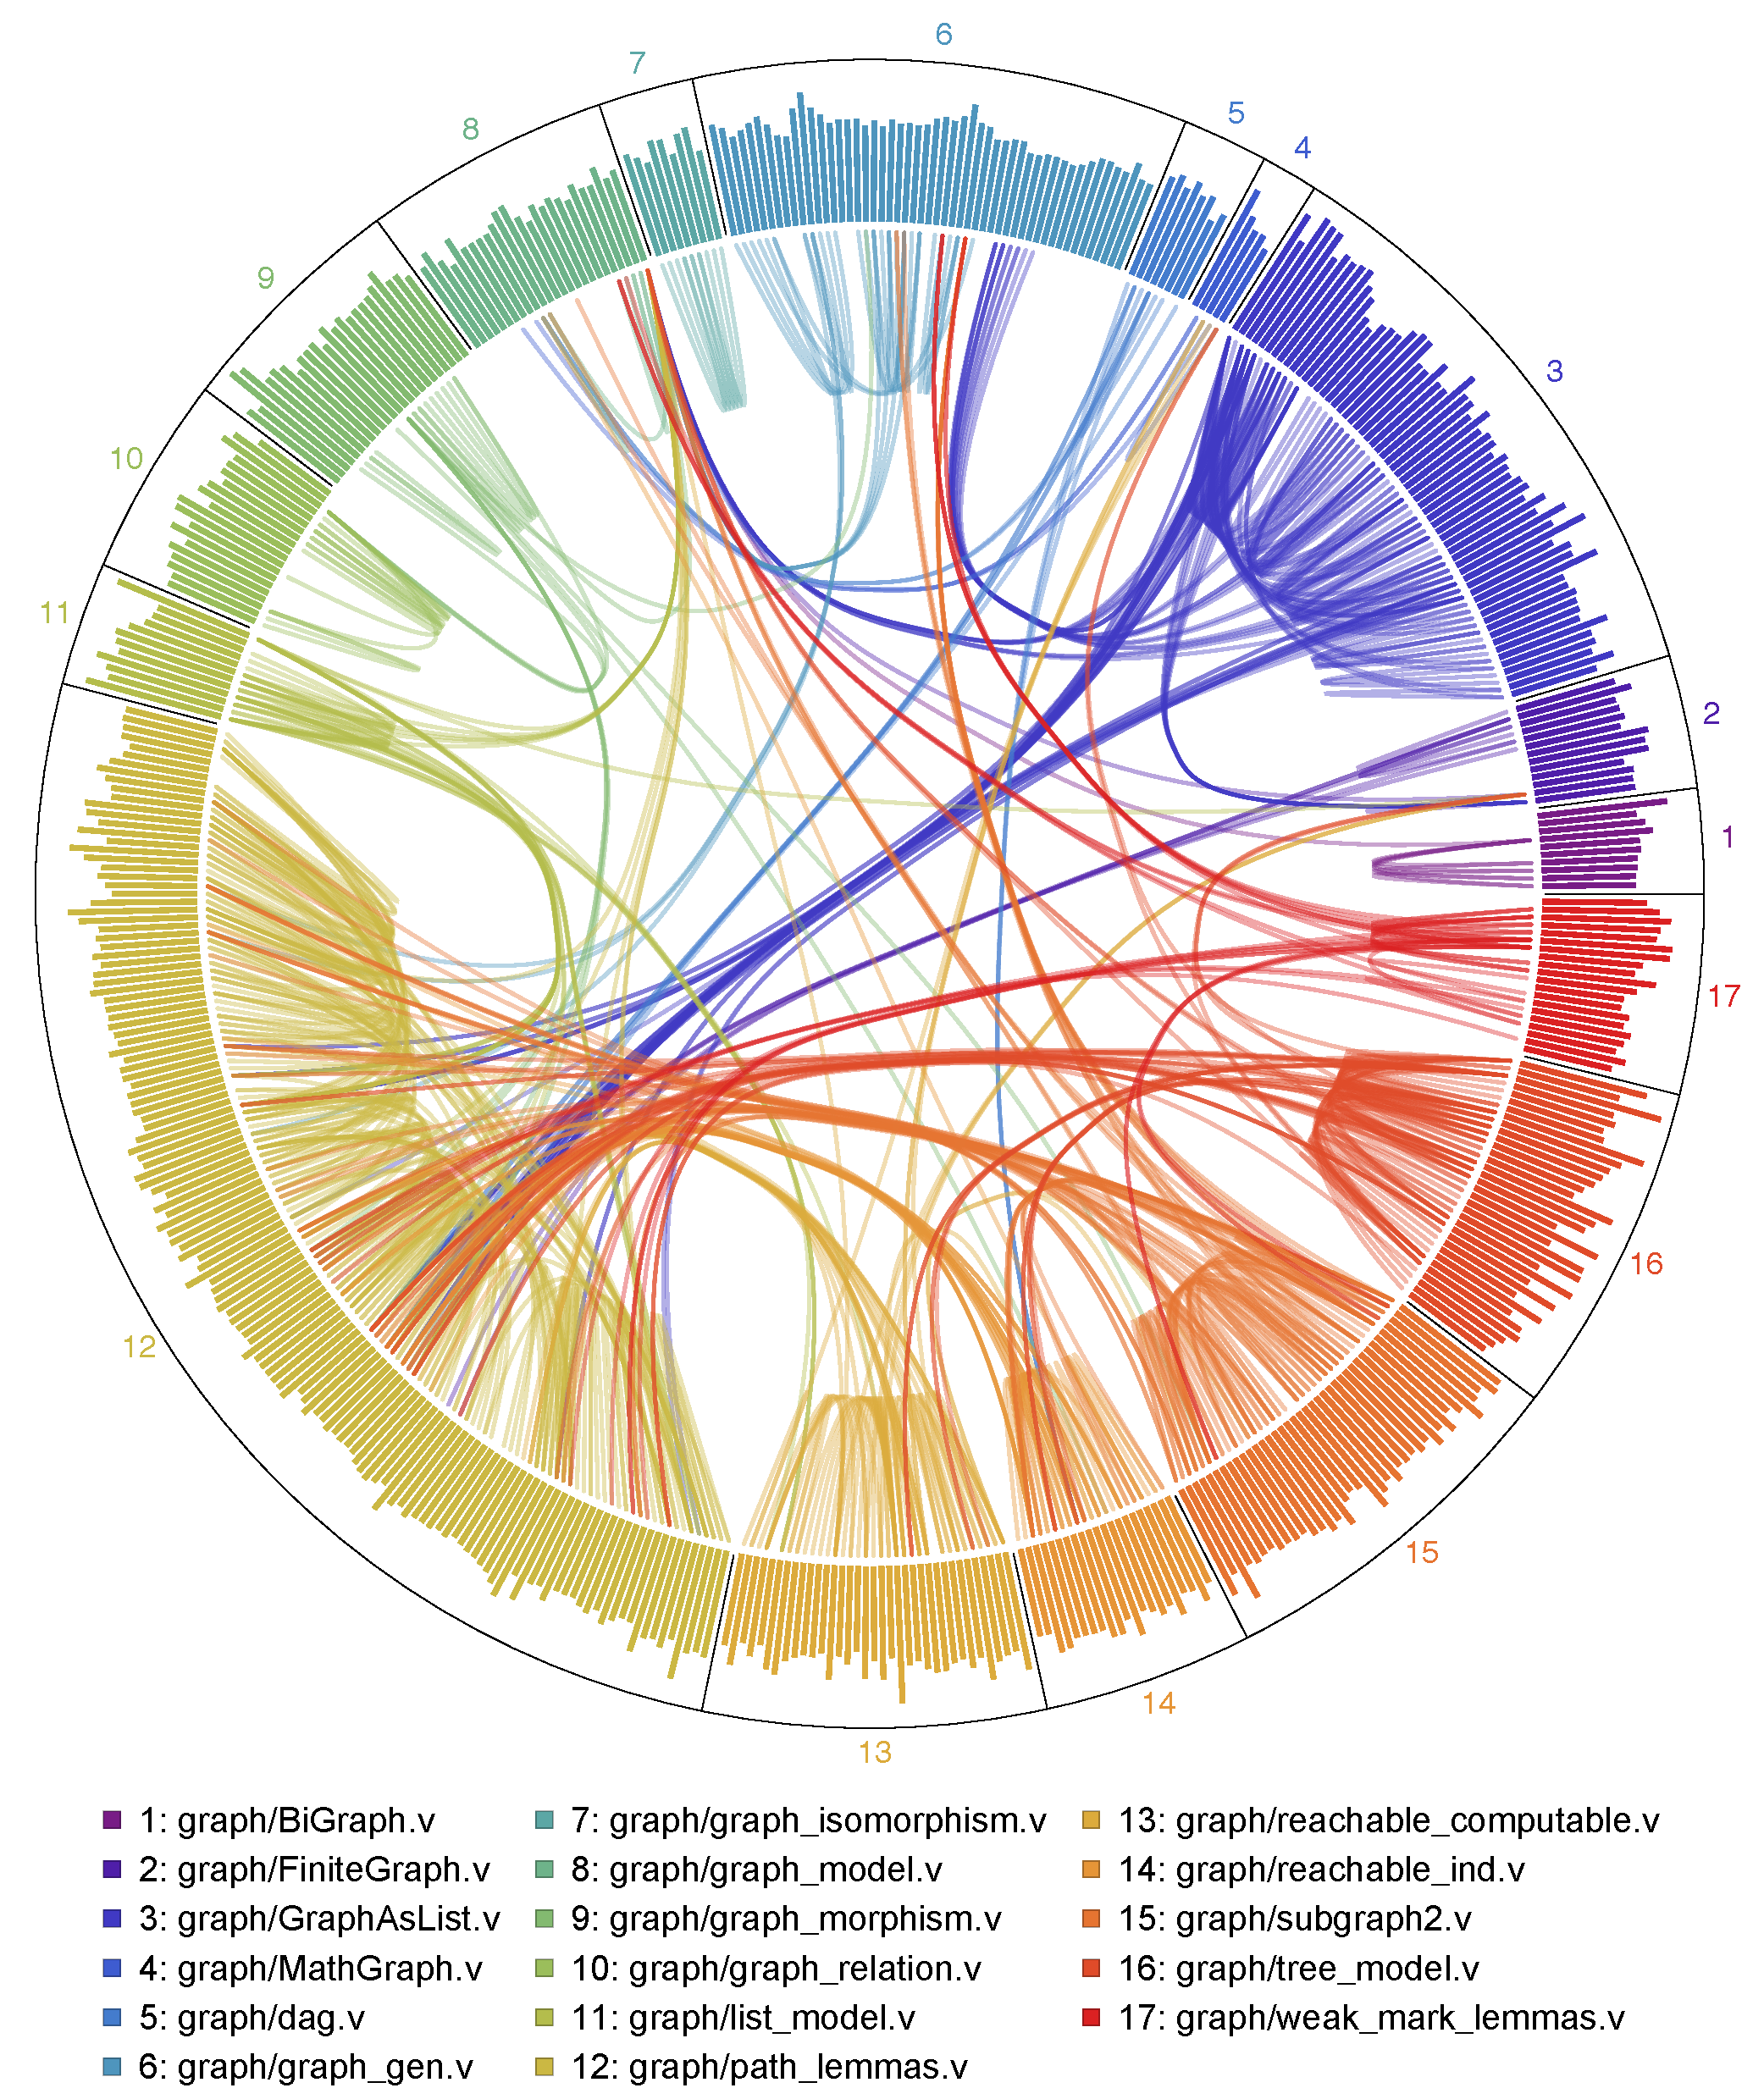
\includegraphics[width=0.75\textwidth]{mathgraph_theorems}
% 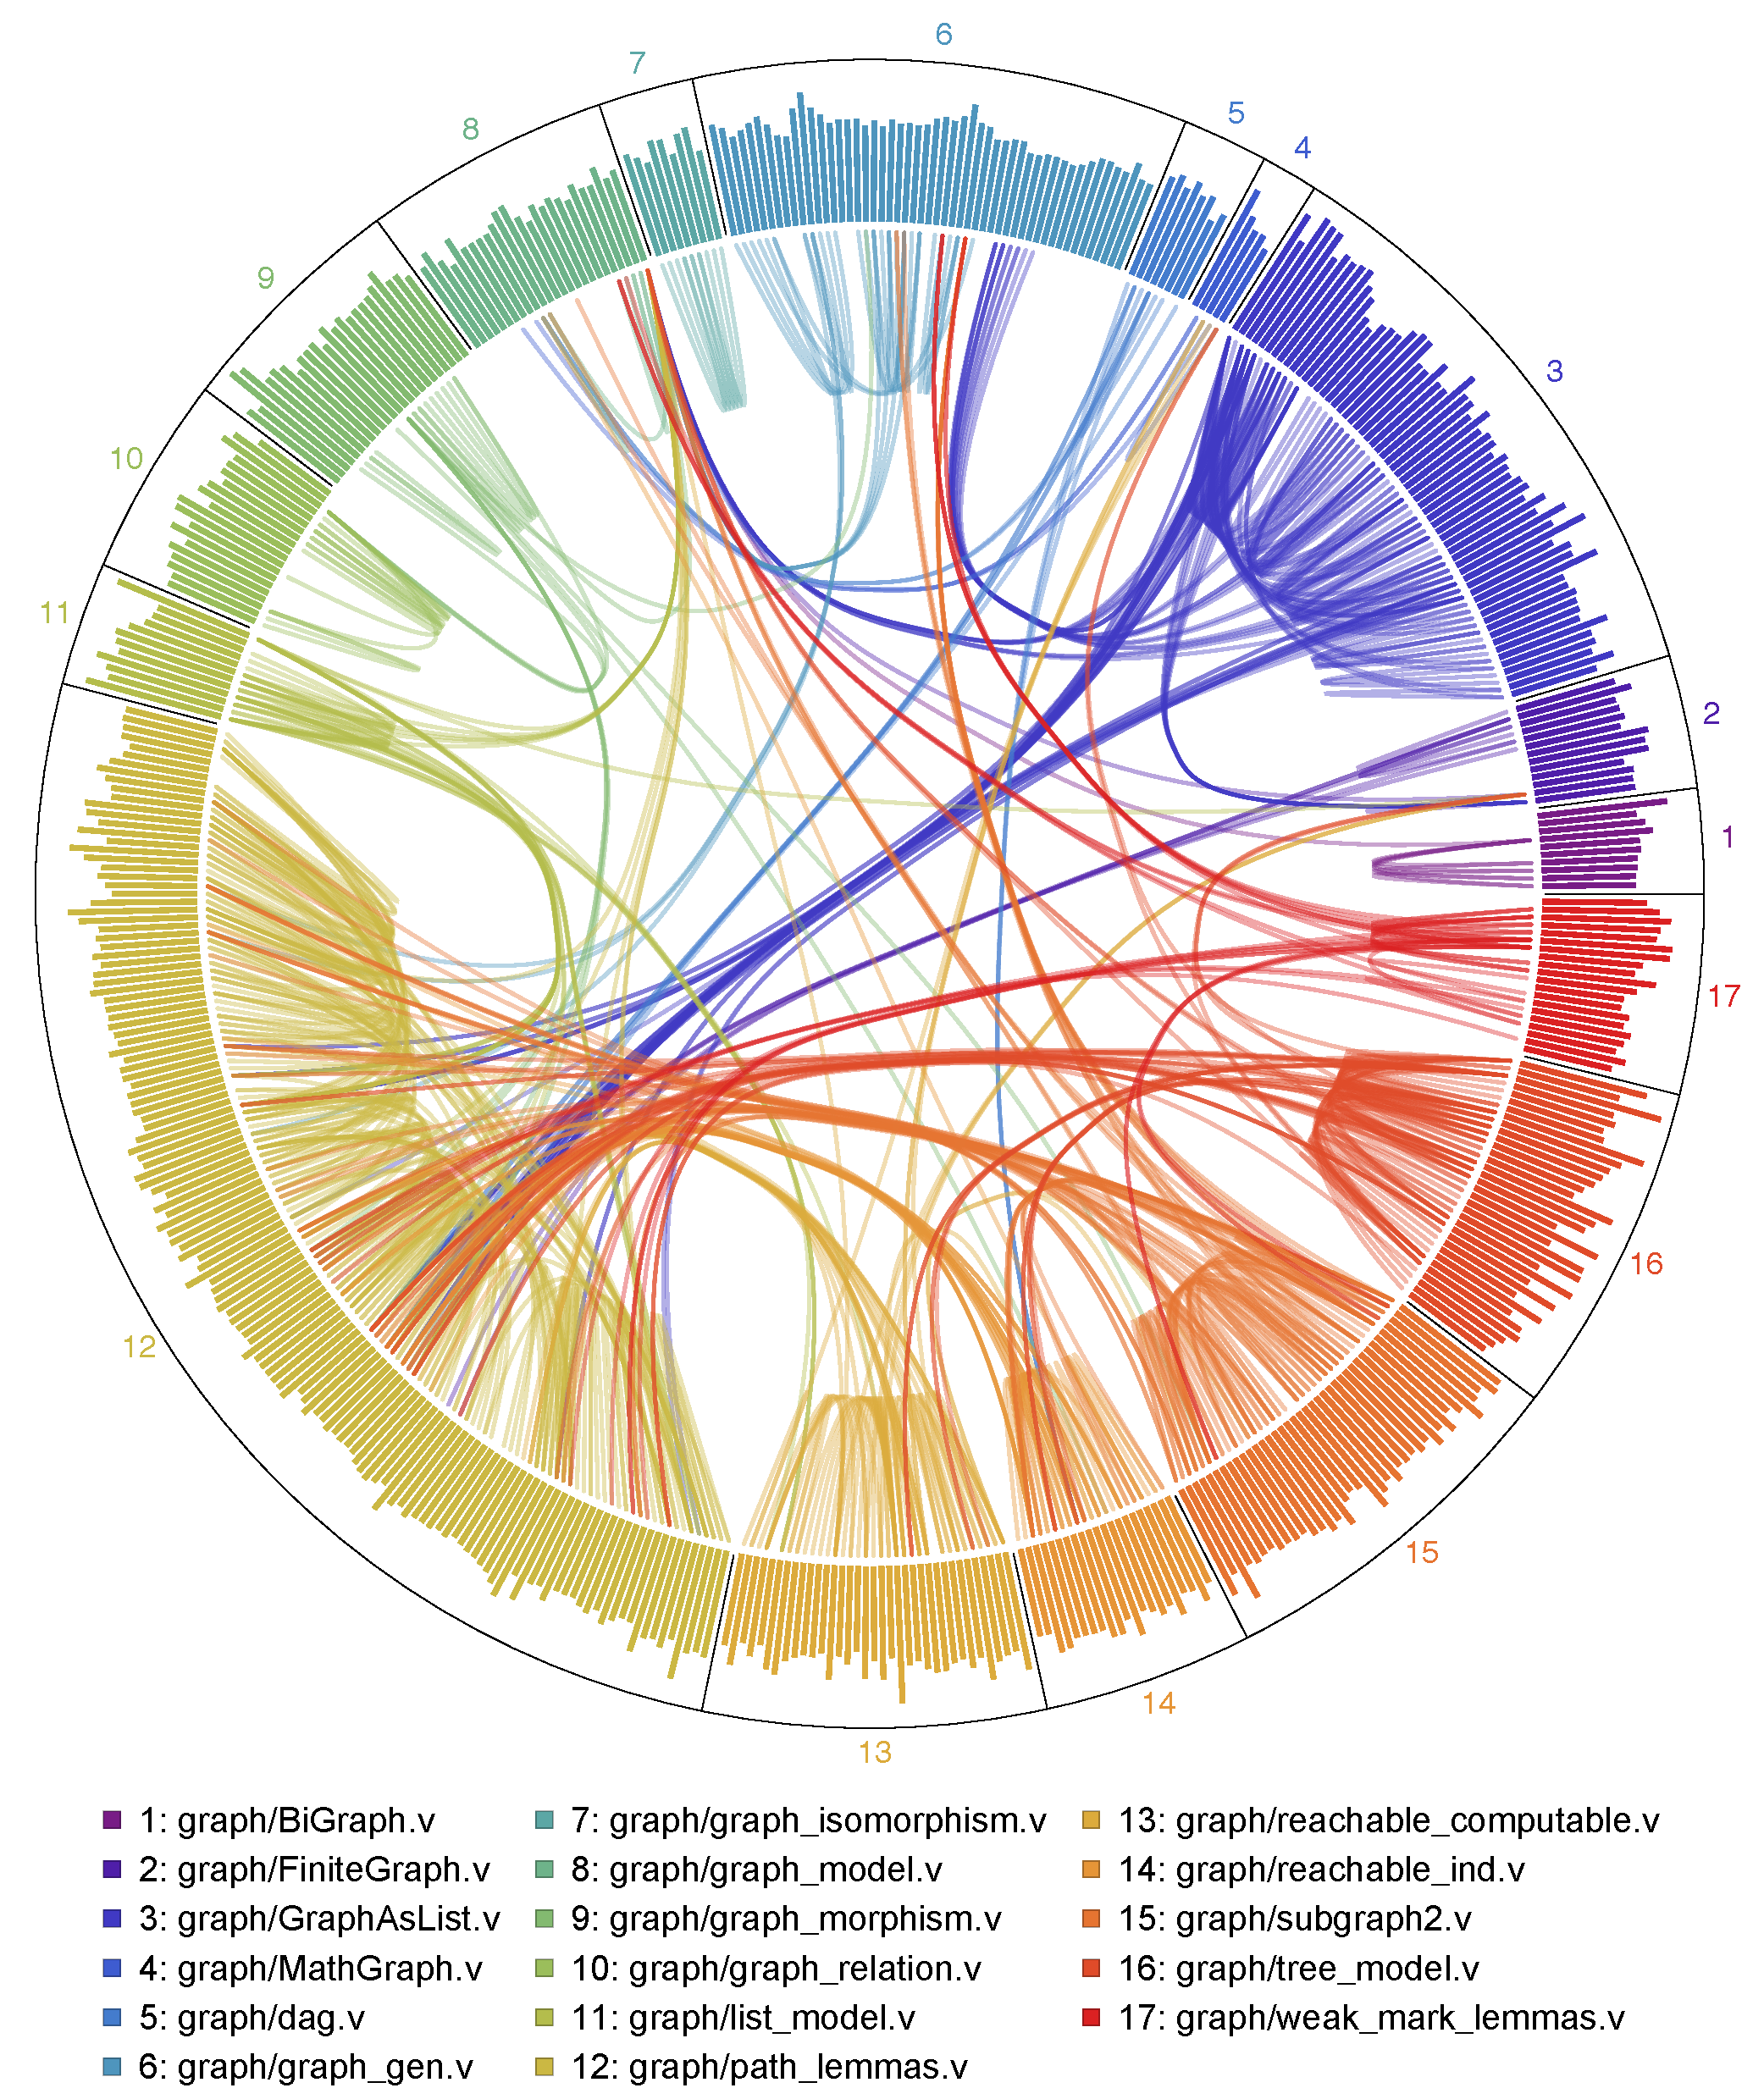
\includepdf[pages={1},scale=.5]{mathgraph_theorems.pdf}
\end{figure}

\begin{table}[b]
\centering
\begin{tabular}{c|c|c|c|c|c}
Component & Section & Files & Size (in lines) & Definitions & Theorems\\\hline
Common Utilities & & 10 & 3,578 & 44 & 289 \\
Math Graph Library & \S\ref{sec:mathgraph} & 20 & 10,585 & 216 & 581 \\
Spatial Graph Library & \S\ref{sec:spacegraph} & 3 & 2,328 & 59 & 110 \\
Integration into VST & \S\ref{sec:localizations},\S\ref{sec:development} & 11 & 2,783 & 17 & 172 \\
\hline
Marking (graph and DAG) & \S\ref{sec:localizations} & 6 & 775 & 9 & 20 \\
Spanning Tree & \S\ref{sec:localizations} & 5 & 2,723 & 17 & 92 \\
Union-Find (heap and array) & \S\ref{sec:orientation} & 18 & 3,193 & 107 & 135 \\
Garbage Collector & \S\ref{sec:certigc} & 16 & 13,858 & 235 & 712 \\
\hline & & & & & \\
[-2.2em] \\
\hline & & & & & \\
[-1em]
Total Development & & 89 & 39,823 & 704 & 2,111 \\
\end{tabular}
\caption{Statistics for our code base}
\label{tab:codebase}
\end{table}

All our results in this paper have been machine-checked.
%The bulk of our development was checked in Coq, although a 55-line file (shown in Figure~\ref{fig:hipmarkgraph}) was checked in HIP/SLEEK.  Our modifications to H/S itself were not machine-checked since H/S does not have a mechanized soundness proof.
Although the size of a development does not perfectly match with that development's importance or implementation difficulty, we present the size nonetheless in Table~\ref{tab:codebase}.
%, organized roughly by the paper section corresponding to each development.
Our proof script is written in a very
dense style.
For comparison, verifying a simple 39-line list-based merge sort in VST takes 600 lines.
At $\approx400$ LOC, the garbage collector is much larger, and is very complicated both
mathematically and spatially, in many places teetering on the edge of what can be defined
in~C.  For context, CompCert has 217k LOC, 5,687 definitions, and 6,694 theorems;
VST has 623k LOC, 14,038 definitions, and 21,442 theorems.

%It took fewer than 400 lines of Coq to verify the \li{mark} algorithm in H/S, indicating that a large portion of the codebase is shared between VST and H/S.  For context, VST and H/S have approximately 140k and 179k LOC.

\hide{
\paragraph{Size of Coq mathgraph \S\ref{sec:mathgraph}.}
Graph folder has 18 files in total with 10,919 lines in total

\paragraph{Size of Coq spacegraph \S\ref{sec:spacegraph}.}

not including the connection to H/S or VST

include \li{Graph.v} and \li{GraphBi.v} from \li{msl_application} since they do not depend on the underlying VST model?

What is in \li{ramification_lemmas}?  %Any other parts of VST ``standard'' from our work?

\paragraph{Integration into Floyd (\S\ref{sec:vst}).}: ?
Size of additions to VST logic model: ?

\paragraph{Modifications to HIP/SLEEK.}
H/S code: approximately 2,500 lines of code across 51 files
Size of extra H/S memory model:
\li{alg_seplog_direct.v}  52 lines
\li{overlapping_direct.v} 442 lines  {\color{magenta}How do we handle alignment?}
\li{precise_direct.v} 111 lines
other files?

\paragraph{Size of VST examples~\S\ref{sec:application}.}

Note: graph, graphbi (in space), graphmark, graphbimark are shared in \li{msl_application}

mark graph  19 + 402 + 161 + 246 = 828
mark dag  19 + 402 + 161 + 210
Note: mark dag shares 19 + 402 + 161 with mark graph

copy   459 + 19 + 161 + 388 = 1,027 (need to add files from \li{msl_applicatin})
dispose   475 + 18 + 544 = 1,037 (need to add files from \li{data_structure})
What do copy or dispose share with mark or with each other?

total: 1,038 (marks) + 2,064 (copy/dispose, assuming no duplication) = 3,102 lines.  12 files, assuming no sharing for copy/dispose (with each other or with mark)

\paragraph{Size of H/S example.}
main file: 54 lines (Figure~\ref{fig:hipmarkgraph}), \li{Module Type} generated by H/S (Figure~\ref{fig:hipcoqfile}) is 30 lines, Coq \li{Module} matching this \li{Module Type} is 358 lines.
total: 2 human-generated files, 429 lines

\paragraph{Size of total development.} ?
}


\section{Related work}
\label{sec:related}

\paragraph{Comparison with~\citet{hobor:ramification}.}
Our work builds on the theory of ramification by Hobor and Villard,
who verified graph algorithms on pen-and-paper using their \infrulestyle{Ramify} rule:
\begin{equation*}
%\label{eq:ramify}
\inferrule[Ramify]
{\{ L_1 \} ~ c ~ \{ L_2 \} \\
G_1 |- L_1 * (L_2 --* G_2)}
{\{ G_1 \} ~ c ~ \{ G_2 \}} \qquad \mathit{freevars}(L_2 --* G_2) \cap \MV(c) = \emptyset
\end{equation*}
Our \textsc{Localize} rule upgrades \textsc{Ramify} to better handle modified program
variables (note the side condition and recall the discussion in \S\ref{sec:localizations})
and existential quantifiers in postconditions.  Hobor and Villard avoided these challenges
by proposing a unwieldy variant of \infrulestyle{Ramify} called \infrulestyle{RamifyAssign}, which
could reason about the special case of a single assignment $\li{x=}f(\ldots)$, assuming
the verifier can make the local program translation to $\li{x'=}f(\ldots)\li{; x=x'}$,
where \li{x'} is fresh.  This is nontrivial in large existing formal
developments, such as VST, that do not have any way to prove programs equivalent.
Hobor and Villard could not verify unmodified program code, modify program variables
inside nested localization blocks, or handle multiple assignments in a single block as
in lines~\ref{code:markbeforetripleramify}--\ref{code:markaftertripleramify} of
Figure~\ref{fig:markgraph}.  They avoided existentials in localized
postconditions by defining all mathematical operations (\emph{e.g.} $\m{mark}$) as
functions rather than as relations; this is fine for pen-and-paper, but painful in
a mechanized setting wherein functions must be proven to terminate.

Hobor and Villard treated mathematical graphs as triples $(V,E,L)$ of
vertices, edges, and a vertex labeling function, where vertices had no more than two
neighbors. Our mathematical graph framework~(\S\ref{sec:mathgraph}) is more
modular and versatile, and ships with hundreds of reusable definitions and theorems. Further, our library has been tuned to work smoothly in a mechanized context.


Hobor and Villard erroneously defined spatial graphs
recursively. Unfortunately, other members of the research
community (\emph{e.g.}~\citet{raadvg15}) followed their lead.  We expose this
error~(\S\ref{sec:fixpointfail}) and provide a sound and rather general definition for
\p{graph} that recovers fold/unfold reasoning~(\S\ref{sec:goodgraph}).  We develop a
much more general and more modular set of related lemmas and connected our spatial
reasoning to the verification framework of CompCert/VST~(\S\ref{sec:vst}).
Our development is entirely
machine-checked~(\S\ref{sec:development}) whereas they used only pen and paper.

\paragraph{Other pen-and-paper verification of graph algorithms and/or $**$.}

\citet{hongseok:phd} verified the Schorr-Waite algorithm, and this 
is widely considered a landmark in the early separation logic literature. 
\citet{bornat:aliasing04}~gave an early attempt to reason about graph algorithms 
in separation logic in a more general way. 
\citet{neelthesis}~provided the first separation logic proof of union-find.

\citet{rey-slnotes}~was the first to document the overlapping 
conjunction $**$, albeit without any strategy to reason about it using Hoare rules. 
\citet{gardnerms12}~were the first to reason about a program using $**$ in 
Javascript. 
\citet{raadvg15}~used $**$ within their CoLoSL program logic to reason about 
a concurrent spanning algorithm using a kind of ``concurrent localization''.

%\paragraph{Alternative fixpoint constructions.}
%Appel and McAllester defined an alternative ``contractive'' fixpoint that is sometimes used to define recursive predicates in separation
%logic~\cite{appel:fixpoint}.  In Appendix~\ref{apx:appelfixpiont} we explain why Appel and McAllester's  is also unsuitable to define graphs.

\paragraph{Machine-checked verification of graph algorithms.}
A decade after Yang verified Schorr-Waite on paper, \citet{leino10} automated 
its verification in Dafny. 
\citet{ilya-graphs}~verified a concurrent spanning tree algorithm, and 
moreover developed mechanized Coq proofs. Their algorithm was written in FCSL, 
a monadic DSL that combines effectful operations with pure Coq expressions; 
FSCL cannot be executed. 
\citet{chen18}~compared how three provers (Coq, Isabelle, and Why3) can 
verify Tarjan’s strongly-connected component algorithm written in the native 
language of each of the tools. Because these are written in the native languages 
of a proof assistant, they avoid “real-world” language concerns such as 
memory models and overflow.

\citet{lamneu15}~extended the Isabelle Refinement Framework to verify a range of 
DFS algorithms via stepwise refinement.
Their framework allows the reuse of previously-proved DFS 
invariants by establishing an inductive
``most specific invariant'' and deriving other inductive invariants from it.
\citet{lamsef19}~extended this further and presented verifications of 
the correctness and time complexity of the Edmonds-Karp and push-relabel
algorithms. Lammich et al. produced very readable proofs of classic 
textbook algorithms by using the Isar language atop their Isabelle proofs.
They used Isabelle's code generator to export efficient executable code, 
but with the caveat that the code comes with a guarantee of only 
partial correctness semantics.

\citet{char11}~used his CFML tool to Coq-verify an OCaml implementation of 
Dijkstra. 
\citet{gueneauetal19}~extended CFML and verified the correctness 
and time complexity of a modified version of the BFGT cycle-detection algorithm.
The graph algorithms verified in CFML tend to be ``graph theory'' in flavour, 
whereas the algorithms we have verified tend to have more of a
``systems'' flavor. This difference is partially explained by the fact that 
code written in ML can take advantage of its high-level design, whereas
code written in C is often interested in handling grungy systems tasks. For 
example, references in ML cannot be null and do not support pointer arithmetic; 
of course both are possible---and lead to nontrivial complications---in 
C. Accordingly, the CFML proofs benefit from ML’s cleaner computational model. 
Our verifications are in C so we must contend with C’s memory model, pointer 
arithmetic, significant scope for undefined behavior, and so forth.

\citet{charpott15, charpott19}~used CFML to verify the correctness and 
time complexity of union-find. Their work is an interesting counterpoint to 
ours because, while it maintains an abstraction between the client and the 
internal mathematical/spatial facts that the client need not know, it does 
not maintain a separation between the mathematical and spatial 
facts themselves, as we do in~\S\ref{sec:mathgraph} and ~\S\ref{sec:spacegraph}.
This separation is worthwhile: our modular method let us verify an alternate 
version of union-find that uses an array of vertices rather than individually 
heap-allocated nodes. This 
secondary verification then used \emph{exactly the same} mathematical proof of 
functional correctness despite the radically different layout of spatial 
memory.
Our work does not verify the time complexity of union-find. When 
we attempted to prove the necessary amortisation bounds we ran into an 
overflow issue: it was impossible to prove that the rank would not exceed 
\li{max\_int} because the CompCert memory model does not place a bound on the 
total number of allocations. Informally, this overflow is impossible in 
practice because no computer has $2^{2^{\tiny 64}}$ bytes of memory, which would 
be required for this overflow to occur, but Coq remains unconvinced. 
Chargu{\'{e}}raud and Pottier acknowledged and sidestepped this issue by 
representing rank using the Coq type \li{Z}, which was not an option for us 
given the end-to-end nature of the VST+CompCert toolchain.

\paragraph{Verification tools in Coq.}
Our work interacts with the Floyd verification module within the Verified 
Software Toolchain (VST)~\cite{appel:programlogics}. The Floyd module uses 
tactics to enable the separation-logic verification of CompCert C programs. 
VST connects to the CompCert certified C compiler~\cite{leroy:compcert}, and 
thus has no gaps or admits between the verified source code and the eventual
assembly code~\cite{appelvst}.

Charge! likewise uses Coq tactics to work with a shallow embedding of higher 
order separation logic, but focuses on OO programs written in 
Java/C\#~~\cite{bengtson:charge}. Iris Proof Mode provides a similar framework 
for higher-order concurrent reasoning in Coq~\cite{krebbers:iris}.

CFML enables the verification of OCaml programs by reasoning about their
``characteristic formulae'' in separation logic using Coq~\cite{char10, char11}. 
CFML has been used to verify a range of functional and imperative programs,
including some graph-related algorithms as discussed 
above. \citet{charpott15, charpott19}~extended CFML to reason about time 
credits. The work of \citet{gueneau17}~indicates that CFML is exploring a connection 
with the certified CakeML compiler~\cite{cakeml}.

While the tools above require substantial human guidance, 
Bedrock~\cite{chlipala:bedrock} is a more automated approach to the verification of 
low level programs using separation logic in Coq. 
Bedrock leverages the fact that phrasing function 
specifications in a \emph{computational} style 
(in this case, inspired by functional programming) 
leads to separation logic proof obligations that are quite automatable.
It simplifies these obligations into pure mathematics using a 
custom workhorse tactic, and then discharges those 
obligations using standard Coq automation.

\paragraph{Other verification tools.} 

Many more-automated verification tools also use separation logic in a forward
reasoning style. Smallfoot~\cite{berdine:smallfoot}, jStar~~\cite{distefanop08}, 
HIP/SLEEK~\cite{chin:hipsleek}, and Verifast~\cite{jacobs:verifast} are landmarks
at various points on the expressibility-automatability spectrum. 
KeY~\cite{beckert:2007} and Dafny~\cite{leino10} are verifiers that are not 
based on separation logic. KeY uses an interactive verifier while Dafny pursues
 automation with Z3~\cite{moura2008}.

\paragraph{Mechanized mathematical graph theory.}
There is a long history, going back at least 28 years, of mechanized 
reasoning about mathematical graphs~\cite{wong1991}. 
The most famous mechanically verified “graph theorem” is the Four Color 
Theorem~\cite{gonthier2005computer}; however the development actually uses
hypermaps instead of graphs. In general most “mathematical graph” frameworks in 
the literature~\cite{wong1991, chou1994, yamamoto1995formalization, rwpgt1998, yamamoto1998formalization, tamai2000formal, duprat2001coq, ridge2005graphs, nipkow2016, dijkstra_shortest_path-afp} were not used to verify real 
code, for which they seem unsuitable. Verifying real code requires delicate concepts such as removing a subgraph, null nodes, and parallel edges, and one of our contributions is that our framework is general enough to support such verification. 
\citet{noschinski2015}~built a graph library in Isabelle/HOL whose formalization 
is the closest to ours, 
\emph{e.g.} supporting graphs with labeled and parallel arcs. 
Beyond being in Coq, our setup supports at least three features beyond 
Noschinski’s: reasoning about incomplete graphs (as discussed 
in~\S\ref{sec:mathinfra} using figure~\ref{fig:pregraph}), labeling the graph 
as a whole (used, for example, in the garbage collector to store 
metainformation about the number and location of the generations), and our 
modular typeclass-supported “graphs with properties” setup in General Graph 
(as described in~\S\ref{subsec:graphplugins}). 
\citet{dubois2015graphes} and \citet{noschinski2015formalizing}~used proof assistants to 
design verifiable checkers for solutions to graph problems. 
\citet{bauer20025} and \citet{yamamoto1995formalization}~used an inductive encoding of graphs to formalize planar graph theory.


\paragraph{Verification of garbage collection algorithms.}
Schism \cite{gcexample4,gcexample4a} is a certified concurrent
collector built in a Java VM that services multi-core architectures with weak memory consistency.
\citet{gcexample5, gcexample3} introduced GCminor, which is
a certified translation step added to CompCert's translation from Clight to assembly.
GCminor makes explicit the specific invariants that the garbage collector
relies upon, thus minimising errors due to the violation of invariants
between the garbage collector and the mutator.
\citet{gcexample2} annotated x86 code
for two GCs by hand, and then used Boogie and the Z3 automated theorem prover
to verify their correctness automatically.

The closest piece of work to our certified GC is probably the excellent certified GC
for the Cake ML project~\cite{cakemlgc}, since both integrate a certified GC into 
a certified compiler for a functional language.  Their GC is written closer to assembly 
than C, which is both a positive---in that they avoid undefined behaviors---and a negative, 
in that their GC is harder to understand and upgrade and cannot take advantage of the
mature CompCert compiler.  Their GC lacks some of our optimisations (\emph{e.g.} they have 
only three generations), but on the other hand handles mutation in the GC heap.  The largest 
difference, however, is that we present an integrated graph framework suitable for reasoning 
about many graph algorithms, of which our GC is merely the flagship.  In contrast, they focus 
much more narrowly on the problem of certified GCs.


\section{Future work and conclusion}
\label{sec:future}
\label{sec:conclusion}
In the future we plan to improve the pure reasoning of graphs and
similar data structures.  {\color{magenta}We are in the process of verifying a garbage
collector for the ``CertiCoq'' project, which is building
a certified compiler from Gallina to Clight. We would like to investigate
using our externally verified lemmas in HIP/SLEEK to verify code such as fast
exponentiation and more graph algorithms. We also would like to make
the interface between Coq and H/S simpler and cleaner.
One final direction we would like to investigate is using our new
connection to Coq to have H/S output certificates as it
verifies programs so that the system becomes more trustworthy.}

Our main contributions were as follows.  We connected our reasoning
to a real-world verification tool and used it to verify several graph-manipulating algorithms.
We generalized the \infrulestyle{Ramify}
rule to handle modified program variables and existential quantifiers in postconditions
more smoothly.  We developed a general and modular framework for reasoning
about mathematical graphs and a general and modular spatial library for
reasoning about graphs in the heap.  We gave a sound definition for \p{graph}
that still enjoys fold/unfold. We reported on the certification of a GC... . We found two places where the C semantics are too weak... .


%\vfill
%\pagebreak


%\paragraph{Acknowledgements.} This material was based in part on research supported by Yale-NUS College and R-607-265-045-121.  All opinions expressed in this work are solely those of the authors.
%
%This material is based in part on research sponsored by DARPA under agreement number
%FA8750-12-2-0293. The U.S. Government is authorized to reproduce
%and distribute reprints for Governmental purposes notwithstanding
%any copyright notation thereon. The views and conclusions contained
%herein are those of the authors and should not be interpreted as
%necessarily representing the official policies or endorsements,
%either expressed or implied, of DARPA or the U.S. Government.

\bibliographystyle{abbrvnat}
%\bibliographystyle{tropbien_nopages}
\bibliography{autoquack}

%% Appendix
\appendix
\section{Appendix}

%
\appendix

{\color{magenta}
\section{Simplifying ramification entailments}
After applying \infrulestyle{Solve Ramify-PQ}, it is often desirable to break the ramification entailment into smaller disjoint pieces before trying to solve it directly.
One common case is to ``frame out'' an unneeded part of the global state:
\[
\infrule{Frame Ramify-Q}
{G_1 \vdash L_1 * \forall x.~ (L_2 --* G_2)}  
{G_1 * F \vdash L_1 * \forall x.~ \big(L_2 --* (G_2 * F)\big) }
{\begin{array}{c}F \text{ ignores} \\ \MV(c) \cup \{x\} \end{array}} \qquad \qquad \qquad
\]
In fact \infrulestyle{Frame Ramify-Q} is a consequence of the more general \[
\infrule{Split Ramify-Q}
{G_1 \vdash L_1 * \big(\forall x.~ (L_2 --* G_2)\big) \! \! \! \! \\
 G_1' \vdash L_1' * \big(\forall x.~ (L_2' --* G_2')\big) }
{G_1 * G_1' \vdash L_1 * L_1' * \Big(\forall x.~ \big((L_2 * L_2') --* (G_2 * G_2')\big)\Big)} {}
\]
In general the strategy is to apply \infrulestyle{Frame Ramify-P} and \infrulestyle{Split Ramify-P} until the ramification entailments are as small as they can be (while remaining true!) before using \infrulestyle{Solve Ramify-P} on the remaining ``atoms''.

The situation is unfortunately a little messier when the postconditions contain existential quantifiers.

\[\text{UNSOUND-RAM-Q-SPLIT}\]
\Rule{}
{G_1 \vdash L_1 * (\exists x, L_1' (x) --* \exists x, G_1'(x)) \\
G_2 \vdash L_2 * (\exists x, L_2' (x) --* \exists x, G_2'(x)) \\}
{G_1 * G_2 \vdash L_1 * L_2 * (\exists x, L_1'(x) * L_2'(x) --* \exists x, G_1'(x) * G_2'(x)) }


\[
\infrule{Ramify-Q}
{\{ L \} ~ c ~ \{\exists x.~ L' \} \\
 G \vdash L * \big(\forall x.~ (L' --* G')\big)}
{\{ G \} ~ c ~ \{ \exists x.~G' \}}{}
\]

}


\section{Junk}
{\color{magenta} Universally-quantified metavariables can appear free in the predicates to make further connections.
Assuming that the abstracted pre- and postconditions $A$, $B$, $C$, and $D$ above all use \li{x}, we proceed
as follows.  First we introduce a new fresh metavariable $x$ whose value will be equal to \li{x} after the localization, and then choose $F \stackrel{\Delta}{=} [\li{x} |-> x] (C -* D)$, that is we substitute the program
variable \li{x} for the metavariable $x$.  Since we have substituted away \li{x}, $F$ ignores it and so we satisfy the side condition on \infrulestyle{Solve Ramify-P}.  We then must strengthen $C$ into $C' \stackrel{\Delta}{=} C /| \li{x} = x$ to make the connection at the appropriate program point.  Now we are left with the entailments
\[
\begin{array}{lcl}
\li{x} = 5 /| A & |- & (\li{x} = 5 /| B) * F \\
F & |- & (\li{x} = 6 /| C') -* (x = 6 /| D)
\end{array}
\]
To further relate the earlier and later values of \li{x} in $F$ we can introduce a second fresh $x'$ and use $B' \stackrel{\Delta}{=} B /| \li{x} = x'$.
}

The \infrulestyle{Ramify} rule is sound but interacts poorly with modified program variables (as in lines~\ref{code:markbeforetripleramify}--\ref{code:markaftertripleramify} of Figure~\ref{fig:markgraph}) {\color{magenta} and
localized existentials (as in lines~\ref{code:beforemarkl}--\ref{code:aftermarkl})}.  Both of these limitations are annoying enough in paper proofs and graduate to major headaches in mechanized ones.  Happily, we show how to overcome both limitations in \S\ref{sec:freevars} and \S\ref{sec:existentials}, respectively, by presenting new variants of \infrulestyle{Ramify}.  Our notation carries over without significant change: just use the new rules to enable the more general ramification entailments they permit.
%When in doubt the most general rule, \infrulestyle{Ramify-PQ} from \S\ref{sec:existentials}, implies all of the others.

\section{More junk}
\hide{
\section{Ramification Rules}


\Rule{Frame  }
{\{ P \} c \{Q \} \\
  F \text{ is stable w.r.t. } \MV(c)\\}
 {\{P * F \} c \{ Q * F \}}

\Rule{Ramification   }
{\{ L \} c \{L' \} \\
 G \vdash L * (L' -* G') \\
 (L' -* G') \text{ is stable w.r.t. } \MV(c)\\}
{\{ G \} c \{ G' \}}

\Rule{Ramification-P }
{\{ L \} c \{L' \} \\
 G \vdash L * \Box^{\llbracket c \rrbracket} (L' -* G') \\}
{\{ G \} c \{ G' \}}

\subsection{P for Pure Facts}

Separation logic has been mechanized by many projects CITE CITE CITE.
In many of them, like VST and Charge!, expressing the value of a local
variable (a variable stored in stack) is a pure fact rather than a
spatial fact. Because the side condition of ramification rule requires $(L' -* G')$ to be stable w.r.t. modified local variables in $c$\footnote{In previous papers, the side conditions of Frame rule and ramification rule are usually expressed as ``$\FV(F) \cap \MV(c) = \emptyset$'' and ``$\FV(L' -* G') \cap \MV(c) = \emptyset$''. The side conditions used in this paper are equivalent with typical ones if the semantic interpretation of $\FV$ is used. All the previous mentioned projects takes semantic interpretation instead of syntactical interpretation.}, it is almost impossible to apply ramification rule in any practical situations in these systems. In this paper, we present a pure-facts-related rule (we call it ramification-P rule, or just P rule, in the rest of this paper) such that it is sound and practical in the most general setting of separation logics.

The primary ramification rule is essentially an application of the frame rule using $(L' -* G')$ as frame.
Thus, the key point of handling pure facts is to find a legal frame even if $(L' -* G')$ is not stable w.r.t. $\MV(c)$. This frame is $\Box^{\llbracket c \rrbracket} (L' -* G')$ in ramification-P rule.
\begin{eqnarray*}
m \models \Box^R P &  \Leftrightarrow  & \forall m', \text{ if } m\xrightarrow{R}m' \text{ then } m' \models P \\
m \xrightarrow{\llbracket c \rrbracket} m' & \Leftrightarrow &   \text{$m$ and $m'$ coincide everywhere} \\
&& \text{except $\MV(c)$} \\
P \text{ is stable} &  \Leftrightarrow  & \forall m \ m',  \text{if $m$ and $m'$ coincide everywhere} \\
\text{w.r.t. $S$} && \text{except $S$, then $m \models P$ iff $m' \models P$}
\end{eqnarray*}

Here, $\Box$ represents the necessity modal operator. The formula $\Box^{\llbracket c \rrbracket} (L' -* G')$ says, it is true on a state $m$ if and only if for any state $m'$, if $m$ and $m'$
coincide everywhere except on the variables modified by $c$, then $(L' -* G')$ is true on $m'$.

Based on the combination frame rule, consequence rule and three basic facts below, we can immediate prove ramification-P rule.
\begin{quotation}
(a) $\Box^{\llbracket c \rrbracket} (L' -* G')$ is stable w.r.t. $\MV(c).$\footnote{This can be proved directly from the definition of $\llbracket c \rrbracket$ and stability, and the fact that $\llbracket c \rrbracket$ is an equivalence relation.}

(b) $G \vdash L * \Box^{\llbracket c \rrbracket} (L' -* G')$. (Assumption)

(c) $L' *  \Box^{\llbracket c \rrbracket} (L' -* G') \vdash G'$. \footnote{When $R$ is reflexive, T-Axiom of modal logic is sound, i.e. for any $P$, $\Box^R P \vdash P$. As $\llbracket c \rrbracket$ is reflexive, we know the fact that $\Box^{\llbracket c \rrbracket} (L' -* G') \vdash L' -* G'$, which is immediate followed by $L' *  \Box^{\llbracket c \rrbracket (L' -* G')} \vdash G'$.}
\end{quotation}

\subsection{Establish the Assumption Entailment of P Rule}

It is well-known that the proof theory with magic wand is already complicated, so generally speaking, it will not be a easy task to prove an entailment with magic wand together with modality. However, people need to prove an entailment with form
\begin{equation}G \vdash  L * \Box^R (L' -* G') \label{eqn:Passu} \end{equation}
at first when applying ramification-P rule. Luckily, this special form makes the task simpler.

First of all, SOLVE-RAM-P rule can turn the proof goal into two wand-free and modality-free entailments. Specifically, people only need to find an $R$-stable predicate $F$, such that $G \vdash L * F$ and $F * L' \vdash G'$ are both true.

SOLVE-RAM-P alone is not a satisfactory proof theory because in that case using P rule would have no different from using frame rule directly. The key point here is that, an entailment with form \ref{Passu} can be proved in a modularized way. For primary ramification rule, CITE proposed two proof rule, RAM-FRAME and RAM-SPLIT\footnote{\Rule{RAM-FRAME }
{G \vdash L * (L' -* G') \\
F \text{ is stable w.r.t. } \MV(c) \\}
{G * F \vdash L * (L' -* G' * F) }

\Rule{RAM-SPLIT }
{G_1 \vdash L_1 * (L_1' -* G_1') \\
G_2 \vdash L_2 * (L_2' -* G_2') \\}
{G_1 * G_2 \vdash L_1 * L_2 * (L_1' * L_2' -* G_1' * G_2') }
}, to divide an entailment with form $G \vdash L * (L' -* G')$ into small pieces. When it comes to ramification-P rule, two corresponding proof rules, RAM-P-FRAME and RAM-P-SPLIT are still sound.

\Rule{SOLVE-RAM-P }
{G \vdash L * F\\
F * L' \vdash G' \\
F \text{ is stable w.r.t. } \MV(c) \\}
{G \vdash L * \Box^{\llbracket c \rrbracket} (L' -* G') }

\Rule{RAM-P-FRAME }
{G \vdash L * \Box^{\llbracket c \rrbracket} (L' -* G') \\
F \text{ is stable w.r.t. } \MV(c) \\}
{G * F \vdash L * \Box^{\llbracket c \rrbracket} (L' -* G' * F) }

\Rule{RAM-P-SPLIT }
{G_1 \vdash L_1 * \Box^{\llbracket c \rrbracket} (L_1' -* G_1') \\
G_2 \vdash L_2 * \Box^{\llbracket c \rrbracket} (L_2' -* G_2') \\}
{G_1 * G_2 \vdash L_1 * L_2 * \Box^{\llbracket c \rrbracket} (L_1' * L_2' -* G_1' * G_2') }

To conclude, if $L'$ and $G'$ are two separating conjunctions of a bunch of atomic predicates, RAM-P-FRAME and RAM-P-SPLIT can establish \ref{Passu} from entailments with the same form but smaller size. Atomic sized entailments can be proved using SOLVE-RAM-P. They are usually general purposed entailments and do not need to be proved for every single program. In section \ref{vst}, we will see examples of this approach for real programs.

\subsection{Q for Quantifiers}

In secion ???, we have already seen that it is a practical approach writing pre/postconditions as a separating conjunction of a list of atomic predicates (which makes RAM-P-FRAME and RAM-P-SPLIT useful). But unfortunately, an existential in post condition (also very common as we have seen in section ???) will prevent us from using these two rules. Now, one natural solution is to find other proof rules, like the following one, to deal with existential quantifiers.
\[\text{UNSOUND-RAM-Q-SPLIT}\]
\Rule{}
{G_1 \vdash L_1 * (\exists x, L_1' (x) -* \exists x, G_1'(x)) \\
G_2 \vdash L_2 * (\exists x, L_2' (x) -* \exists x, G_2'(x)) \\}
{G_1 * G_2 \vdash L_1 * L_2 * (\exists x, L_1'(x) * L_2'(x) -* \exists x, G_1'(x) * G_2'(x)) }

But this rule is NOT sound (even though we have not add $\Box$ operator to deal with local variable related stuff). The reason is that, given the local piece of memory satisfies $L_1'(x) * L_2'(x)$ for some specific $x$, we know that it can be split into two small piece of memory and they satisfies $L_1'(x)$ and $L_2'(x)$ respectively. Then the assumption tell us that the global piece can be split into two corresponding piece, $G_1'(x_1)$ and $G_2'(x_2)$ are true on them for some specific $x_1$ and $x_2$. Now the problem comes. Only if we could prove $x_1 = x_2$, we could prove the conclusion. But we cannot.

The key point of the failure above is that the frame, $\exists x, L' (x) -* \exists x, G'(x)$, says if $L'(x)$ is true on local then there is another (might be same one) $x_0$ such that $G'(x_0)$ is true on global. This is too weak for modularity. In many practical cases, we can in fact prove that $G'(x)$ should be true for the exact same $x$. This observation brings us to the ramification-PQ rule here.
\Rule{Ramification-PQ}
{\{ L \} c \{ \exists x, L' (x) \} \\
 G \vdash L * \Box^{\llbracket c \rrbracket} (\forall x, L' (x) -* G' (x)) \\}
{\{ G \} c \{ \exists x, G' (x)\}}

PQ rule can be directly derived from P rule by using the following theorem from separation logic\footnote{
$$\frac{\frac{\frac{\forall x, (L' (x) -* G' (x)) \vdash L' (x_0) -* G' (x_0)}{\forall x, (L' (x) -* G' (x)) * L' (x_0) \vdash G' (x_0)}}
{\forall x, (L' (x) -* G' (x)) * \exists x, L' (x) \vdash \exists x, G' (x)}}
{\forall x, (L' (x) -* G' (x)) \vdash \exists x, L' (x) -* \exists x, G' (x)}$$
}.
$$\forall x, (L' (x) -* G' (x)) \vdash \exists x, L' (x) -* \exists x, G' (x)$$
Like what we do to P rule, three corresponding rules, SOLVE-RAM-PQ, RAM-PQ-FRAME and RAM-PQ-SPLIT, are proved sound and can be used to establish the assumption of PQ rule in a modularized way. For those who do not care about local variable related issue, a ramification-Q rule can be used to deal with existentials. For the sake for space here, we omit them in this paper.

\subsection{Ramification in Decorated Programs}

One nice thing about Hoare logic is that it enables people to write combinational proofs. Moreover, such kind of proofs can be written in a nice printed form, decorated programs. %For example,
% \begin{figure}[h]
%\begin{tabular}{c | c}
%\begin{lstlisting}
%$\{\ \ \ P_1 \ \ \ \}$
%  c1;
%$\{\ \ \ P_2 \ \ \ \}$
%$\{\ \ \ P_3 \ \ \ \}$
%  c2;
%$\{\ \ \ P_4 \ \ \ \}$
%$\{\ \ \ P_5 \ \ \ \}$
%\end{lstlisting}
%&
%$$
%\inference[]
%{\triple{P_1}{c1}{P_2} &
%\inference[]
%{P_2 \vdash P_3 \\ P_4 \vdash P_5 \\ \triple{P_3}{c2}{P_4} }
%{\triple{P_2}{c2}{P_5}}
%}
%{\triple{P_1}{c1;c2}{P_5}}
%$$
% \\
%%TODO: fix format
%\end{tabular}
%\end{figure}

%The decorated program on the left is actually representing the Hoare logic proof on the right side.
By adding a new pattern, we call it localized and unlocalize, ramification proofs can also be presented in a decorated programs.

\begin{figure}[h]
\begin{tabular}{c | c}
\begin{lstlisting}
$\{\ \ \ G_1 \ \ \ \}$
$\searrow \{\ \ \ L_1 \ \ \ \}$
      c1;
      ...
      c5;
$\swarrow \{\ \ \ L_2 \ \ \ \}$
$\{\ \ \ G_2 \ \ \ \}$
\end{lstlisting}
&
$$
\inference[]
{\triple{L_1}{c1;...;c5}{L_2} \\
G_1 \vdash L_1 * (L_2 -* G_2)
}
{\triple{G_1}{c1;...;c5}{G_2}}
$$
 \\
%TODO: fix format
\end{tabular}
\caption{Localize and unlocalize in decorated programs}
\label{figure:lul}
\end{figure}

Figure \ref{figure:lul} shows such a decorated program. We call the action in line 2 \emph{localize} and call the action in line 6 \emph{unlocalize}. A Hoare logic proof using ramification rule can always be written as a decorated program with localize and unlocalize, as long as wherever we write do unlocalize action, we should prove a side condition, e.g. $G_1 \vdash L_1 * (L_2 -* G_2)$ in this example.
}

\section{Remaining proof of \infrulestyle{Ramify-PQ}}
\label{apx}

See figure \ref{fig:remainrampq}.

\begin{figure*}[t]
\[
\infrule{}
{
  L_1 |- L_1 \\
  \infrule{}
  {
    \infrule{}
    {
      \infrule{}
      {
        \infrule{}
        {
          \infrule{}
          {
            \infrule{}
            {
              \infrule{}
              {
                \infrule{}
                {
                  \infrule{}
                  {
                    \infrule{}
                    {
                      [x |-> x_0] (L_2 -* G_2) |- [x |-> x_0](L_2 -* G_2)
                    } {
                      \forall x.~ (L_2 -* G_2) |- [x |-> x_0](L_2 -* G_2)
                    } {\forall \mathsf{e}}
                  } {
                    \forall x.~ (L_2 -* G_2) |- ([x |-> x_0]L_2) -* ([x |-> x_0]G_2)
                  } {\textrm{substitute}}
                } {
                  \big(\forall x.~ (L_2 -* G_2)\big) * [x |-> x_0]L_2 |- [x |-> x_0]G_2
                } {(3)}
              } {
                \big(\forall x.~ (L_2 -* G_2)\big) * [x |-> x_0]L_2 |- \exists x.~ G_2
              } {\exists \mathsf{i}}
            } {
            \big(\forall x.~ (L_2 -* G_2)\big) * (\exists x.~ L_2) |- \exists x.~ G_2
            } {\exists \mathsf{e}}
          } {
            \forall x.~ (L_2 -* G_2) |- (\exists x.~ L_2) -* (\exists x.~ G_2)
          } {(3)}
        } {
          |- \big(\forall x.~ (L_2 -* G_2)\big) => \big((\exists x.~ L_2) -* (\exists x.~ G_2)\big)
        } {=> \mathsf{i}}
      } {
        |- \pguards{c}\Big(\big(\forall x.~ (L_2 -* G_2)\big) => \big((\exists x.~ L_2) -* (\exists x.~ G_2)\big)\Big)
      } {\mathsf{N}}
    } {
      |- \Big(\pguards{c}\big(\forall x.~ (L_2 -* G_2)\big) \Big) => \Big( \pguards{c}\big((\exists x.~ L_2) -* (\exists x.~ G_2)\big) \Big)
    } {\mathsf{K}}
  } {
    \pguards{c}\big(\forall x.~ (L_2 -* G_2)\big) |- \pguards{c}\big((\exists x.~ L_2) -* (\exists x.~ G_2)\big)
  } {\mathsf{i} =>}
} {
  L_1 * \pguards{c}\big(\forall x.~ (L_2 -* G_2)\big) |- L_1 * \pguards{c}\big((\exists x.~ L_2) -* (\exists x.~ G_2)\big)
} {* \textrm{ split} }
\]
\caption{Remaining proof of \infrulestyle{Ramify-PQ}}
\label{fig:remainrampq}
\end{figure*}

\subsection{More junk}
 precision helps enable the forward style
of reasoning used by HIP/SLEEK.  To use $\mu_{\mathsf{A}}$, our graph predicate
would have $\rhd$, \emph{i.e.}

%forall w w1 w2 : A, P w1 -> P w2 -> join_sub w1 w -> join_sub w2 w -> w1 = w2

$\rhd P$ is not , for any $P$.

  We do not believe
that this point has been observed before in the literature.  Precision is a standard technical
property that separation logic predicates can have

. Informally, a contractive
function is one such that if $\tau$ is approximately equal to
$\sigma$, then $F_p(\tau)$ is more accurately equal to
$F_p(\sigma)$.


  whose
mechanically verified its soundness. People can still define recursive
predicate $P$ through $F_p$ and $\mu_{\mathsf{R}}$, but this time the
$F_p$ needs to be

 The approximate equality is achieved by a data type as
a sequence of accurate approximations taken successively. This idea is
called step-indexing.

We attempted to formulate $\mathtt{graph}$ through fixed-point
functions $\mu_{\mathsf{T}}$ and $\mu_{\mathsf{R}}$. The contractive
functor $\mathtt{graphF}$ is defined as follows:
\[\label{eqn:graphFcotr}
  \begin{split}
  & \mathtt{graphF}(Q, x, \gamma)\defeq (x = 0 \wedge \mathtt{emp})
    \vee \\ & \exists d,l,r . \gamma(x)=(d,l,r) \wedge x \mapsto
    d,l,r\, \ocon \triangleright Q(l, \gamma) \ocon \triangleright
    Q(r, \gamma)
  \end{split}
\]
where $\triangleright$ is is the ``later'' operator which implements
the machinery of step-indexing. Note that $\mathtt{graphF}$ is a
normal predicate without recursion. $\mathtt{graph}$ is defined as
$\mu_{\mathsf{R}}\,\mathtt{graphF}$. One advantage of this definition
of $\mathtt{graph}$ is that proof by induction is possible because the
step-index can be seen as the inductive number. Unfortunately
$\mathtt{graph}$ is not \emph{precise} under this definition. For any
spatial predicate $P$, $\text{precise}(P)$ means whenever $P$ is
satisfied on a sub-state, that sub-state must be unique. Being precise
is a crucial requirement of $\mathtt{graph}$ for key theorems in our
framework. Further-more, it can be proved that for any predicate $P$,
$\triangleright P$ is not precise. So this defintion is abandoned.

Similarly we can define a covariant functor $\mathtt{graphQ}$ as
follows:
\[\label{eqn:graphFco}
  \begin{split}
  & \mathtt{graphQ}(Q, x, \gamma)\defeq (x = 0 \wedge
  \mathtt{emp}) \vee \\ & \exists d,l,r . \gamma(x)=(d,l,r) \wedge  x
  \mapsto d,l,r\, \ocon Q(l, \gamma) \ocon Q(r, \gamma)
  \end{split}
\]
The only difference between $\mathtt{graphQ}$ and $\mathtt{graphF}$ is
that $\mathtt{graphQ}$ does not have the $\triangleright$
operator. With this definition $\mathtt{graph}$ can be defined as
$\mu_{\mathsf{T}}\,\mathtt{graphQ}$. Again we need to prove the
preciseness of $\mathtt{graph}$. Since there is no induction principle
for this definition, we tried to prove it through the following lemma:
\begin{equation}\label{eqn:graph_iter}
\mathtt{graph}(x, \gamma) \dashv\vdash
\underset{v\in\mathit{reach}(\gamma, x)}{\bigstar} v\mapsto\gamma(v)
\end{equation}
where $\mathit{reach}(\gamma, x)$ is the set of nodes reachable from
$x$ in $\gamma$ and 




\begin{figure*}
  \begin{lstlisting}
struct Node {
    int m;
    struct Node * l;
    struct Node * r; };

// We use $R$ to represent $\p{reachable}(\gamma,\tx x)$

void spanning(struct Node * x) { // $\{\p{graph}(\tx{x},\gamma)/|\gamma(\tx{x}).1=0\}$
    struct Node * l, * r; int root_mark;
// $\{\p{graph}(\tx x,\gamma) /| \exists l,r.~ \gamma(\tx{x}) = (0,l,r)\}$
// $\{\p{graph}(\tx x,\gamma) /| \gamma(\tx{x}) = (0,l,r)\}$
// $\{\p{vertices\_at}(\p{reachable}(\gamma,\tx x), \gamma) /| \gamma(\tx{x}) = (0,l,r)\}$
// $\{\p{vertices\_at}(R, \gamma) /| \gamma(\tx{x}) = (0,l,r)\}$
// $\searrow \{\tx x|-> 0,l,r /| \gamma(\tx{x}) = (0,l,r)\}$
    l = x -> l;
    r = x -> r;
    x -> m = 1;
// $\swarrow \{\tx x|-> 1,\tx{l},\tx{r} /| \gamma(\tx{x}) = (0,\tx{l},\tx{r}) /| \exists \gamma_1.~ \m{mark1}(\gamma, \tx{x}, \gamma_1)\}$
// $\{\exists \gamma_1.~\p{vertices\_at}(R, \gamma_1) /| \gamma(\tx{x}) = (0,\tx{l},\tx{r}) /| \m{mark1}(\gamma, \tx{x}, \gamma_1)\}$
// $\{\p{vertices\_at}(R, \gamma_1) /| \gamma(\tx{x}) = (0,\tx{l},\tx{r}) /| \m{mark1}(\gamma, \tx{x}, \gamma_1)\}$
    if (l) {
//   $\{\p{vertices\_at}(R, \gamma_1) /| \gamma(\tx{x}) = (0,\tx{l},\tx{r}) /| \exists m_2, l_2, r_2.~\gamma_1(\tx{l})=(m_2, l_2, r_2) /| \m{mark1}(\gamma, \tx{x}, \gamma_1)\}$
//   $\{\p{vertices\_at}(R, \gamma_1) /| \gamma(\tx{x}) = (0,\tx{l},\tx{r}) /| \gamma_1(\tx{l})=(m_2, l_2, r_2) /| \m{mark1}(\gamma, \tx{x}, \gamma_1)\}$
//   $\searrow\{\tx{l} |-> m_2, -, l_2, r_2\}$
        root_mark = l -> m;
//   $\swarrow\{\tx{l} |-> m_2, -, l_2, r_2/|m_2 = \tx{root\_mark}\}$
//   $\{\p{vertices\_at}(R, \gamma_1)/| \gamma(\tx{x}) = (0,\tx{l},\tx{r})/|\gamma_1(\tx{l})=(m_2, l_2, r_2)/|m_2 = \tx{root\_mark} /| \m{mark1}(\gamma, \tx{x}, \gamma_1)\}$
        if (root_mark == 0) {
//     $\{\p{vertices\_at}(R, \gamma_1)/|\gamma(\tx{x}) = (0,\tx{l},\tx{r})/|\gamma_1(\tx{l})=(0, l_2, r_2) /| \m{mark1}(\gamma, \tx{x}, \gamma_1)\}$
//     $\searrow\{\p{graph}(\tx{l}, \gamma_1)/|\gamma_1(\tx{l})=(0, l_2, r_2)\}$
            spanning(l);
//     $\swarrow\{\exists \gamma_2. ~\p{vertices\_at}(\p{reachable}(\gamma_1,\tx l), \gamma_2)/|\gamma_1(\tx{l})=(0, l_2, r_2)/|\m{span}(\gamma_1,\tx{l},\gamma_2)\}$
//     $\{\exists \gamma_2. ~\p{vertices\_at}(R, \gamma_2)/|\gamma(\tx{x}) = (0,\tx{l},\tx{r}) /|\gamma_1(\tx{l})=(0, l_2, r_2) /| \m{mark1}(\gamma, \tx{x}, \gamma_1) /|\m{span}(\gamma_1,\tx{l},\gamma_2)\}$
        } else {
//     $\{\p{vertices\_at}(R, \gamma_1)/| \gamma(\tx{x}) = (0,\tx{l},\tx{r})/|\gamma_1(\tx{l})=(1, l_2, r_2)  /| \m{mark1}(\gamma, \tx{x}, \gamma_1)\}$
//     $\searrow \{\tx x|-> 0,\tx{l},\tx{r} /| \gamma(\tx{x}) = (0,\tx{l},\tx{r})\}$
            x -> l = 0;
//     $\swarrow \{\tx x|-> 0,0,\tx{r} /| \gamma(\tx{x}) = (0,\tx{l},\tx{r})\}$
//     $\{\exists \gamma_2. ~\p{vertices\_at}(R, \gamma_2)/|\gamma(\tx{x}) = (0,\tx{l},\tx{r})/|\gamma_1(\tx{l})=(1, l_2, r_2) /| \m{mark1}(\gamma, \tx{x}, \gamma_1) /| \m{e\_rm}(\gamma_1, \tx{x}.\text{L}, \gamma_2)\}$
        }
//   $\{\exists\gamma_2.~\p{vertices\_at}(R,\gamma_2)/| \gamma(\tx{x}) = (0,\tx{l},\tx{r})  /| \m{mark1}(\gamma, \tx{x}, \gamma_1) /| \m{e\_span}(\gamma_1,\tx{x}.\text{L},\gamma_2)\}$
    }
    else {
//   $\{\p{vertices\_at}(R, \gamma_1) /| \gamma(\tx{x}) = (0,\tx{l},\tx{r}) /| \tx{l}= 0  /| \m{mark1}(\gamma, \tx{x}, \gamma_1)\}$
        skip;
//   $\{\exists\gamma_2. ~\p{vertices\_at}(R,\gamma_2)/| \gamma(\tx{x}) = (0,\tx{l},\tx{r})  /| \m{mark1}(\gamma, \tx{x}, \gamma_1) /| \m{e\_span}(\gamma_1,\tx{x}.\text{L},\gamma_2)\}$
    }
// $\{\exists\gamma_2. ~\p{vertices\_at}(R,\gamma_2)/| \gamma(\tx{x}) = (0,\tx{l},\tx{r})  /| \m{mark1}(\gamma, \tx{x}, \gamma_1) /| \m{e\_span}(\gamma_1,\tx{x}.\text{L},\gamma_2)\}$
// $\{\p{vertices\_at}(R,\gamma_2)/| \gamma(\tx{x}) = (0,\tx{l},\tx{r})  /| \m{mark1}(\gamma, \tx{x}, \gamma_1) /|  \m{e\_span}(\gamma_1,\tx{x}.\text{L},\gamma_2)\}$
    if (r) {
//   $\{\p{vertices\_at}(R, \gamma_2) /| \gamma(\tx{x}) = (0,\tx{l},\tx{r}) /| \exists m_2, l_2, r_2.~\gamma_1(\tx{l})=(m_2, l_2, r_2) /| \m{mark1}(\gamma, \tx{x}, \gamma_1)/| \m{e\_span}(\gamma_1,\tx{x}.\text{L},\gamma_2)\}$
//   $\{\p{vertices\_at}(R, \gamma_2) /| \gamma(\tx{x}) = (0,\tx{l},\tx{r}) /| \gamma_2(\tx{r})=(m_2, l_2, r_2) /| \m{mark1}(\gamma, \tx{x}, \gamma_1)/| \m{e\_span}(\gamma_1,\tx{x}.\text{L},\gamma_2)\}$
//   $\searrow\{\tx{r} |-> m_2, -, l_2, r_2\}$
        root_mark = r -> m;
//   $\swarrow\{\tx{r} |-> m_2, -, l_2, r_2/|m_2 = \tx{root\_mark}\}$
//   $\{\p{vertices\_at}(R, \gamma_2)/| \gamma(\tx{x}) = (0,\tx{l},\tx{r})/|\gamma_2(\tx{r})=(m_2, l_2, r_2)/|m_2 = \tx{root\_mark} /| \m{mark1}(\gamma, \tx{x}, \gamma_1)/| \m{e\_span}(\gamma_1,\tx{x}.\text{L},\gamma_2)\}$
        if (root_mark == 0) {
//     $\{\p{vertices\_at}(R, \gamma_2)/|\gamma(\tx{x}) = (0,\tx{l},\tx{r})/|\gamma_2(\tx{r})=(0, l_2, r_2) /| \m{mark1}(\gamma, \tx{x}, \gamma_1)/| \m{e\_span}(\gamma_1,\tx{x}.\text{L},\gamma_2)\}$
//     $\searrow\{\p{graph}(\tx{r}, \gamma_2)/|\gamma_2(\tx{r})=(0, l_2, r_2)\}$
           spanning(r);
//     $\swarrow\{\exists \gamma_3. ~\p{vertices\_at}(\p{reachable}(\gamma_2,\tx r), \gamma_3)/|\gamma_2(\tx{r})=(0, l_2, r_2)/|\m{span}(\gamma_2,\tx{r},\gamma_3)\}$
//     $\{\exists \gamma_3. ~\p{vertices\_at}(R, \gamma_3)/|\gamma(\tx{x}) = (0,\tx{l},\tx{r}) /|\gamma_2(\tx{r})=(0, l_2, r_2) /| \m{mark1}(\gamma, \tx{x}, \gamma_1) /|\m{span}(\gamma_1,\tx{l},\gamma_2)/|\m{span}(\gamma_2,\tx{r},\gamma_3)\}$
        } else {
//     $\{\p{vertices\_at}(R, \gamma_2)/| \gamma(\tx{x}) = (0,\tx{l},\tx{r})/|\gamma_2(\tx{r})=(1, l_2, r_2)  /| \m{mark1}(\gamma, \tx{x}, \gamma_1) /| \m{e\_span}(\gamma_1,\tx{x}.\text{L},\gamma_2)\}$
//     $\searrow \{\tx x|-> 0,?l,\tx{r} /| \gamma(\tx{x}) = (0,?l,\tx{r})\}$
            x -> r = 0;
//     $\swarrow \{\tx x|-> 0,?l,\tx{r} /| \gamma(\tx{x}) = (0,?l,\tx{r})\}$
//     $\{\exists \gamma_3. ~\p{vertices\_at}(R, \gamma_3)/|\gamma(\tx{x}) = (0,\tx{l},\tx{r})/|\gamma_2(\tx{r})=(1, l_2, r_2) /| \m{mark1}(\gamma, \tx{x}, \gamma_1) /| \m{e\_span}(\gamma_1,\tx{x}.\text{L},\gamma_2) /| \m{e\_rm}(\gamma_2, \tx{x}.\text{R}, \gamma_3)\}$
        }
//   $\{\exists\gamma_3.~\p{vertices\_at}(R,\gamma_3)/| \gamma(\tx{x}) = (0,\tx{l},\tx{r})  /| \m{mark1}(\gamma, \tx{x}, \gamma_1) /| \m{e\_span}(\gamma_1,\tx{x}.\text{L},\gamma_2) /| \m{e\_span}(\gamma_2,\tx{x}.\text{R},\gamma_3)\}$
    }
    else {
//   $\{\p{vertices\_at}(R, \gamma_2) /| \gamma(\tx{x}) = (0,\tx{l},\tx{r}) /| \tx{r}= 0  /| \m{mark1}(\gamma, \tx{x}, \gamma_1)  /| \m{e\_span}(\gamma_1,\tx{x}.\text{L},\gamma_2)\}$
        skip;
//   $\{\exists\gamma_3.~\p{vertices\_at}(R,\gamma_3)/| \gamma(\tx{x}) = (0,\tx{l},\tx{r})  /| \m{mark1}(\gamma, \tx{x}, \gamma_1) /| \m{e\_span}(\gamma_1,\tx{x}.\text{L},\gamma_2) /| \m{e\_span}(\gamma_2,\tx{x}.\text{R},\gamma_3)\}$
    }
//   $\{\exists\gamma_3.~\p{vertices\_at}(R,\gamma_3)/| \gamma(\tx{x}) = (0,\tx{l},\tx{r})  /| \m{mark1}(\gamma, \tx{x}, \gamma_1) /| \m{e\_span}(\gamma_1,\tx{x}.\text{L},\gamma_2) /| \m{e\_span}(\gamma_2,\tx{x}.\text{R},\gamma_3)\}$
} // $\{\exists \gamma_3.~\p{vertex\_at}(\p{reachable}(\gamma, \tx{x}), \gamma_3)/|\m{span}(\gamma,\tx{x},\gamma_3)\}$
\end{lstlisting}

\caption{Clight code and proof sketch for bigraph spanning tree.}
\label{fig:spanning-full}

\end{figure*}
Text of appendix \ldots

\end{document}

